\chapter{Machine background from the Beam Delivery and Final-Focus systems}
\label{machine_bkg}

\begin{chapterabstract}
 Particles produced in beam interactions with the accelerator components present another source of background for particle detectors.
 With thorough simulations and measurements,  the characteristics of the machine background can be understood, and its effect on the detector performances evaluated.
 \\In the first part of this chapter, shielding options against muons that are created in the Beam Delivery System of the International Linear Collider are discussed.
 The simulation of the muon production was done with \mucarlo, before the occupancy in the Silicon Detector was investigated in a full detector simulation.
 \\The second part of this chapter describes measurements of the machine background done at the Accelerator Test Facility 2.
 These measurements are then compared to a simulation of ATF2 with the accelerator simulation framework \bdsim.
\end{chapterabstract}

\section{Muon background from the Beam Delivery System}
\label{BDS_Muons}
After the beam acceleration in the main linacs of the ILC, the Beam Delivery System (BDS) is the part of the accelerator that prepares the beams for collision.
As described in Section~\ref{ILC:layout:details}, it contains numerous subsystems and components for beam collimation and focusing. 
Depending on the aperture of the collimators, some fraction of the beam halo hits the collimator material, which has the desired effect of collimating the beam, but also the undesired effect of producing background particles.
\\For defining the beam halo, which surrounds the beam core, the beam core itself has to be defined first in terms of $\sigma_x$ and $\sigma_y$, which are the RMS beam size values at the beginning of the first collimator location in the BDS: $\sigma_x = $ \SI{146}{\micro\meter} and $\sigma_y = $ \SI{9}{\micro\meter}~\cite{Lewis}.
In this study, the core is defined as an ellipse with a horizontal size of $\pm 5\sigma_x$ and a vertical size of $\pm 36\sigma_y$ at the beginning of the BDS.
The beam halo is the elliptical ring around the beam core, covering 5-13$\sigma_x$ and 36-93$\sigma_y$.
The beam particle intensity in the core follows a $\frac{1}{r}$ distribution, and the beam power of the halo is normalized to \SI{0.1}{\percent} of the nominal beam power~\cite{Glens_muon_talk}.
\\From interactions between the beam halo and the material of the collimators along the beam line, muons are produced predominantly via the Bethe-Heitler process (see Figure~\ref{fig:BDS_Muons:Muon_production} (a)).
Beamstrahlung photons interact with the nuclei of the machine component material, and pair-produce muons.
A production contribution on a few percent level comes additionally from direct annihilation of positrons with atomic electrons~\cite{MuonBkg_1TeV}.
The Feynman diagram for the annihilation process is shown in Figure~\ref{fig:BDS_Muons:Muon_production} (b).
The muons are boosted in the beam direction, and are traveling towards the interaction region.\\
\begin{wrapfigure}{r}{0.4\textwidth}
    \centering
    \begin{subfigure}[b]{0.4\textwidth}\centering
    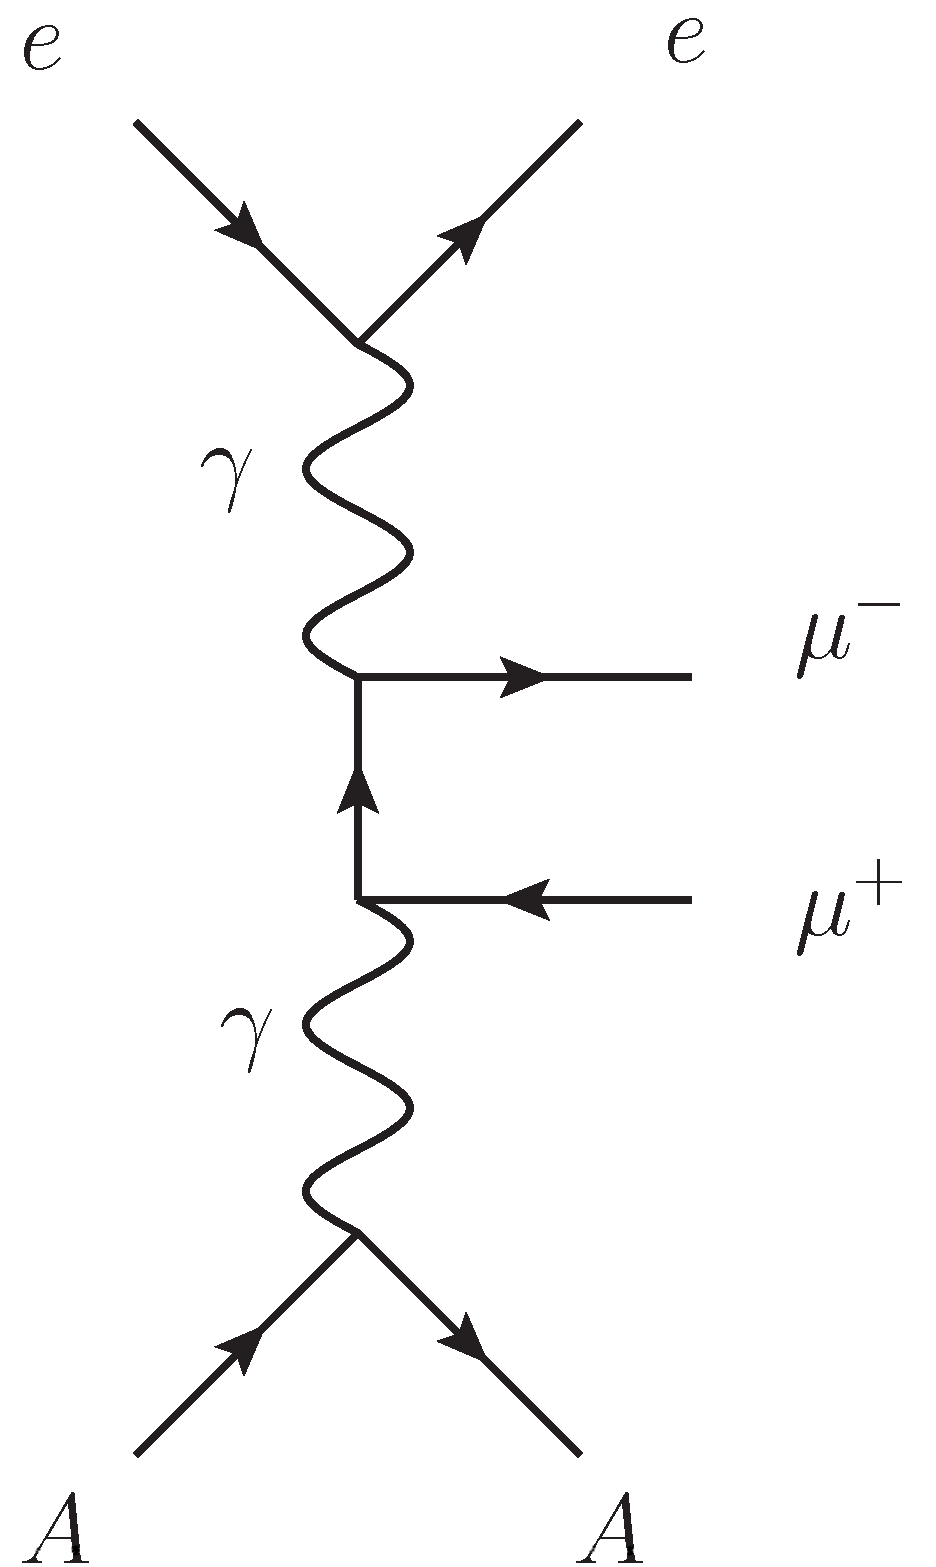
\includegraphics[width=0.5\textwidth]{Feynman_diagrams/Jaxo_BetheHeitler.png}
    \caption{Bethe-Heitler}
    \end{subfigure}\\
    \begin{subfigure}[b]{0.4\textwidth}\centering
    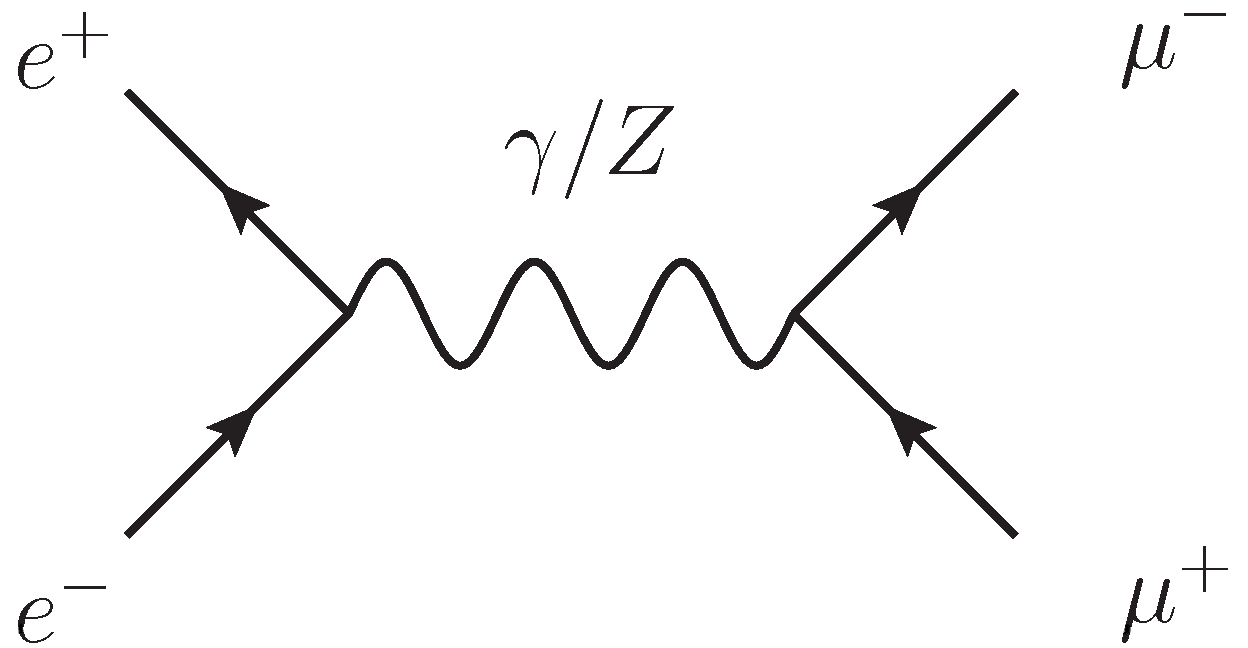
\includegraphics[width=0.7\textwidth]{Feynman_diagrams/Jaxo_annihilation.png}
     \caption{Direct annihilation}
     \end{subfigure}
    \caption[Muon production processes]{
    Feynman diagrams of the muon pair production via the Bethe-Heitler process and the direct annihilation with atomic electrons.}
    \label{fig:BDS_Muons:Muon_production}
\end{wrapfigure}
To prevent the muons from reaching the detectors, two different shielding systems are studied with respect to their effectiveness and feasibility to be integrated in the BDS.
Both systems are based on two ideas: to deflect the muons such that they do not reach the interaction region, and also to stop the muons in the shielding material.
The shielding scenarios that are under discussion foresee a combination of the two systems:
\begin{itemize}
 \item ``5 spoilers'':\\
 In the first scenario, five cylindrical spoilers out of magnetized iron are installed at different locations along the BDS: \SI{1358.5}{\metre}, \SI{1234.5}{\metre}, \SI{1145.5}{\metre}, \SI{975.5}{\metre}, and \SI{802.5}{\metre} from the interaction point (IP), where these locations indicate the midpoint of the spoiler.
 \\The spoilers have a radius of \SI{70}{\centi\meter}, and a length of about \SI{5}{\meter}.
 Their magnetic field ranges from about \SI{19}{\kilo\gauss} in the center of the spoiler to about \SI{10}{\kilo\gauss} at the outer edge~\cite{MuonShielding,Lewis}.
 An illustration of one of these spoilers is given in Figure~\ref{fig:BDS_Muons:shielding_options} (a).
 As indicated by the muon tracks through the spoiler, the magnetic field of the cylindrical spoilers is such that either positively or negatively charged muons are deflected away from the beam path into the tunnel walls.
 \item ``5 spoiler + wall'':\\
 In the second scenario, the same five spoilers are located at the same positions as before.
 But an additional magnetized shielding wall is placed about \SI{400}{\meter} from the interaction point.
 \\The wall is about \SI{5}{\meter} wide and long, and fills out the complete tunnel height.
 Its magnetic field strength is about \SI{16}{\kilo\gauss}~\cite{MuonShielding,Lewis}.
 Figure~\ref{fig:BDS_Muons:shielding_options} (b) shows an illustration of the wall inside the BDS tunnel.
\end{itemize}
The motivation for the study presented in this section is to investigate the effect of the muons on the \sid detector.
The overall goal is to give a recommendation, based on the study of the detector performance, on the necessity of the magnetized in order to keep the detector occupancy below the critical limit of \num{e-4} (as discussed in previous chapters).
Arguments against the wall were brought forward regarding costs and safety issues due to its size in the BDS tunnel.
 \begin{figure}
 \centering
  \begin{subfigure}[b]{0.49\textwidth}
   \centering
    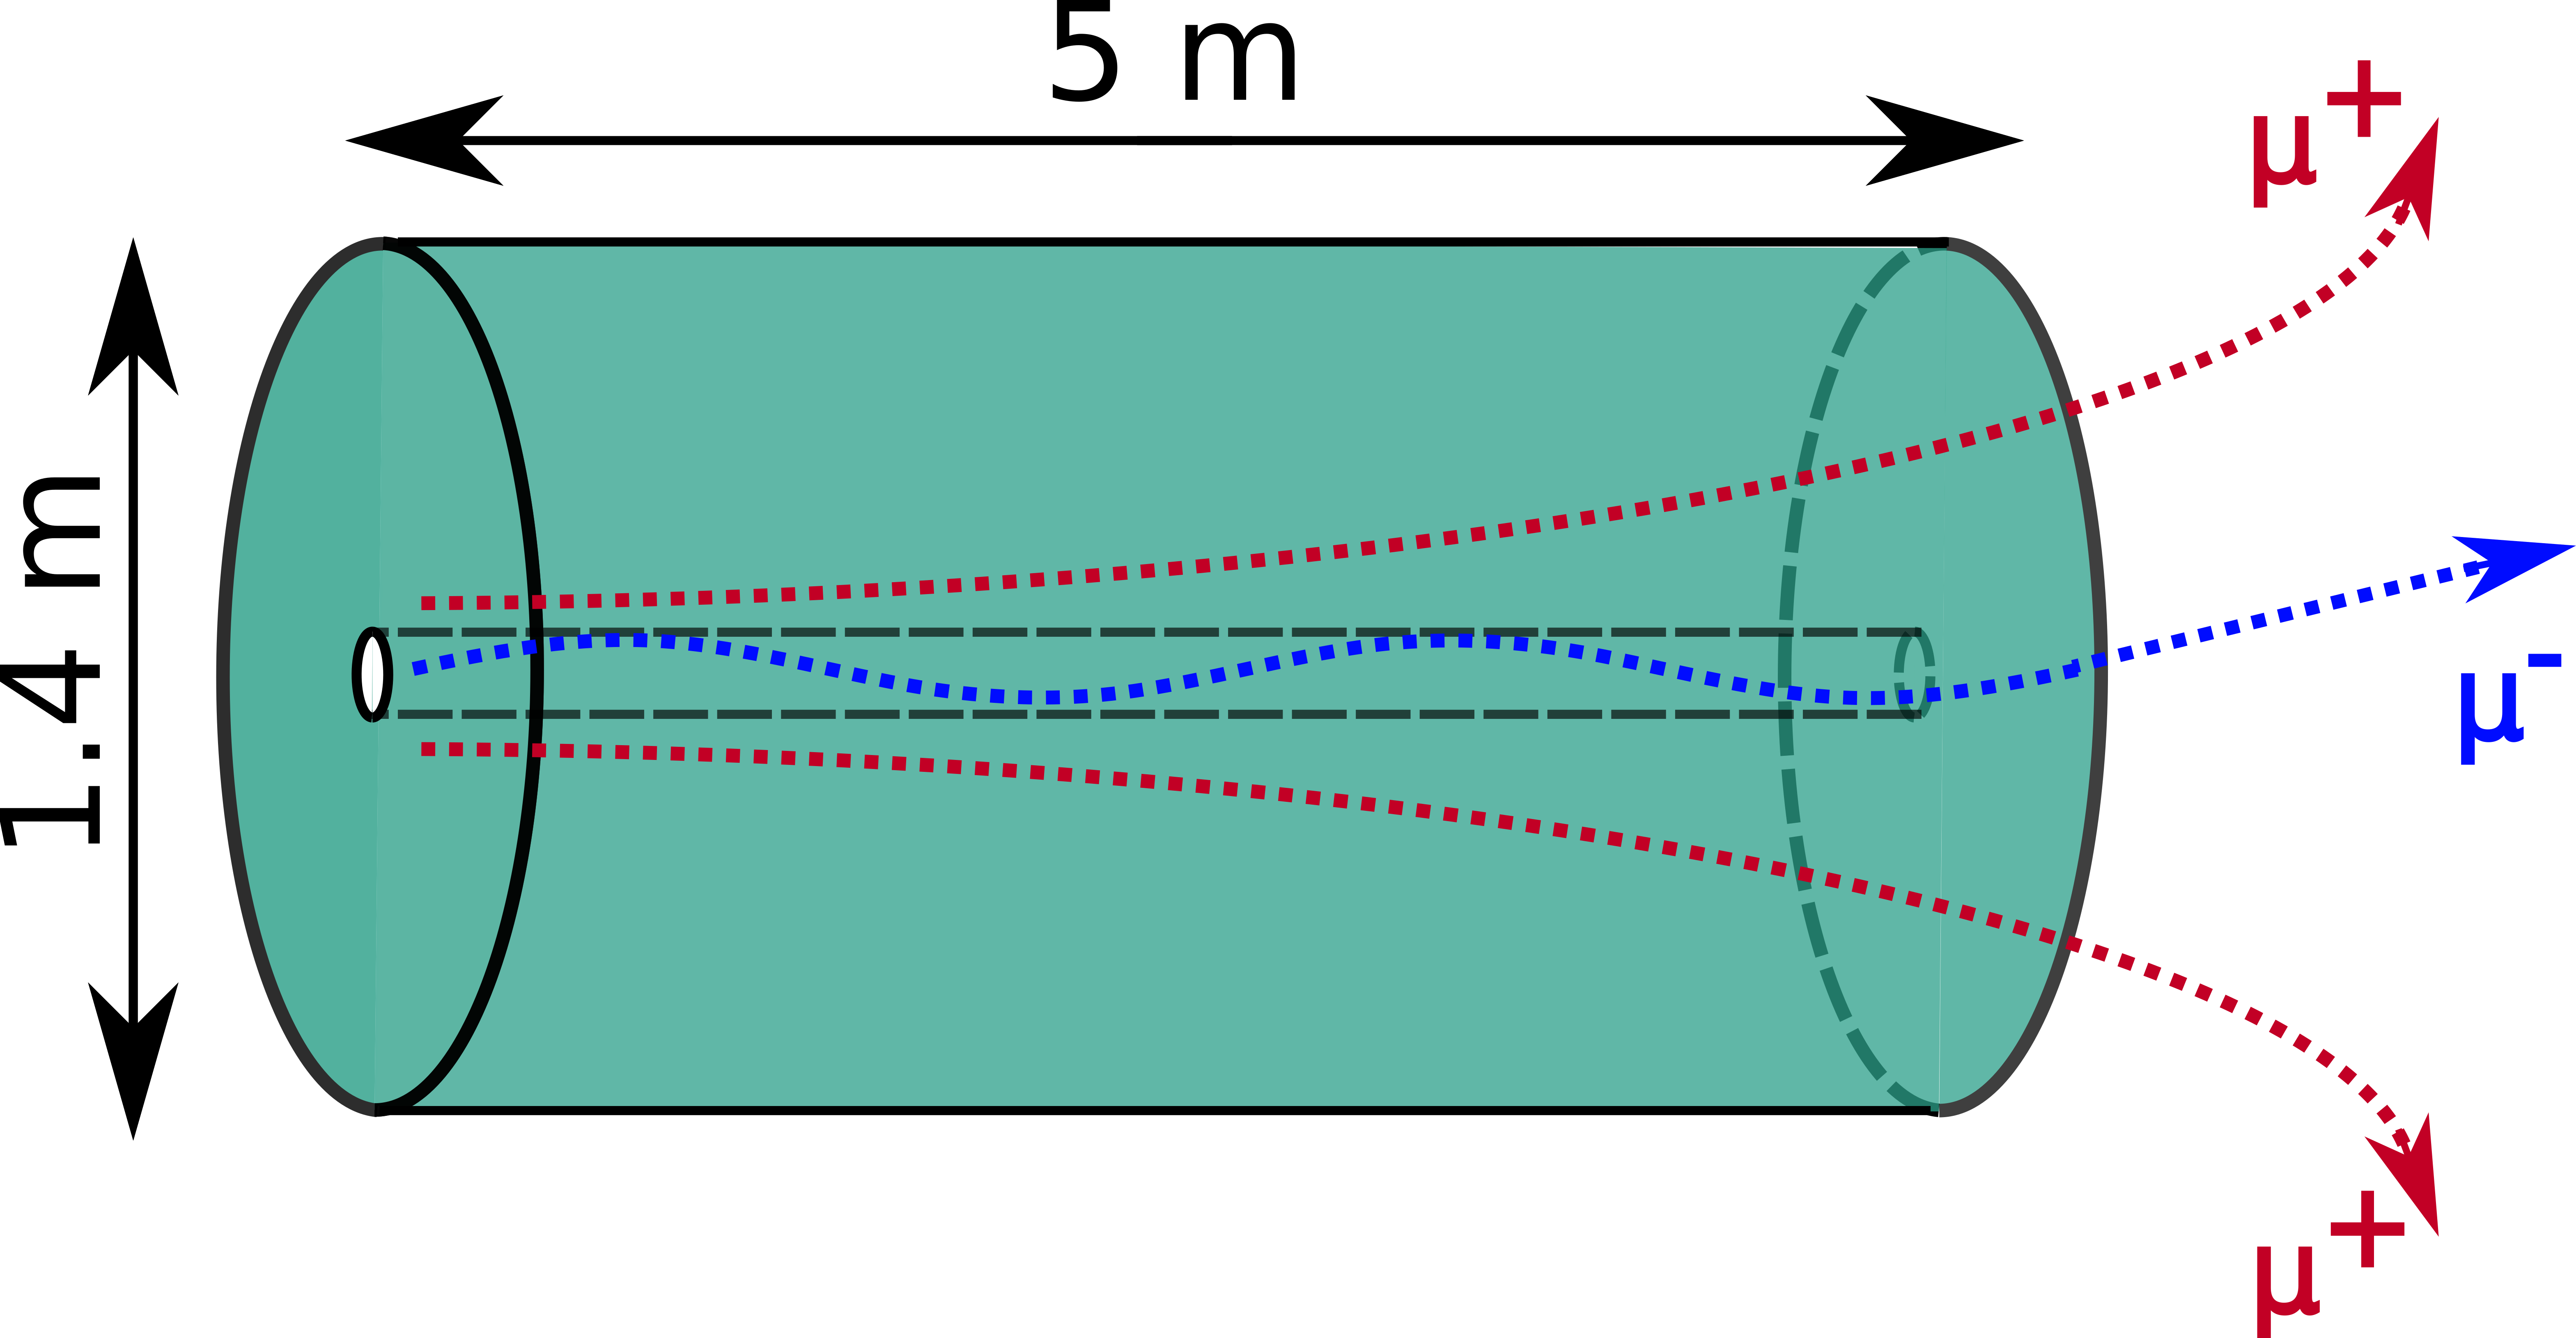
\includegraphics[width=0.7\textwidth]{Figures/BDS_muons/spoilers.png}
   \caption{Cylindrical spoiler}
   \label{fig:spoilers}
   \end{subfigure}
   \hfill
    \begin{subfigure}[b]{0.49\textwidth}
   \centering
    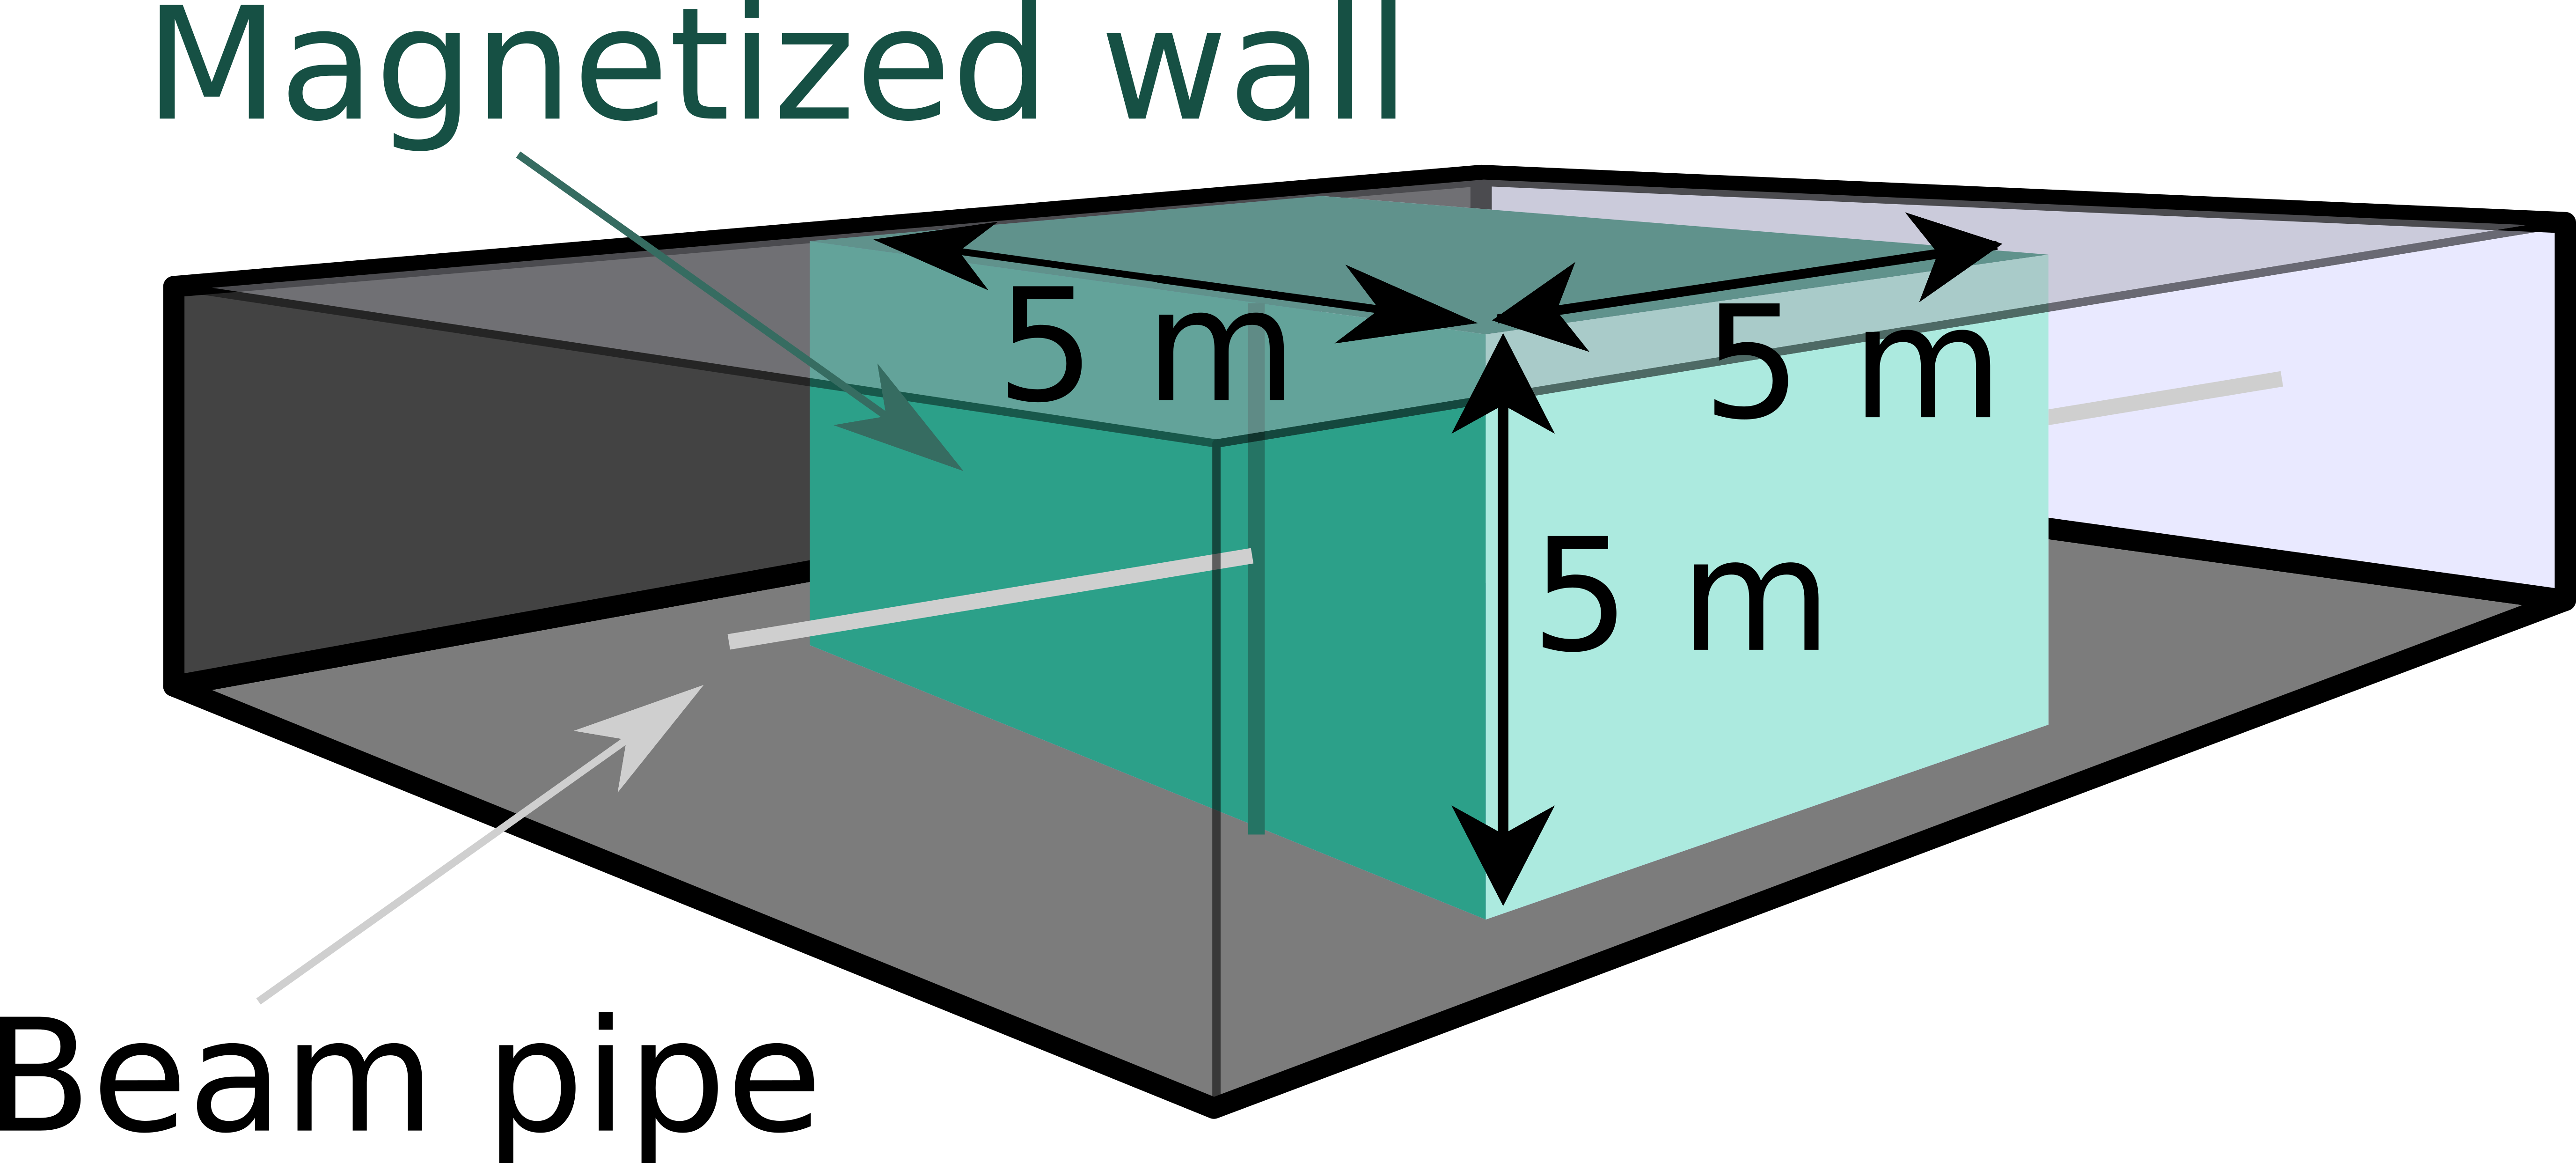
\includegraphics[width=\textwidth]{Figures/BDS_muons/muon_wall.png}
   \caption{Magnetized wall}
   \label{fig:muon_wall}
   \end{subfigure}
   \caption[BDS muon shielding options]{Schematic drawings of the magnetized spoiler (a) and the magnetized shielding wall (b)~\cite[cf. p. 2]{MuonShielding}.
   The magnetized wall is illustrated inside the accelerator tunnel.}
   \label{fig:BDS_Muons:shielding_options}
 \end{figure}

\subsection{\mucarlo}
\label{BDS_Muons:MUCARLO}
The interactions between the ILC beam and the machine components in the BDS were simulated with a Monte Carlo tool called \mucarlo~\cite{Mucarlo,MuonBkg_05TeV,MuonBkg_1TeV}.
Since the presented study is done for two different ILC stages, at \SI{250}{\GeV} and at \SI{500}{\GeV}, the beam parameters of the respective stage were used accordingly.
The geometry lattice of the ILC Beam Delivery System serves as the input geometry to the \mucarlo code, through which the muons are tracked.
Figure~\ref{fig:BDS_Muons:tracks} shows the muon tracks in the electron-line of the BDS.
The muons are created at certain locations along the beam line, are deflected by the magnetic field of beam line components, and lose kinetic energy through scattering in the material of the components the muons hit.
In the end, only those muons that reach the IP (at z = \SI{0}{\meter}) are stored.
Accordingly, Figure~\ref{fig:BDS_Muons:tracks} only shows those muons.
In this plot, there is only one red muon track line, which belongs to a negatively charged muon.
The spoiler polarities are set to defocus muons with the same charge as the beam charge.
Therefore, mainly positively charged muons from the electron beam line will reach the IP.
For the positron beam line, the muons reaching the IP are mainly negatively charged.
\\The main sources of muons were identified in the BDS to be 11 distinct collimators.
The following list names these collimators and their position from the IP~\cite{Lewis}:
\begin{itemize}
 \item Primary collimator spoilers (radiation length: 0.6 X\textsubscript{0}, half-gap\footnote{The term ``half-gap'' is commonly used for collimator systems.
 It describes the gap between one of the collimator jaws and an arbitrarily chosen plane (usually the beam center plane).
 Both of the jaws have the same distance from this plane.}: \SI{930}{\micro\meter} in x, \SI{400}{\micro\meter} in y):\\
  SP2 (\SI{1508}{\meter}), SP4 (\SI{1332}{\meter})
 \item Protection collimators (radiation length: 30 X\textsubscript{0}, inner radius: \SI{0.7}{\centi\meter}):\\
  PC1 (\SI{1452}{\meter}), PC2 (\SI{1387}{\meter}), PC5 (\SI{1276}{\meter}), PC5A (\SI{1242}{\meter}), PC6 (\SI{1208}{\meter}), PC7 (\SI{1047}{\meter})
 \item Absorbers (radiation length: 30 X\textsubscript{0}, half-gap: \SI{0.7}{\centi\meter}):\\
  AB3 (\SI{1420}{\meter}), AB5 (\SI{1237}{\meter}), ABE (\SI{852}{\meter})
\end{itemize}
The protection collimators and absorbers serve the purpose of protecting the magnets of the BDS from particle showers (arising from the beam halo collimation) and from mis-steered primary beams.
The number of muons created is proportional to the fraction of the collimator surface that is hit with respect to the beam size, which was determined with the help of the Monte Carlo ray-tracing computer program \turtle~\cite{Turtle}.
The general design of these collimators can be found in \cite{BDS_coll_design}.
\begin{figure}
\centering
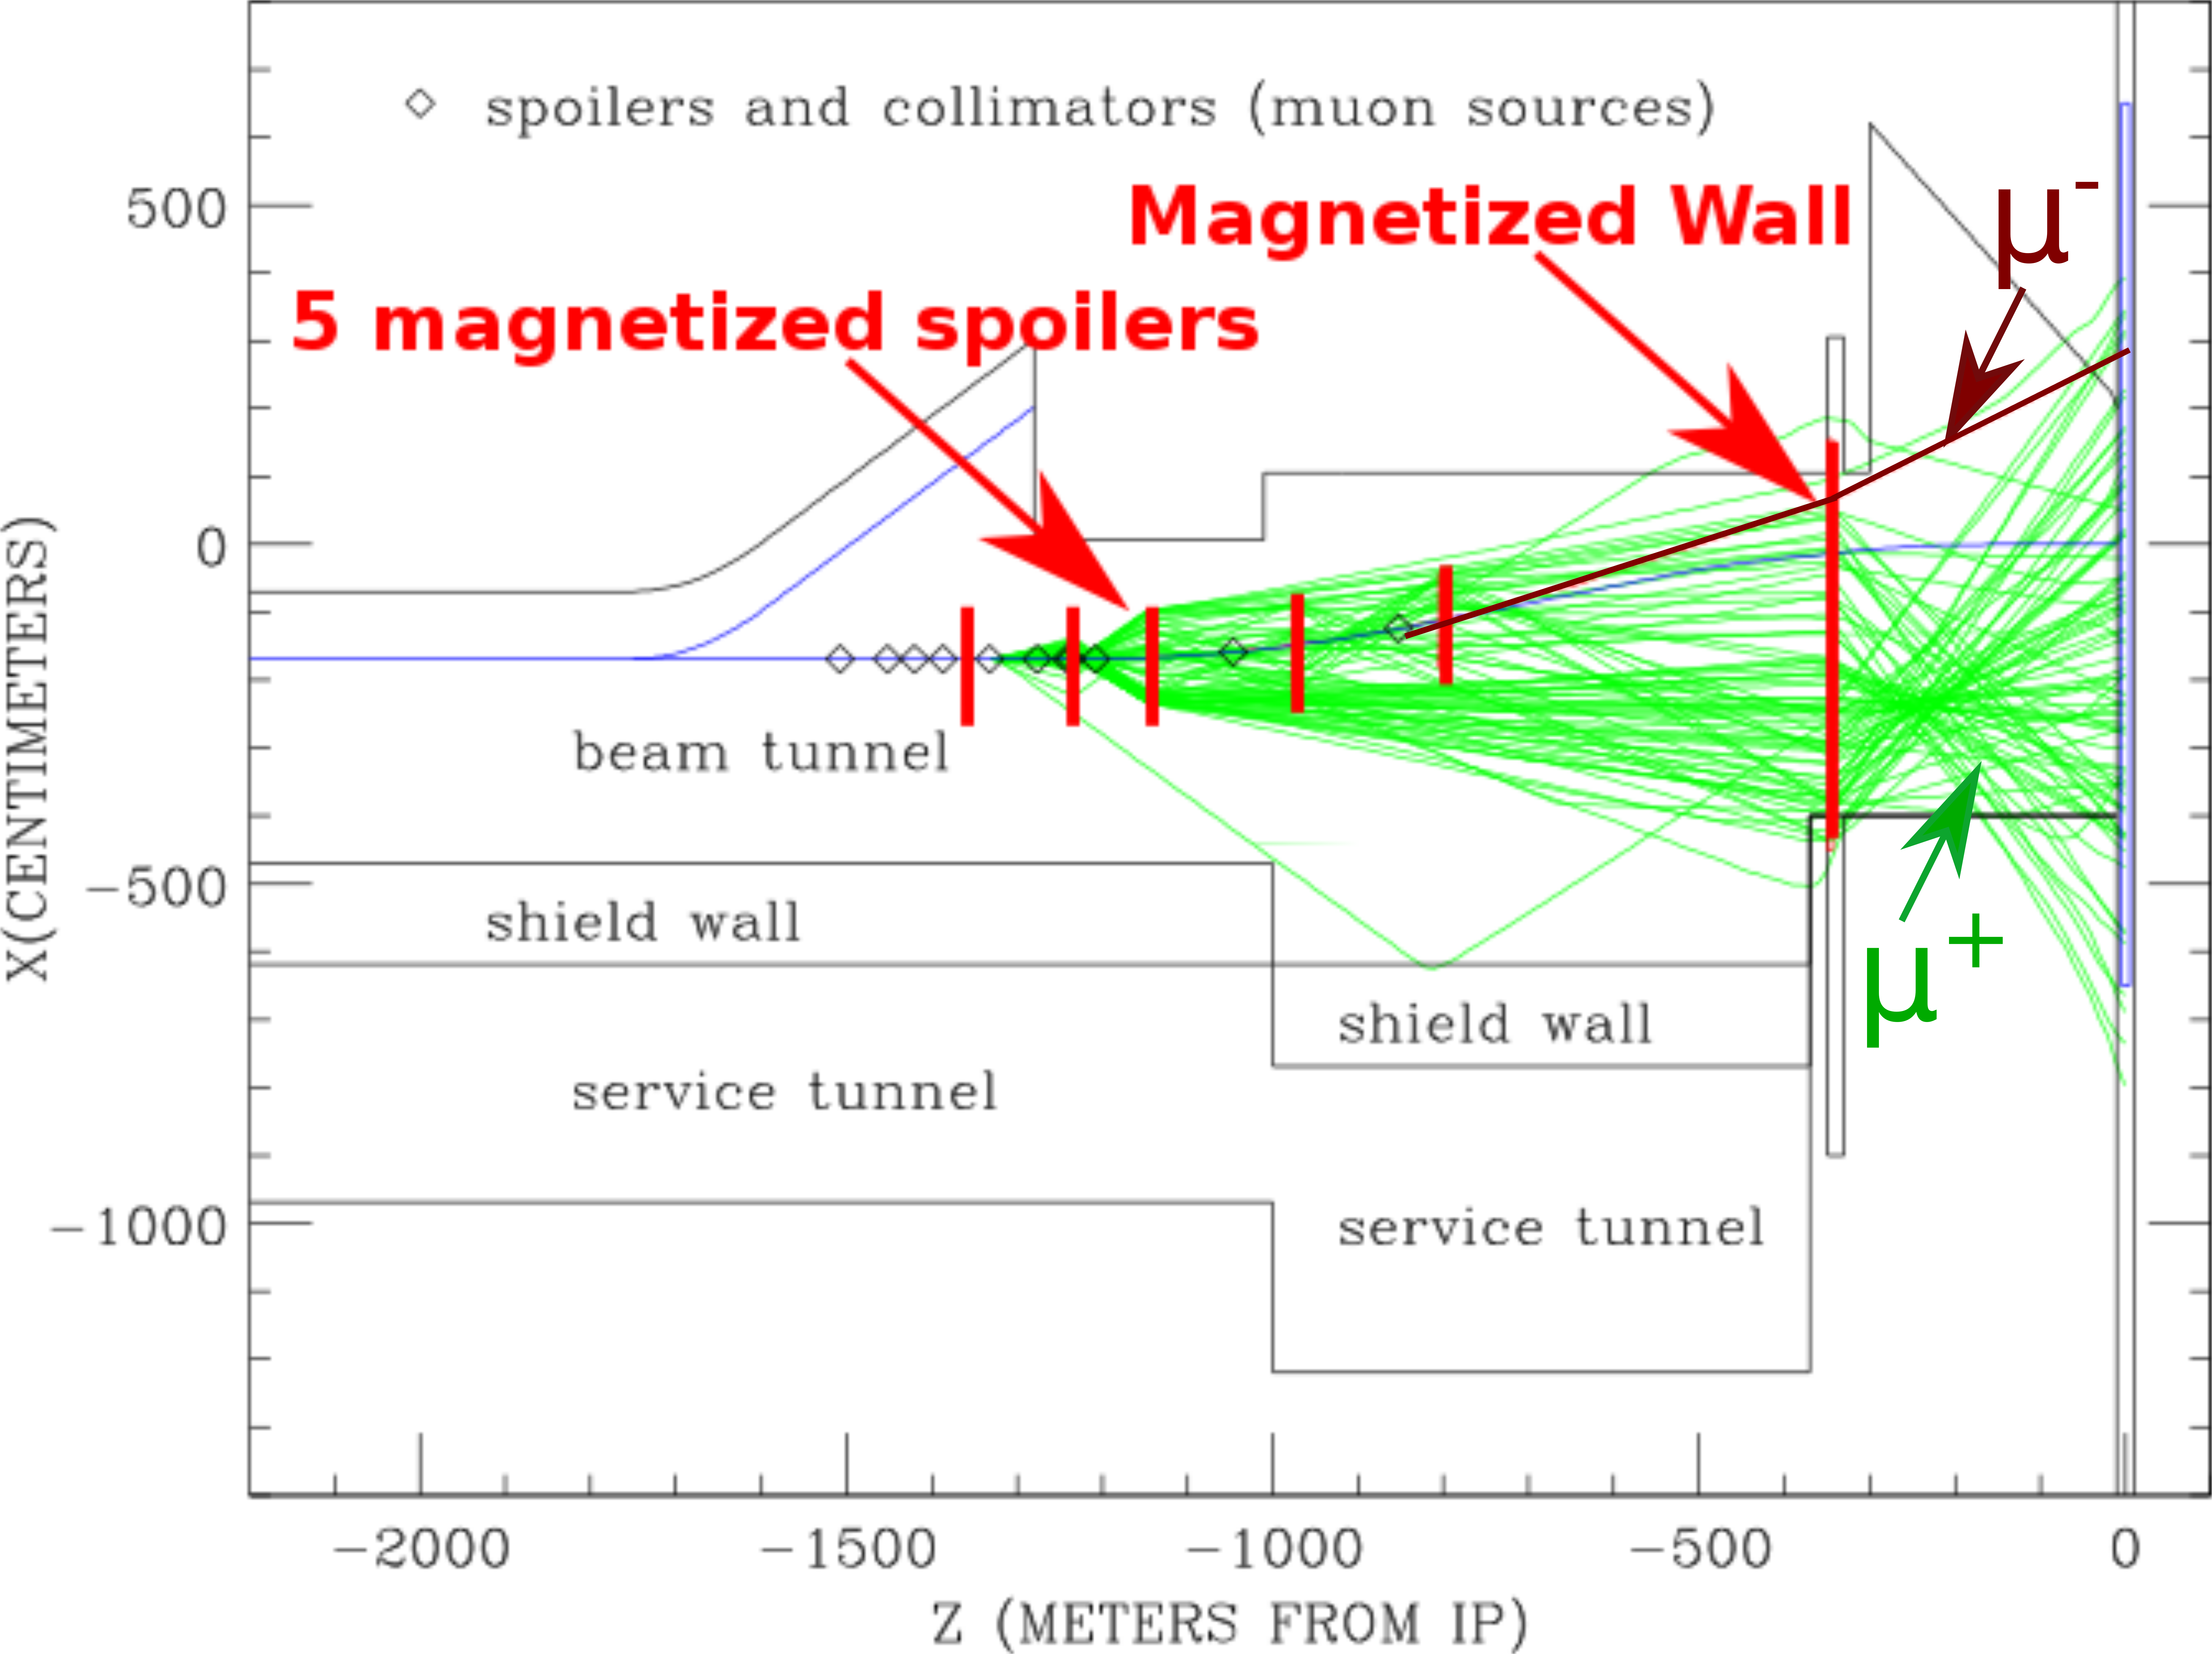
\includegraphics[width=0.6\textwidth]{Figures/BDS_muons/BDS_Tunnel_Spoilers+Wall_edited.png}
\caption[Muon tracks in the Beam Delivery Systems]{Visualization of the muon tracks in the ILC Beam Delivery System (BDS)~\cite{Lewis}.
The picture shows the xz-plane of the BDS tunnel with the beam line components (spoilers and collimators), which serve as muon sources.
In this particular example, the muons origin from the electron beam hitting the primary collimator spoiler SP4.
The locations of the muon shielding components (the magnetized spoilers and wall) are also indicated.
The green/red thin lines represent the tracks of the muons.}
\label{fig:BDS_Muons:tracks}
\end{figure}
Adding up all muons from the different sources on the electron and the positron beam line side, the total number of muons can be calculated that would reach a detector with a radius of \SI{6.5}{\meter} at the interaction region.
Table~\ref{tab:BDS_Muons_muon_numbers} lists the muon rates per bunch crossing for a center-of-mass energy of 250 and \SI{500}{\GeV}, and for the two different shielding scenarios.
At \SI{500}{\GeV}, about 130 muons per bunch crossing would reach the detector in the case that no shielding was installed.
This number is reduced to about 4 muons with the five cylindrical spoilers, and to below 1 muon per bunch crossing with an additional magnetized wall.
For a lower beam energy of \SI{125}{\GeV} (\SI{250}{\GeV} center-of-mass energy), the number of muons that are produced is lower, because of which only around 38 muons reach the detector without shielding.
With the two different shielding scenarios, the muon rate is again reduced significantly to a minimum of about 0.03 per bunch crossing.
%------------------
%\newcolumntype{L}[1]{>{\raggedright\let\newline\\\arraybackslash\hspace{0pt}}m{#1}}
\newcolumntype{C}[1]{>{\centering\let\newline\\\arraybackslash\hspace{0pt}}m{#1}}
%\newcolumntype{R}[1]{>{\raggedleft\let\newline\\\arraybackslash\hspace{0pt}}m{#1}}
%-----------------
\begin{table}[htbp]
\caption[\mucarlo muon rates]{Muon rates per bunch crossing for the two shielding scenarios, gained from \mucarlo simulations~\cite{Lewis}.}
\label{tab:BDS_Muons_muon_numbers}
\centering
\begin{tabularx}{0.56\textwidth}{l|C{3cm}|C{3cm}}
\hline\hline
\textbf{Scenario} & \multicolumn{2}{>{\centering}p{6cm}}{\textbf{Muons per bunch crossing in a detector with 6.5\,m radius}}\\
& ILC500 & ILC250\\
\hline
 No Spoilers & 130 & 38\\
 5 spoilers& 4.3 & 1.3\\
 5 spoilers + wall & 0.6 &  0.03\\
\hline\hline
\end{tabularx}
\end{table}
\\The output of \mucarlo is a text file containing the four-vectors of the muons \SI{10}{\meter} from the IP.
These four-vectors can therefore be used as input to a full detector simulation. 
\\An additional study was done using a \geant simulation of the BDS tunnel in order to cross check the \mucarlo results and to thereby verify the \mucarlo simulation.
The outcome of that study was that both simulations are in good agreement~\cite{Glens_muon_talk}.

\subsection{Effect of muons on the \sid performance}
\label{BDS_Muons:SiD}
Since the \sid detector only reads out the hits after every bunch train (1312 bunch crossings), the detector occupancy for the muons has to be studied for a muon rate per train.
As in the previous chapter, the full detector simulation was done using \slic.
The geometry input file that was used contained the most recent sidloi3 geometry of the \sid detector, including the new L* position, the anti-DiD field, as well as the Pacman geometry.
For details on these detector characteristics, please refer to Section~\ref{ILC:SiD}.
After a file-format conversion, the \mucarlo output files containing the four-vectors of the muons for the different shielding scenarios and center-of-mass energies served as the particle source input to \slic.

\subsubsection{Muon hit distribution}
For visualizing the hit distribution in the \sid detector, event displays (see Figure~\ref{fig:BDS_Muons:wired4}) were made using WIRED4~\cite{Wired4}.
 \begin{figure}[htbp]
 \centering
  \begin{subfigure}[b]{0.31\textwidth}
   \centering
   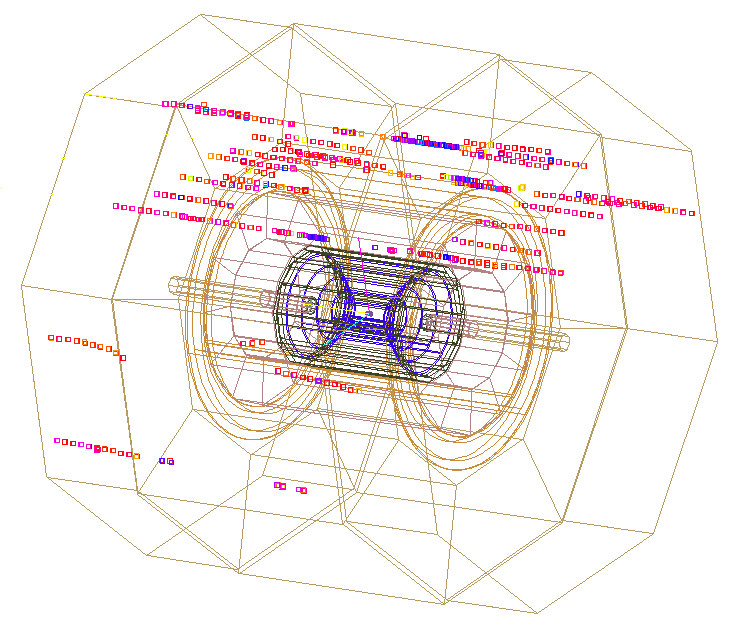
\includegraphics[width=\textwidth]{Figures/BDS_muons/Event_display_ILC250_p_spoilers_wall_inverted.png}
   \caption{3D view, 5 spoilers + wall,\\ILC250}
   \end{subfigure}
   \hfill
   \begin{subfigure}[b]{0.31\textwidth}
   \centering
    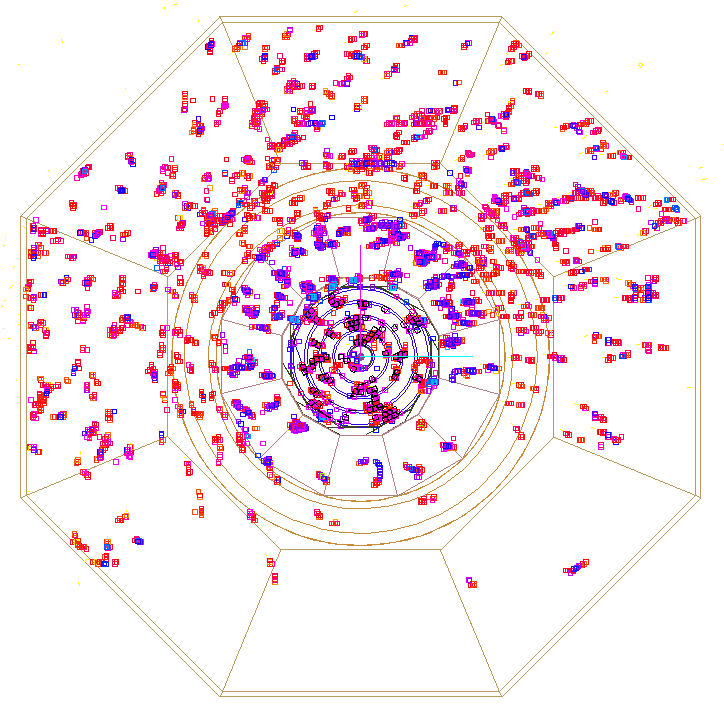
\includegraphics[width=0.9\textwidth]{Figures/BDS_muons/muons_positron_5spoilers_wall_515_xyview_croped_inverted.png}
   \caption{xy-view, 5 spoilers + wall,\\ILC500}
   \end{subfigure}
   \hfill
    \begin{subfigure}[b]{0.31\textwidth}
   \centering
    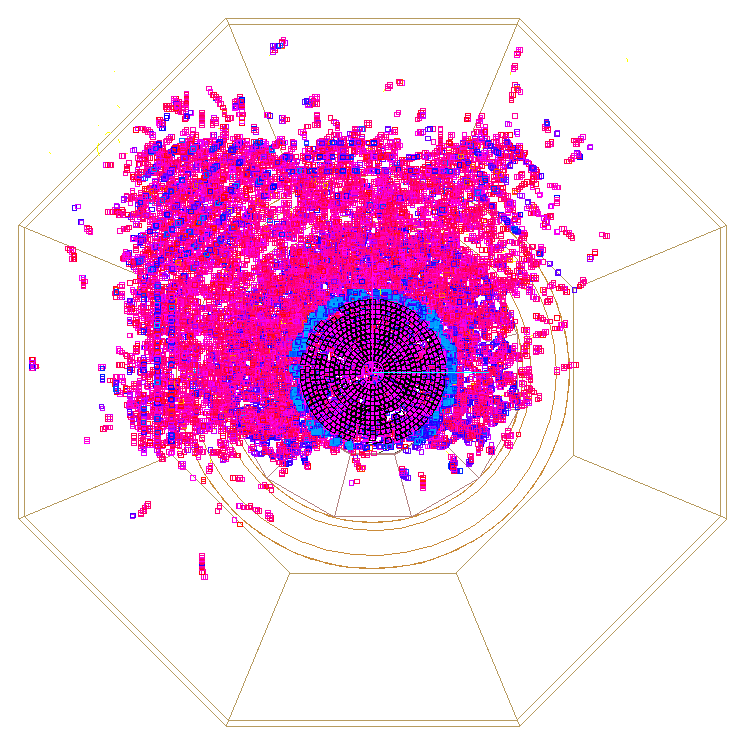
\includegraphics[width=0.9\textwidth]{Figures/BDS_muons/muons_positron_5spoilers_2961_xyview_croped_inverted.png}
   \caption{xy-view, 5 spoilers,\\ILC500}
   \end{subfigure}
   \caption[Event displays of BDS muons in \sid]{Event displays of the muon hits in \sid for different center-of-mass energies and different shielding scenarios.}
   \label{fig:BDS_Muons:wired4}
 \end{figure}
\\Apart from the overall number of hits in the different event displays, the spatial distribution of the hits is striking.
Concentrating on Figure~\ref{fig:BDS_Muons:wired4} (a) first, the muons leave clear horizontal tracks throughout the whole detector.
After leaving the BDS tunnel, the muons (which are boosted in forward direction) enter \sid through the outermost subdetector, and penetrate the full detector.
Since the muons are coming from both the electron and the positron beam line, this happens simultaneously from both sides.
\\The difference in the spatial distribution in the xy-plane between Figure~\ref{fig:BDS_Muons:wired4} (b) and (c) is explained by the geometry of the tunnel, and position of the detector with respect to the tunnel exit.
In subfigure (a), the rectangular shape in the hit distribution is the imprint of the tunnel.
The boosted muons exit the tunnel and directly hit the detector.
The asymmetry of the imprint results from the position of the detector.
The beam pipe and therefore the central axis through the detectors are not in the center of the BDS tunnel.
As can be seen in Figure~\ref{fig:BDS_Muons:tracks}, the beam line curves such that it is closer to one of the tunnel side walls than to the other.
The top-bottom asymmetry is due to the fact that the detector cavern is below ground level of the tunnel.
\\Adding the magnetized wall as an additional muon shielding causes the muons to scatter.
The clear tunnel imprint is no longer visible in Figure~\ref{fig:BDS_Muons:wired4} (b).
Scattering the muons is not the only effect of the magnetized wall.
As can be seen in Figure~\ref{fig:BDS_Muons:energy}, the wall shifts the muon energy to lower values for a respective center-of-mass energy.
The muons are deflected away from the forward directions due to the magnetization of the wall, but also lose their energy in the material of the wall.
Low energy muons are either stopped completely, or deflected such that they cannot reach the detector. %\todo{Check out Bethe-Bloch here}
The peak in the energy distributions at lower energies is therefore reduced for the ``5 spoilers + wall'' scenarios.
Additionally, the number of muons per bunch train can directly be compared for the two ILC stages and the different shielding options.
\begin{figure}[htbp]
\centering
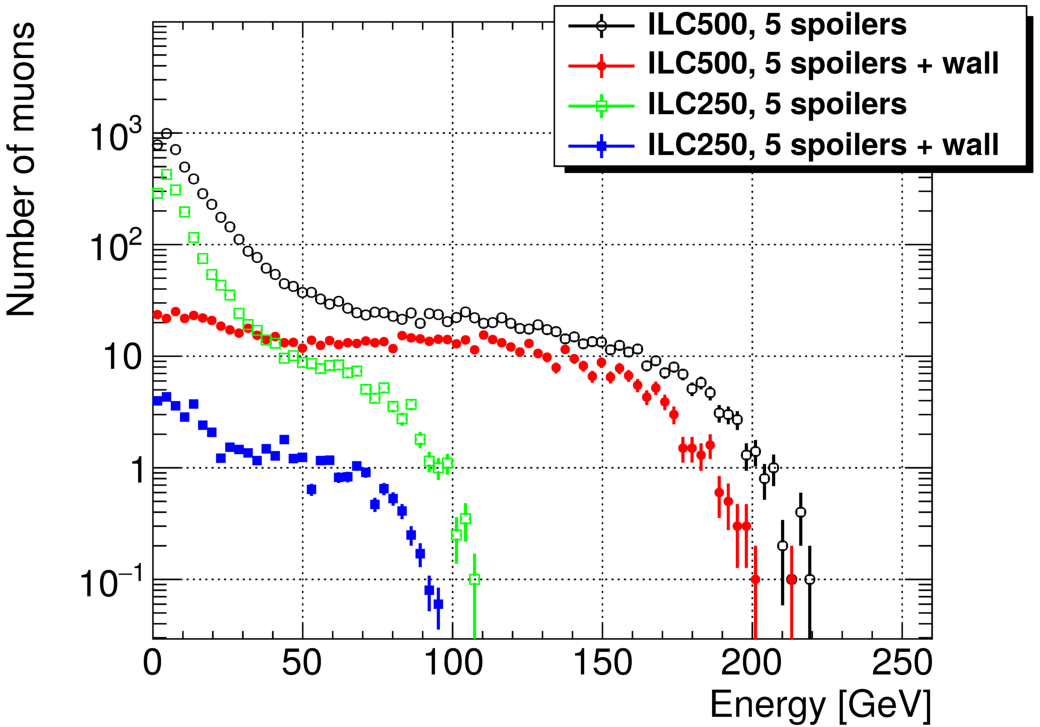
\includegraphics[width=0.6\textwidth]{Figures/BDS_muons/Energy_Comparison_ILC500vsILC250.pdf}
\caption[Muon energy]{Energy distribution of the muons for the different shielding scenarios, and for a center-of-mass energy of 250 and \SI{500}{\GeV}.
The number of muons are normalized to a full bunch train for all cases.}
\label{fig:BDS_Muons:energy}
\end{figure}
\\These muons then leave a particular number of hits in the \sid subdetectors by penetrating the full detector.
For the comparison between the total number of hits in the four different cases, Figure~\ref{fig:BDS_Muons:hits} shows a bar chart of the hits collected in each subdetector.
The largest number of hits is counted for the endcaps of the muon detector system, which is the subdetector with the largest effective detector area under normal incident of the muons.
Also, it is the outermost subdetector, likely to be hit by all of the primary muons.
Accordingly, the vertex detector (as the smallest and innermost detector) is hit the least number of times, and in the same manner also the other subdetectors gain representative number of hits.
Deducing from the hit distributions, the \sid detector will overall suffer from less hits in the ILC250 stage with respect to the ILC500, but adding the magnetized wall to the shielding will yield even smaller hit counts for both center-of-mass energies.
\begin{figure}[h]
\centering
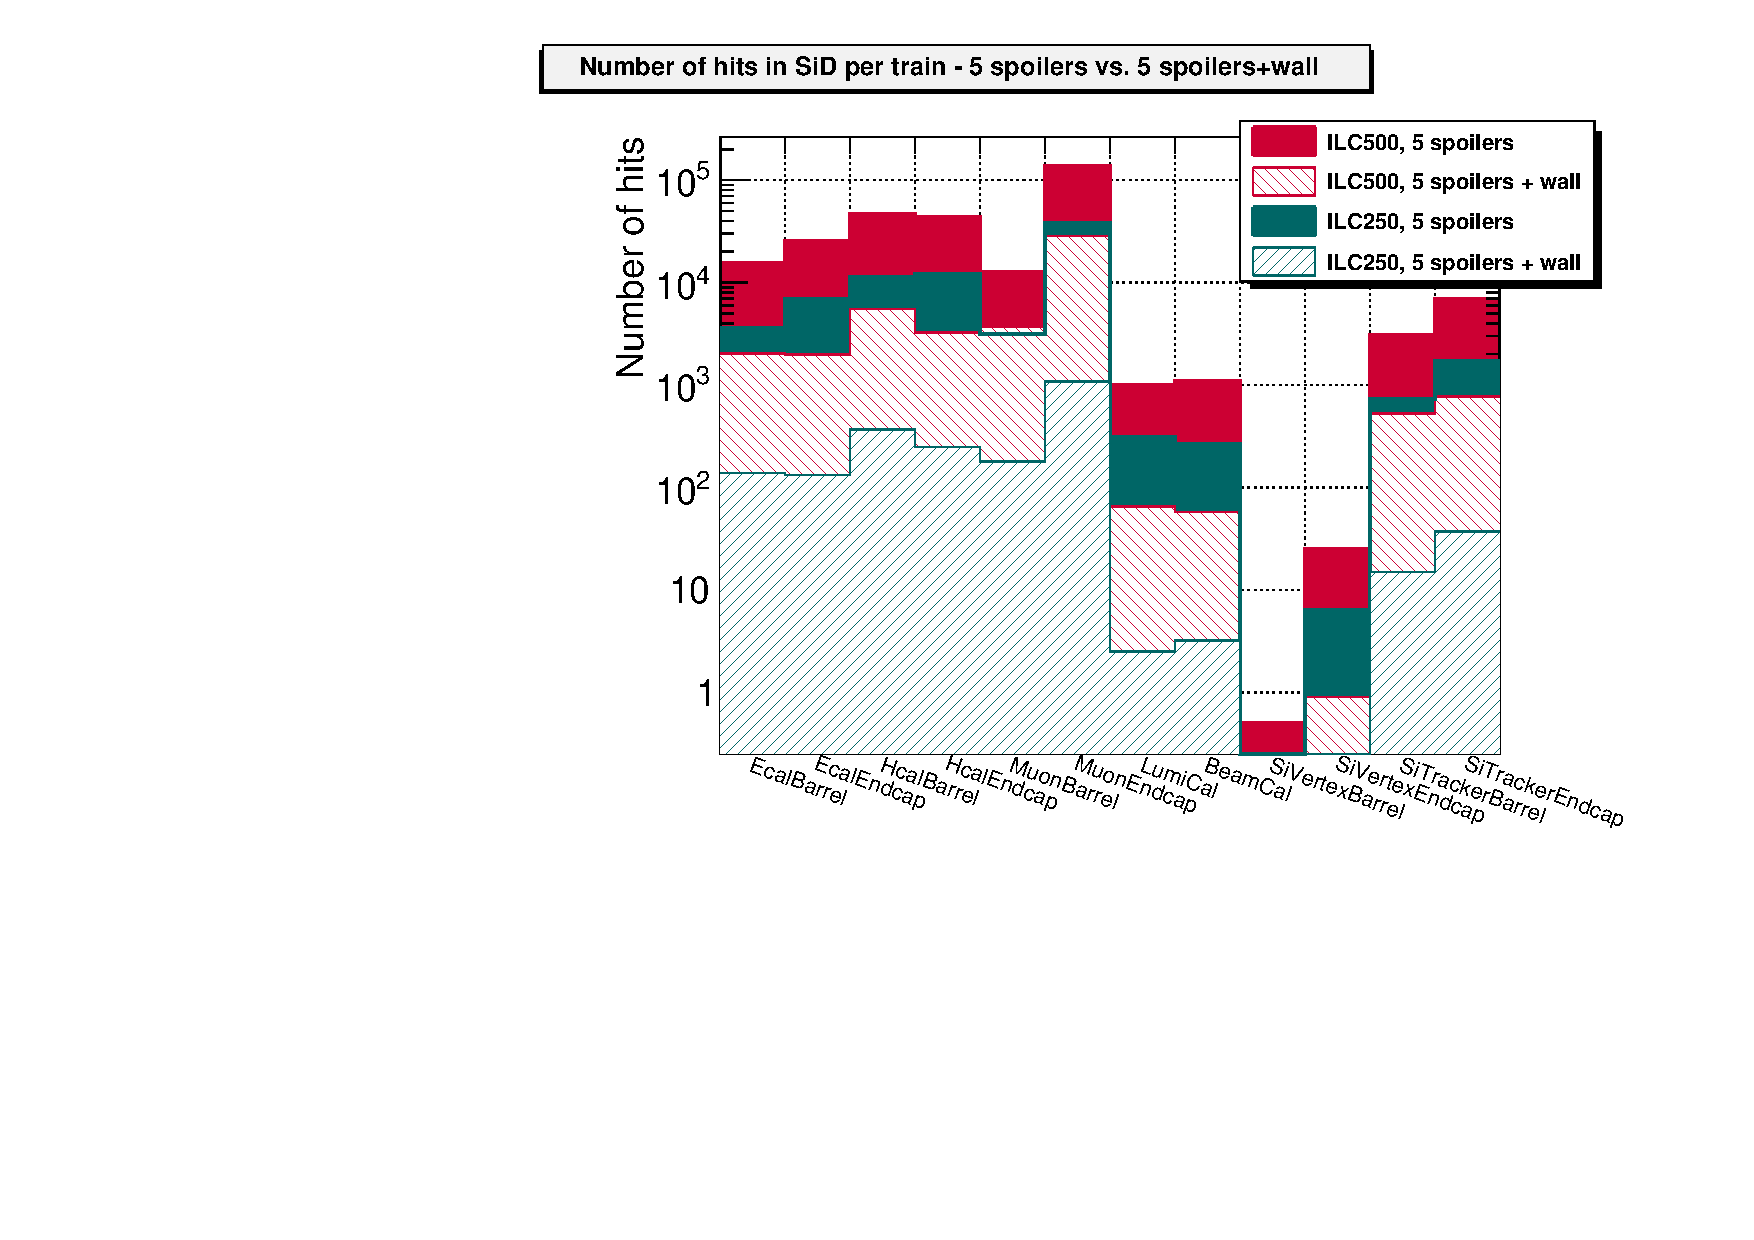
\includegraphics[width=0.7\textwidth]{Figures/BDS_muons/Hits_in_SiD_subdetectors_MuonSpoilerStudy.pdf}
\caption[Number of muon hits in the \sid subdetectors]{Total number of hits in the various \sid subdetectors for both shielding scenarios and both ILC stages.
The number of hits come from muons from a full bunch train.}
\label{fig:BDS_Muons:hits}
\end{figure}
\\After looking at the total number of hits, which reflects the size and position of the subdetectors in \sid, this fact can be even better derived from the hit time distributions shown in Figure~\ref{fig:BDS_Muons:hittime}.
The muons emitted from the BDS tunnel arrive first at the endcaps of the muon system, as mentioned above.
After penetrating all muon endcap layers, the next outermost subdetector is hit and so on, until the muons make their way to the opposite muon endcap.
The time needed for the muons to penetrate the full detector is hence about \SI{40}{\nano\second}, independent of the muon shielding and the center-of-mass energy.
\begin{figure}[htbp!]
\centering
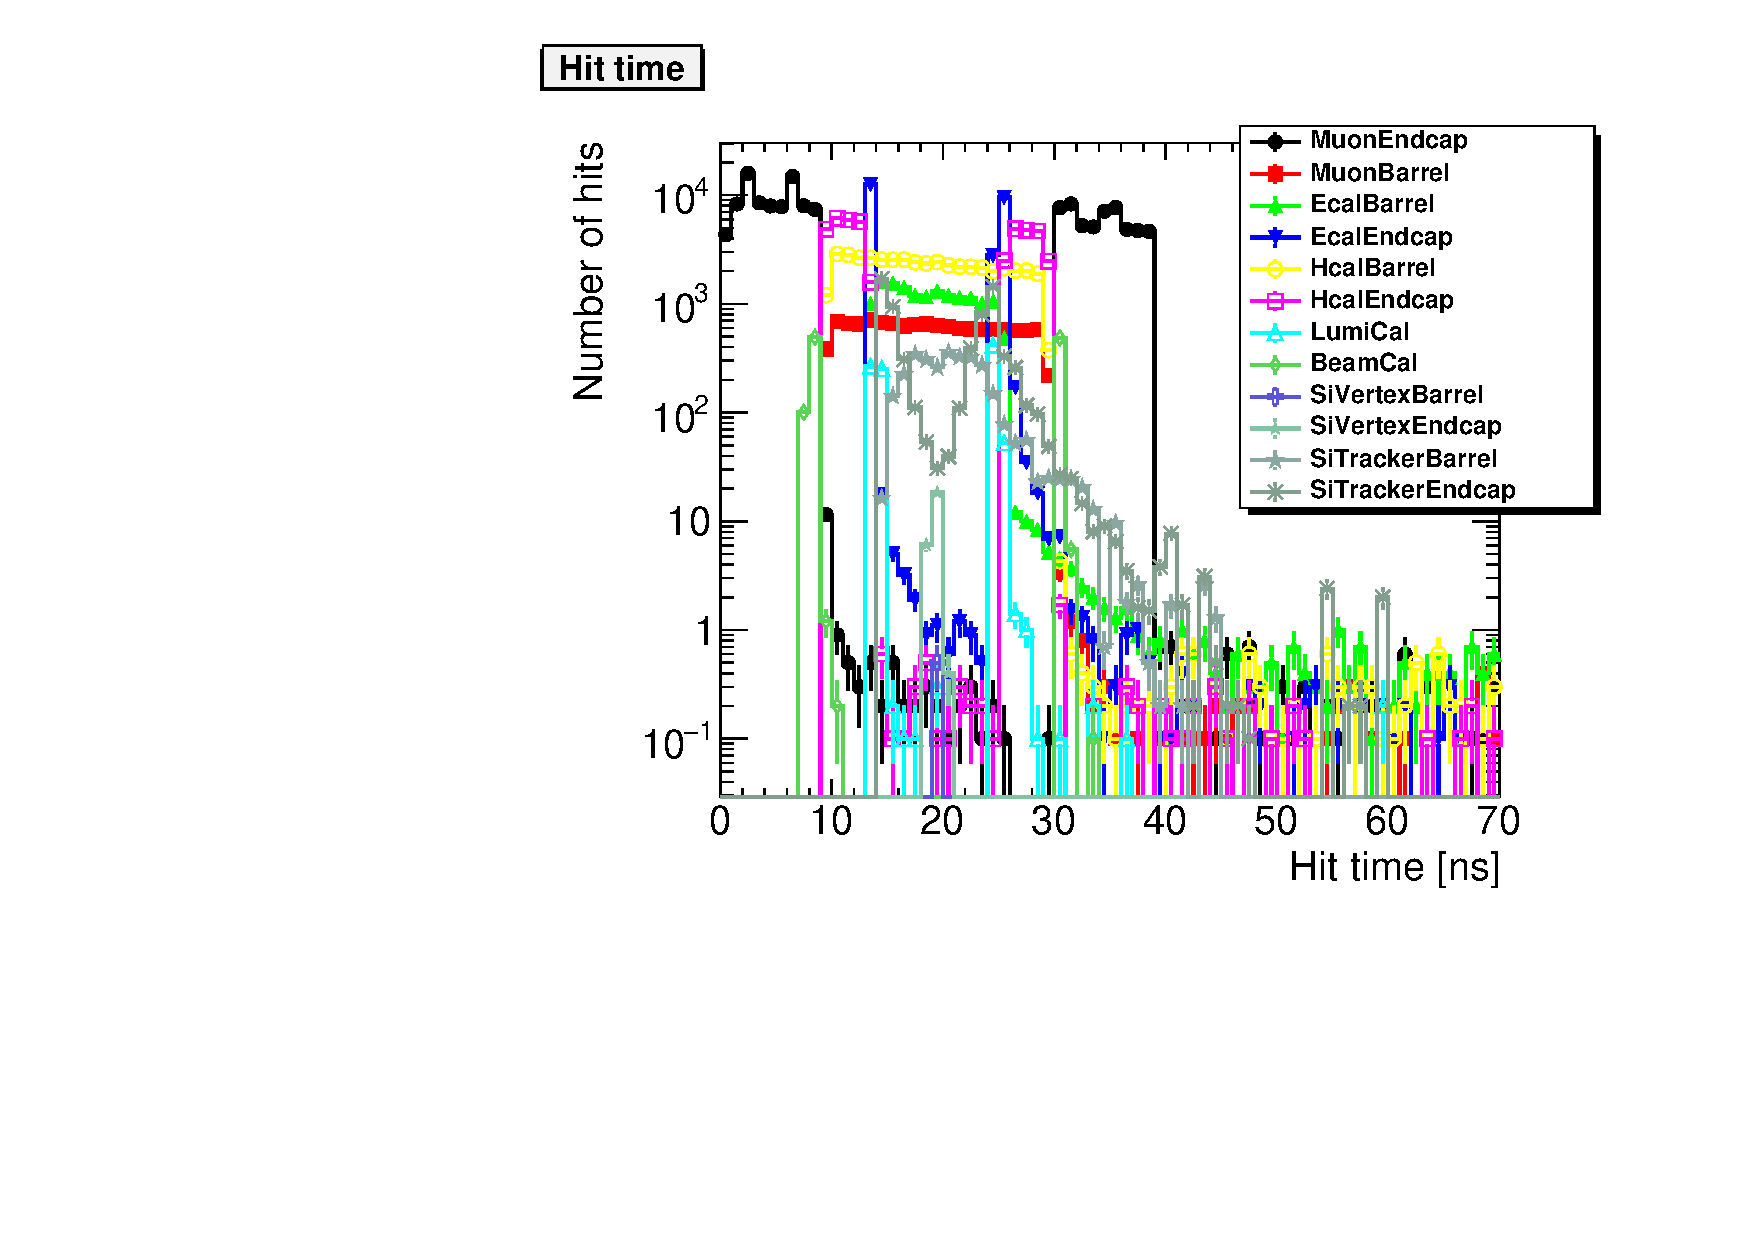
\includegraphics[width=0.7\textwidth]{Figures/BDS_muons/hittime_ILC500_spoilers_superimposed.pdf}
\caption[Muon hit time in the \sid subdetectors]{Hit time distribution of the BDS muons in the various \sid subdetectors for ILC500 stage and for the ``5 spoilers'' scenario only.
The number of hits are normalized to hits from a full bunch train for all cases.}
\label{fig:BDS_Muons:hittime}
\end{figure}

\subsubsection{\sid occupancy}
\label{BDS_Muons:sidocc}
The next step is to look at the occupancy of the detector arising from these muon hits.
As in Chapter~\ref{PairBkg:occupancy}, the number of hits are counted for every cell in the subdetectors, which can be directly translated into a detector occupancy.
In the following, the muon occupancy in the \sid HCAL barrel and the tracker endcaps is discussed.
As explained in the previous chapter, occupancy plots show how many detector cells are hit a certain number of times. 
By respecting the rule that the sum of all cells with a number of hits greater than or equal to the buffer depth should not exceed \SI{0.01}{\percent} (\num{e-4} of all cells), a statement can be made whether given occupancy levels are acceptable.
By optimizing the design of the detectors and the accelerator, a balance can be found between a sufficient buffer depth of the detector sensors and low background levels arising from the accelerator.
\\Figure~\ref{fig:BDS_Muons:HcalBarrel} shows the occupancy and the number of dead cells~\footnote{A cell is defined to be dead when the buffer of its sensor is already completely filled, and no further hits can be stored. Further details can be found in Chapter~\ref{PairBkg:occupancy}.} in the HCAL barrel, normalized to its total number of cells.
In the current detector design, the HCAL cells have a size of \SI{1}{\centi\meter}$\times$\SI{1}{\centi\meter}.
As a result, a maximum of three hits per cell is observed, because of which the x-axis range in Figure~\ref{fig:BDS_Muons:HcalBarrel} (b) also reaches to three only.
Here, the number of dead cells is shown as a function of the assumed buffer depth.
In the theoretical case of a buffer depth of one, about \num{e-4} of all cells would have a full buffer (with one hit) for the ``5 spoilers'' case in the ILC500.
Here, the critical limit for acceptable occupancies of \num{e-4} would just about be reached, all other cases would have acceptable values.
Realistically, the HCAL sensor will have a higher buffer depth, namely a buffer depth of four (in the current design) or higher.
Since none of the cells are hit by more than three muons, the occupancy in the HCAL barrel is very low and far from the critical limit.
 \begin{figure}
 \centering
  \begin{subfigure}[b]{0.49\textwidth}
   \centering
    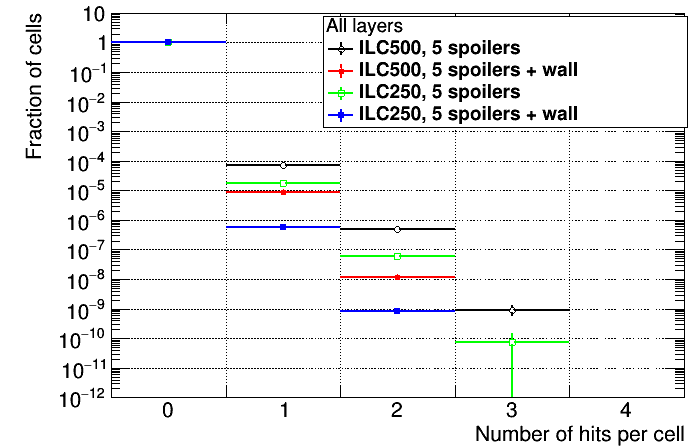
\includegraphics[width=\textwidth]{Figures/BDS_muons/Occupancy_Comparison_All_layers_wrt_cells_HcalBarrel.png}
   \caption{Normalized occupancy}
   \end{subfigure}
   \hfill
    \begin{subfigure}[b]{0.49\textwidth}
   \centering
    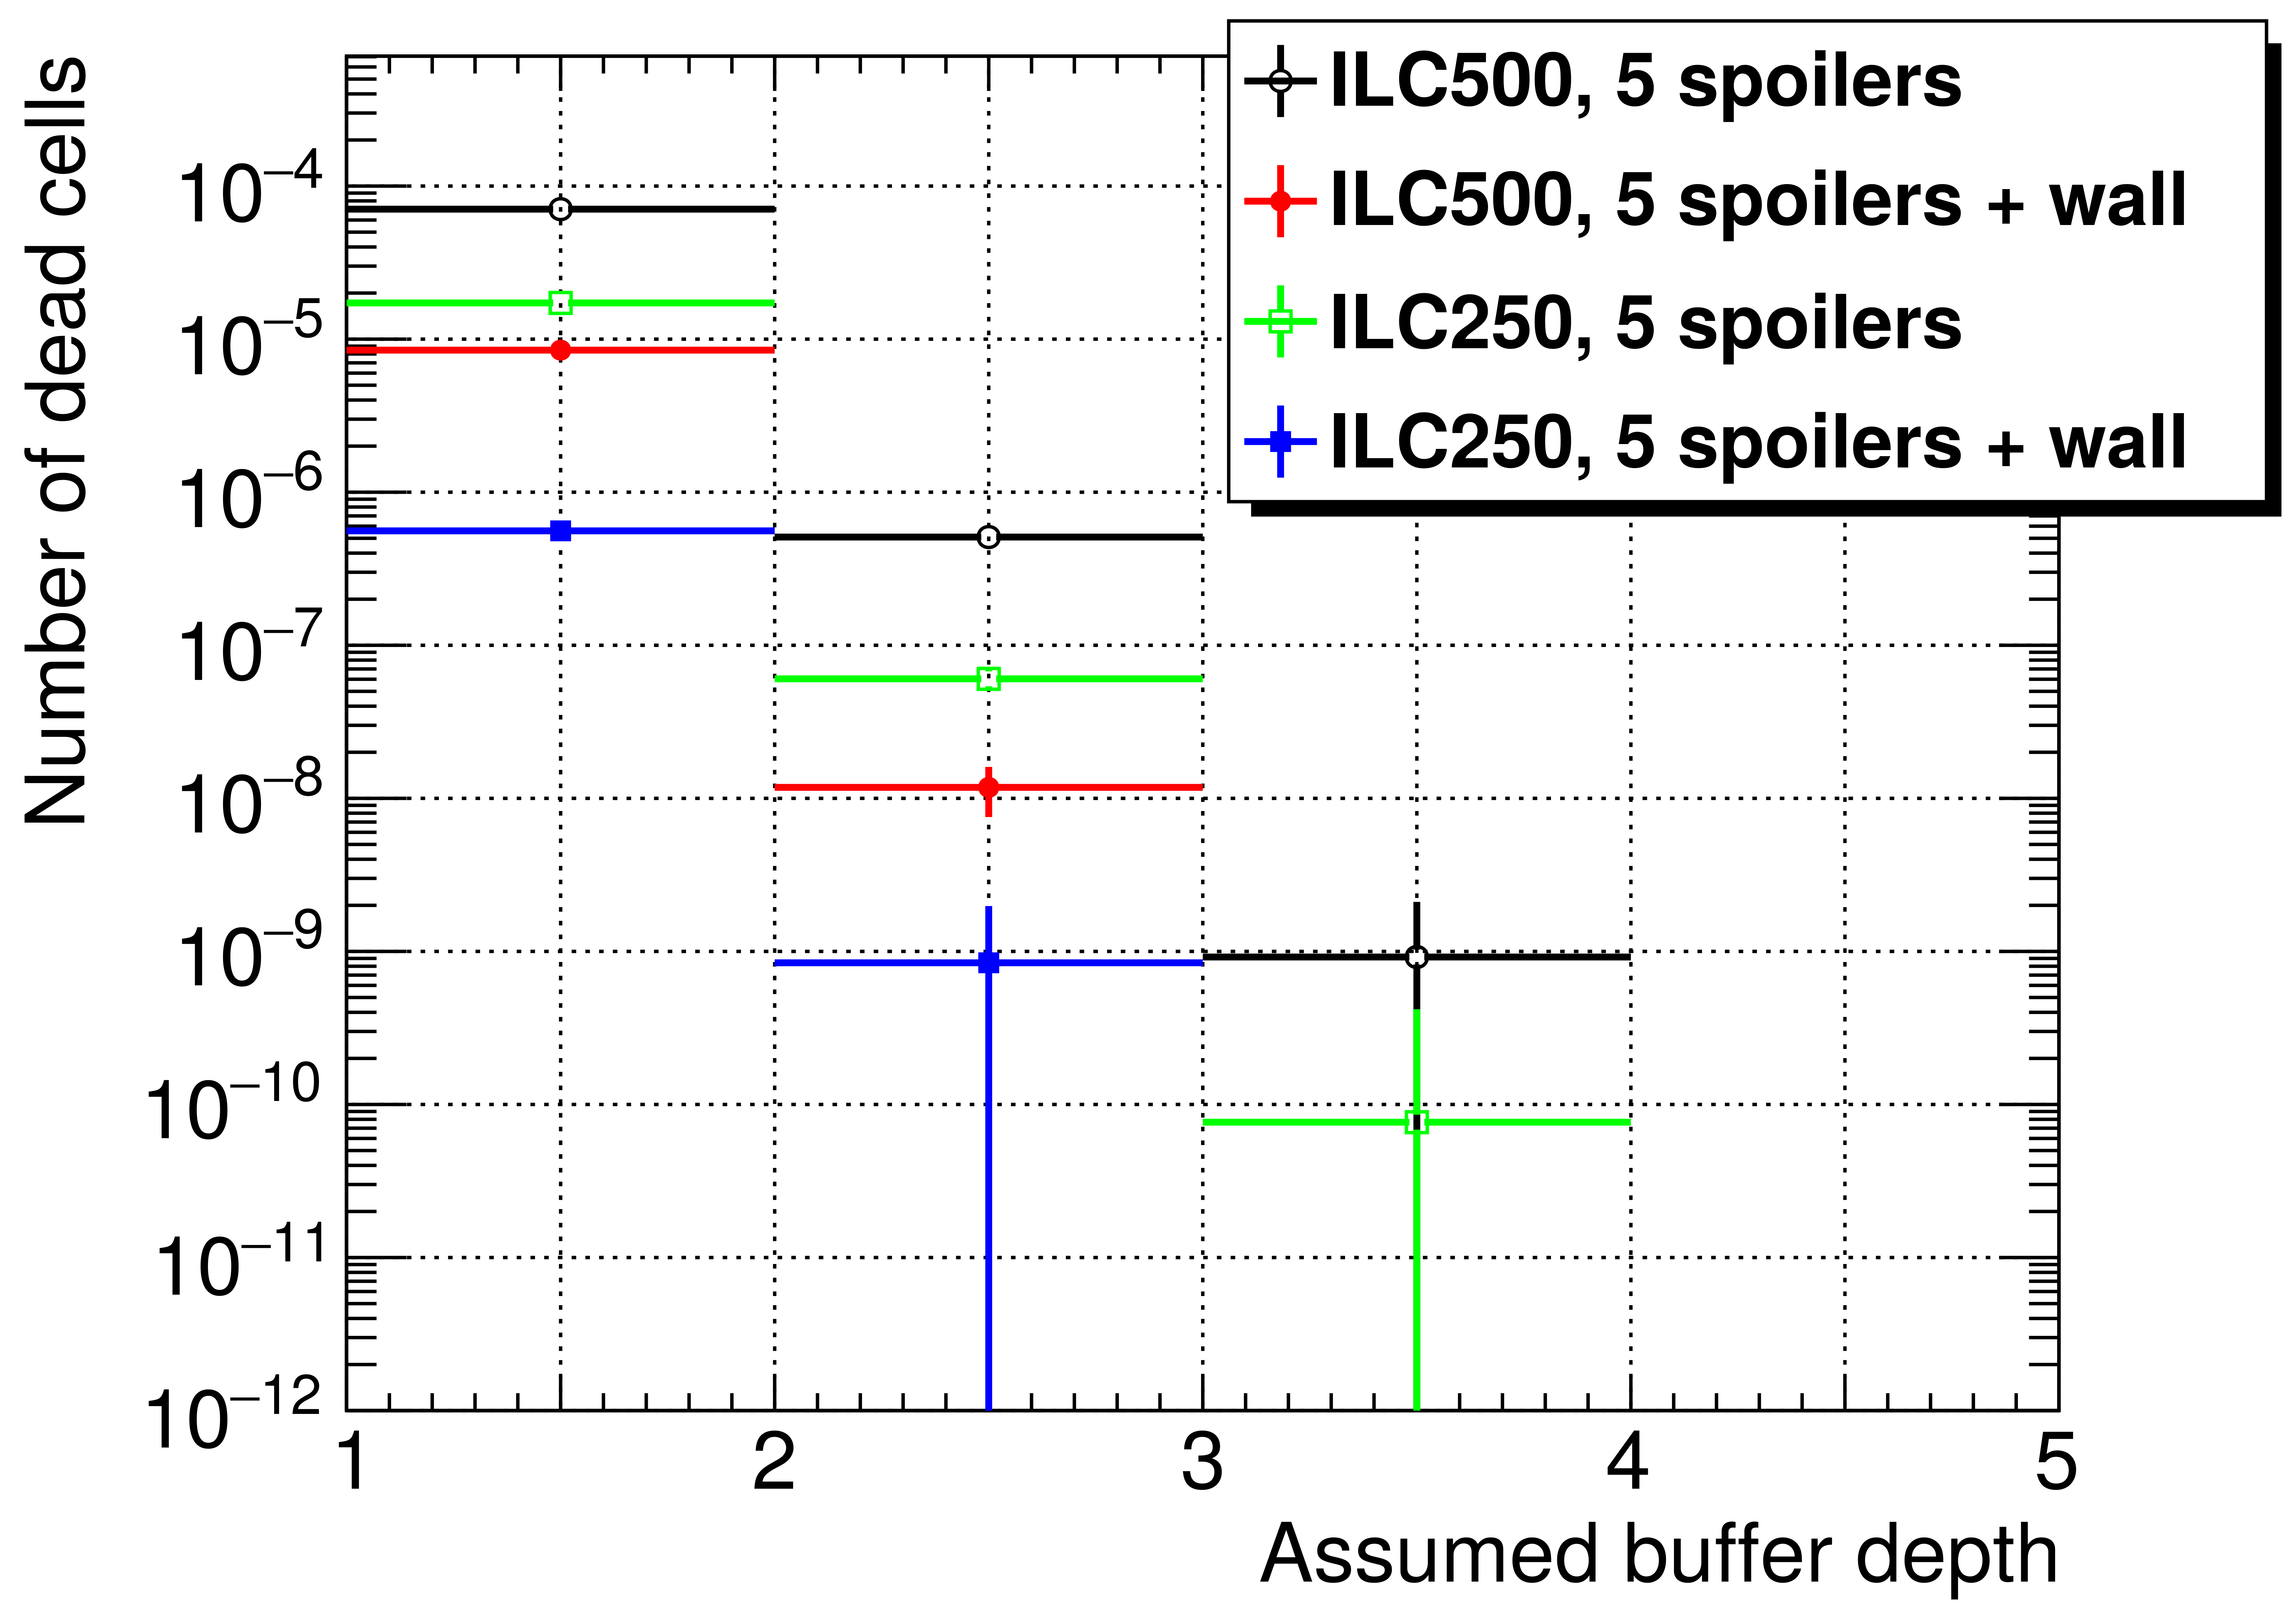
\includegraphics[width=\textwidth]{Figures/BDS_muons/Occupancy_Comparison_All_layers_deadcells_HcalBarrel.png}
   \caption{Normalized number of dead cells}
   \end{subfigure}
   \caption[\sid HCAL barrel occupancy from BDS muons]{Subfigure (a) shows the muon occupancy in the \sid HCAL barrel after a full bunch train, whilst subfigure (b) shows the number of dead cells resulting from this occupancy.
   Both histograms are normalized by the total number of cells in the HCAL barrel.
   The first bin of subfigure (a) contains the total number of cells, because of which the value of this bin is 1 for all cases.}
   \label{fig:BDS_Muons:HcalBarrel}
 \end{figure}
\\For the \sid tracker endcaps, however, the number of hits per cell reaches a maximum of 30 (see Figure~\ref{fig:BDS_Muons:SiTrackerEndcap}).
As for the \sid tracker, a readout cell size of \SI{50}{\micro\meter}$\times$\SI{50}{\micro\meter} was assumed, this is at first not to be expected.
The total number of hits in the tracker is smaller than in the HCAL, and yet the number of hits per cell reaches a much larger value.
The reason for this is that low energy (of the order of several hundred MeV) muons spiral in the magnetic field of the detector solenoid magnet, and by doing so hit the active layer of the tracker endcap several times.
An example of a loop performed by such a muon is depicted in Figure~\ref{fig:BDS_Muons:loop}.
Although the number of hits per cell ranges up to 30, the occupancy is consistently below \num{e-6} for all cases.
The number of dead cells, shown in Figure~\ref{fig:BDS_Muons:SiTrackerEndcap} (b), is plotted as a function of an assumed buffer depth of up to 30 accordingly.
Assuming the sensors in the \sid tracker will have a buffer depth of four, about \num{2e-8} of all cells would be dead for the ILC500 with the ``5 spoilers'' shielding only.
Also in this subdetector, the muon occupancy is below the critical limit for \sid for any buffer depth that might be chosen as the sensor design.
\\In the ILC500 stage, the occupancy for all subdetectors is reduced by at least a factor of five when adding a magnetized wall to the muon shielding.
This factor is even higher in the ILC250 stage.
Plots of the occupancy for the remaining \sid subdetectors can be found in Appendix~\ref{Appendix:BDS_Muons}.
  \begin{figure}
 \centering
  \begin{subfigure}[b]{0.49\textwidth}
   \centering
    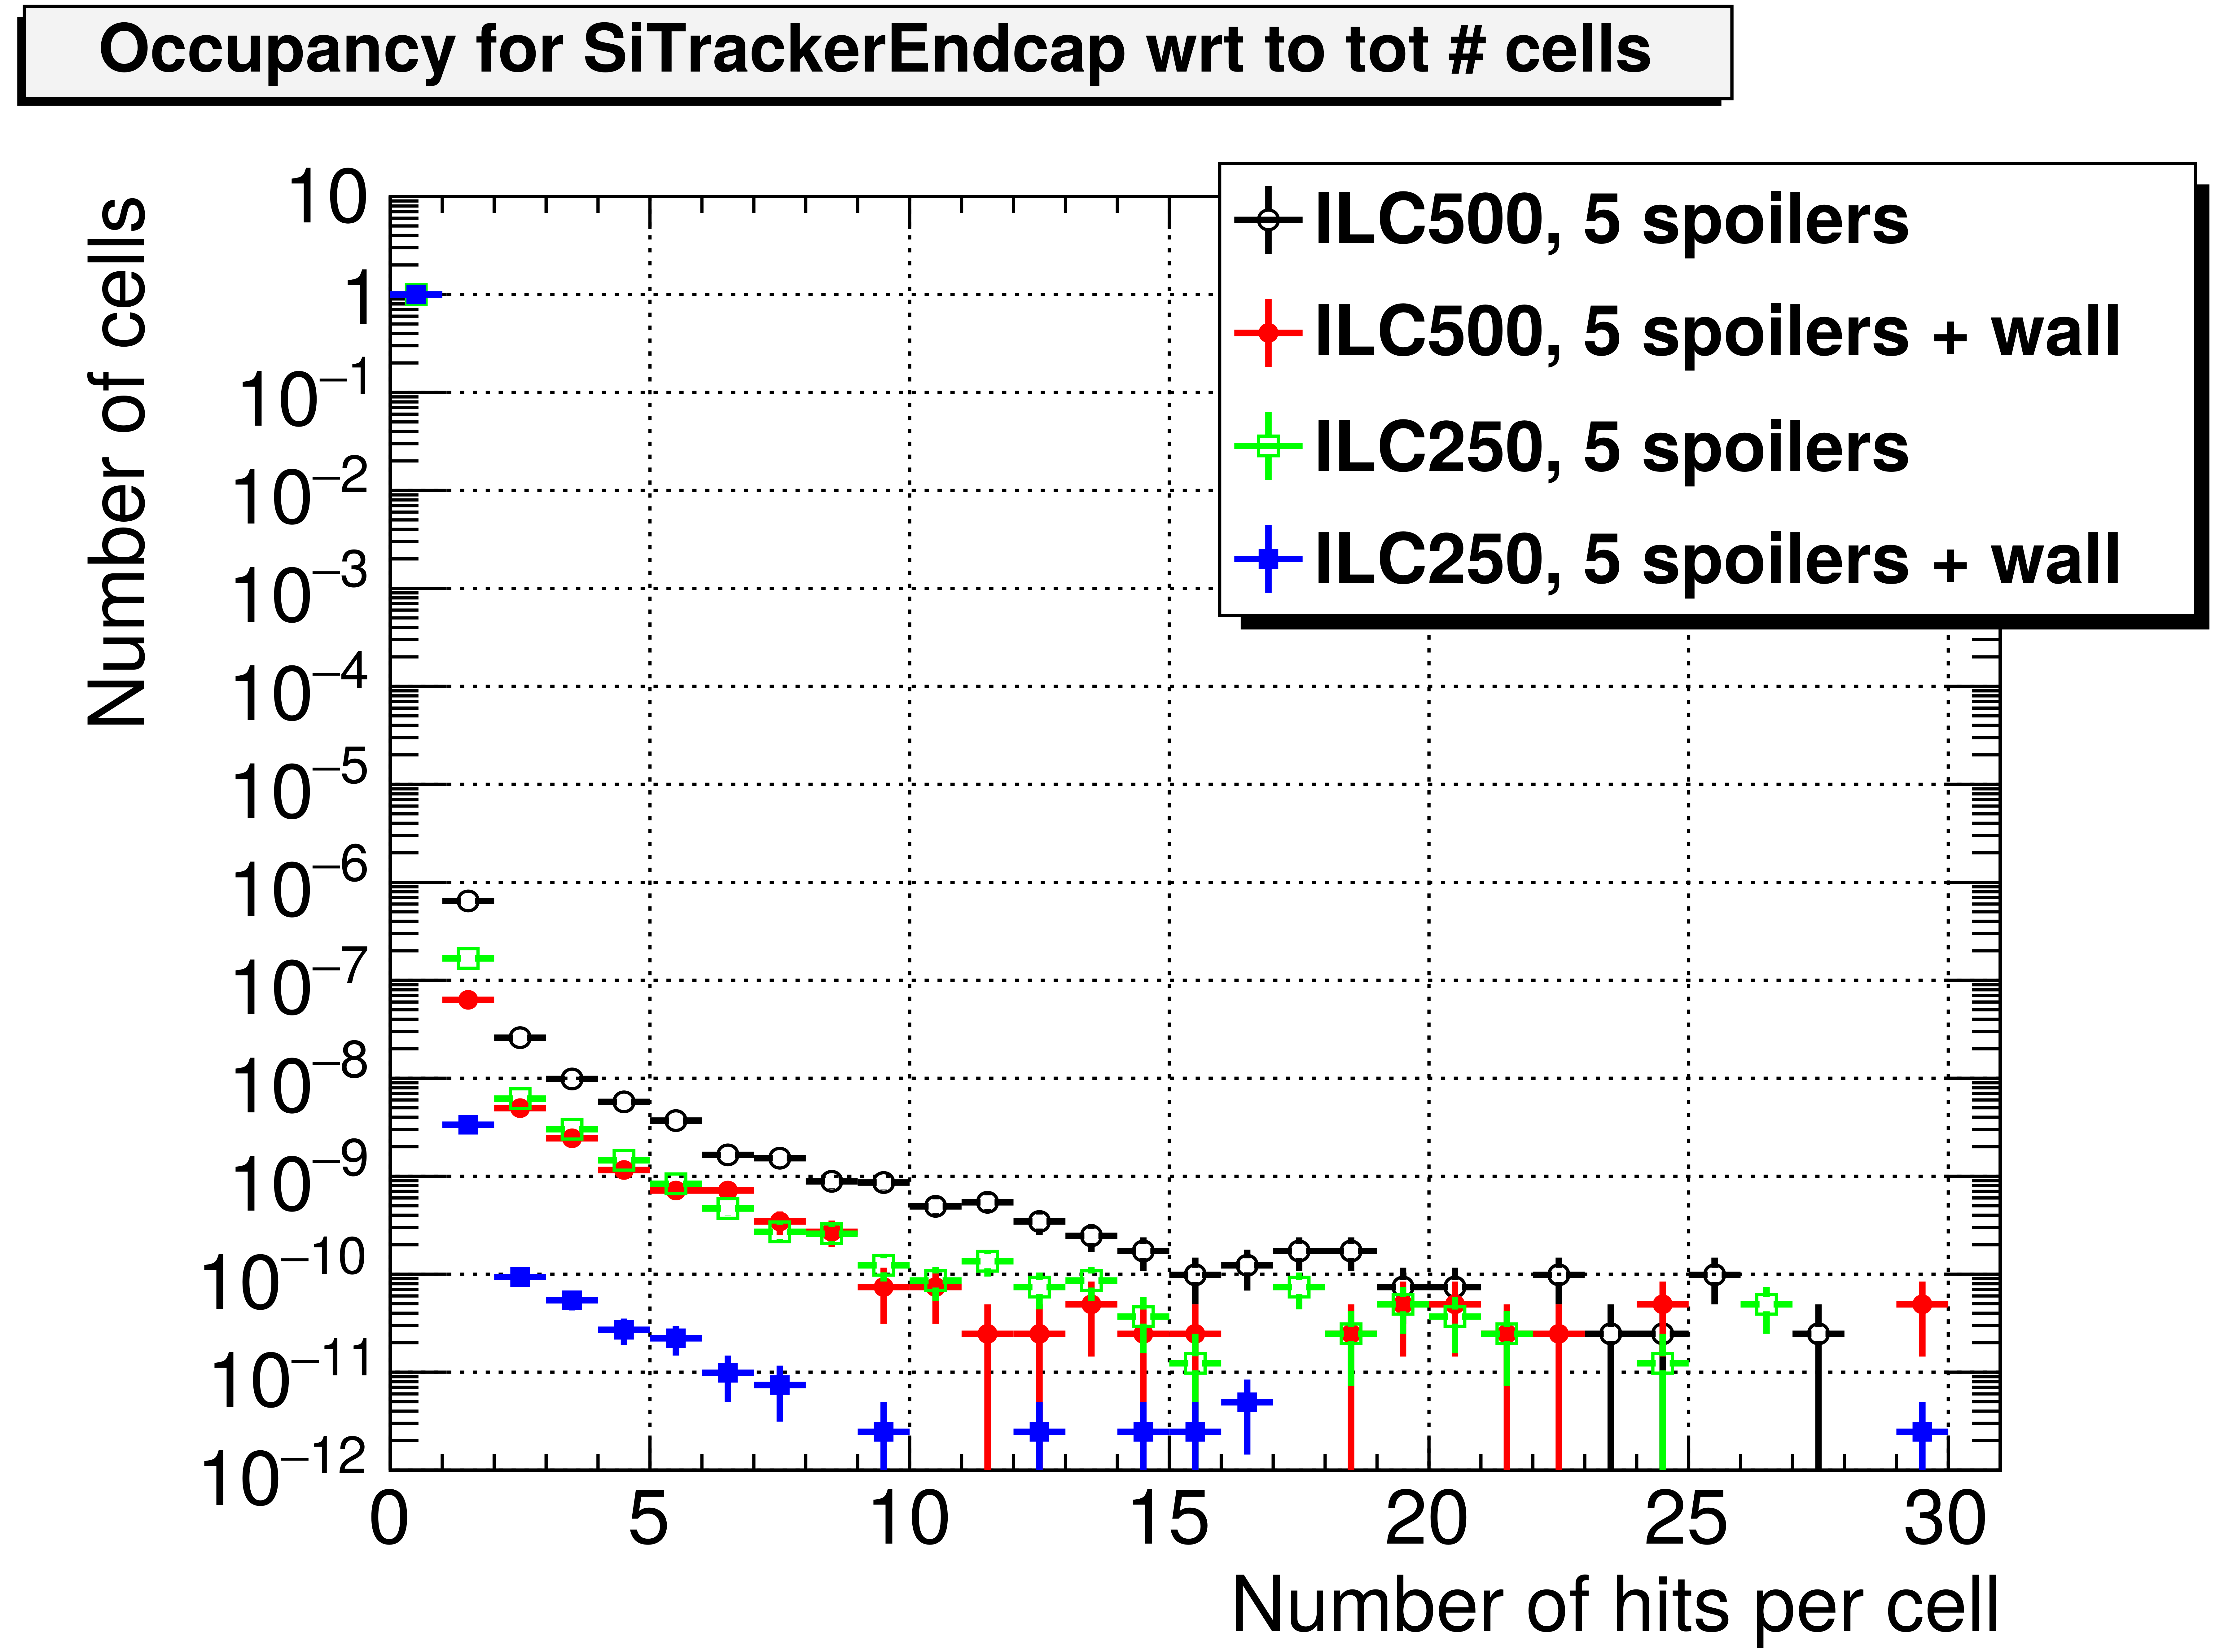
\includegraphics[width=\textwidth]{Figures/BDS_muons/Occupancy_Comparison_All_layers_wrt_cells_SiTrackerEndcap.png}
   \caption{Normalized occupancy}
   \end{subfigure}
   \hfill
    \begin{subfigure}[b]{0.49\textwidth}
   \centering
    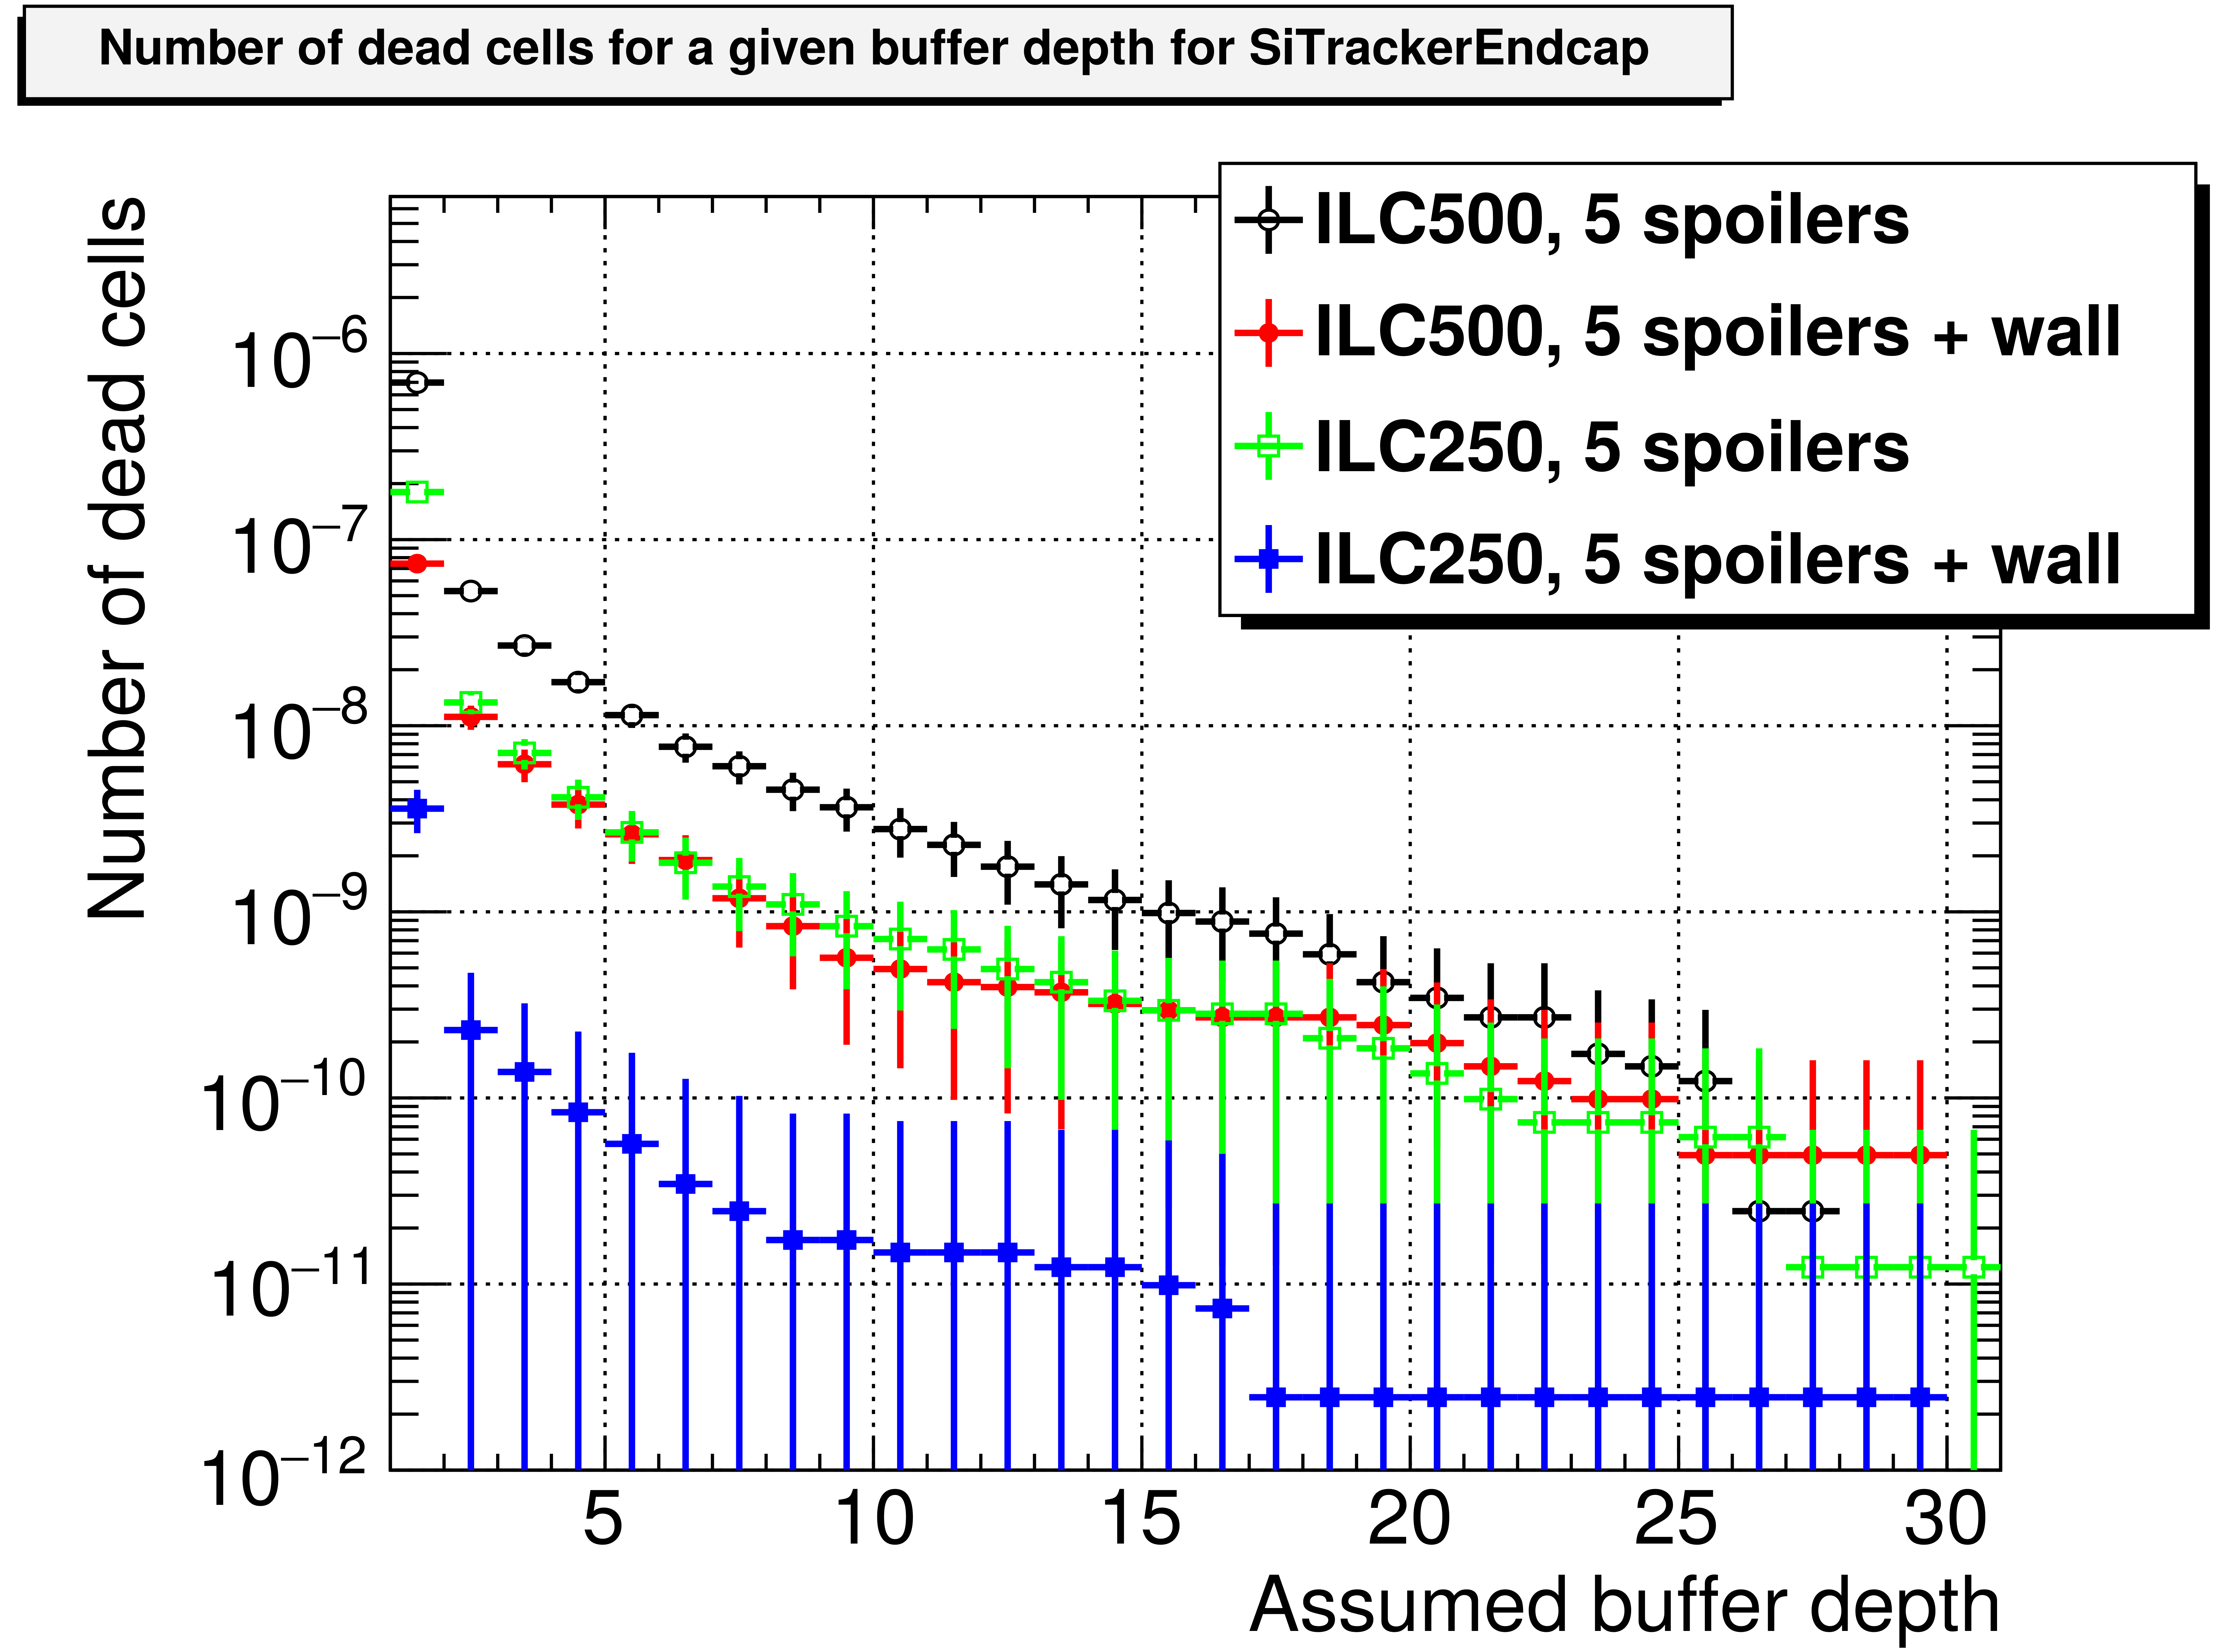
\includegraphics[width=\textwidth]{Figures/BDS_muons/Occupancy_Comparison_All_layers_deadcells_SiTrackerEndcap.png}
   \caption{Normalized number of dead cells}
   \end{subfigure}
   \caption[\sid tracker endcap occupancy from BDS muons]{Subfigure (a) shows the muon occupancy in one of the \sid tracker endcaps after a full bunch train, whilst subfigure (b) shows the number of dead cells resulting from this occupancy.
   Both histograms are normalized by the total number of cells in the tracker endcap.
   The first bin of subfigure (a) contains the total number of cells, because of which the value of this bin is 1 for all cases.}
   \label{fig:BDS_Muons:SiTrackerEndcap}
 \end{figure}
 
 \begin{figure}[htbp!]
\centering
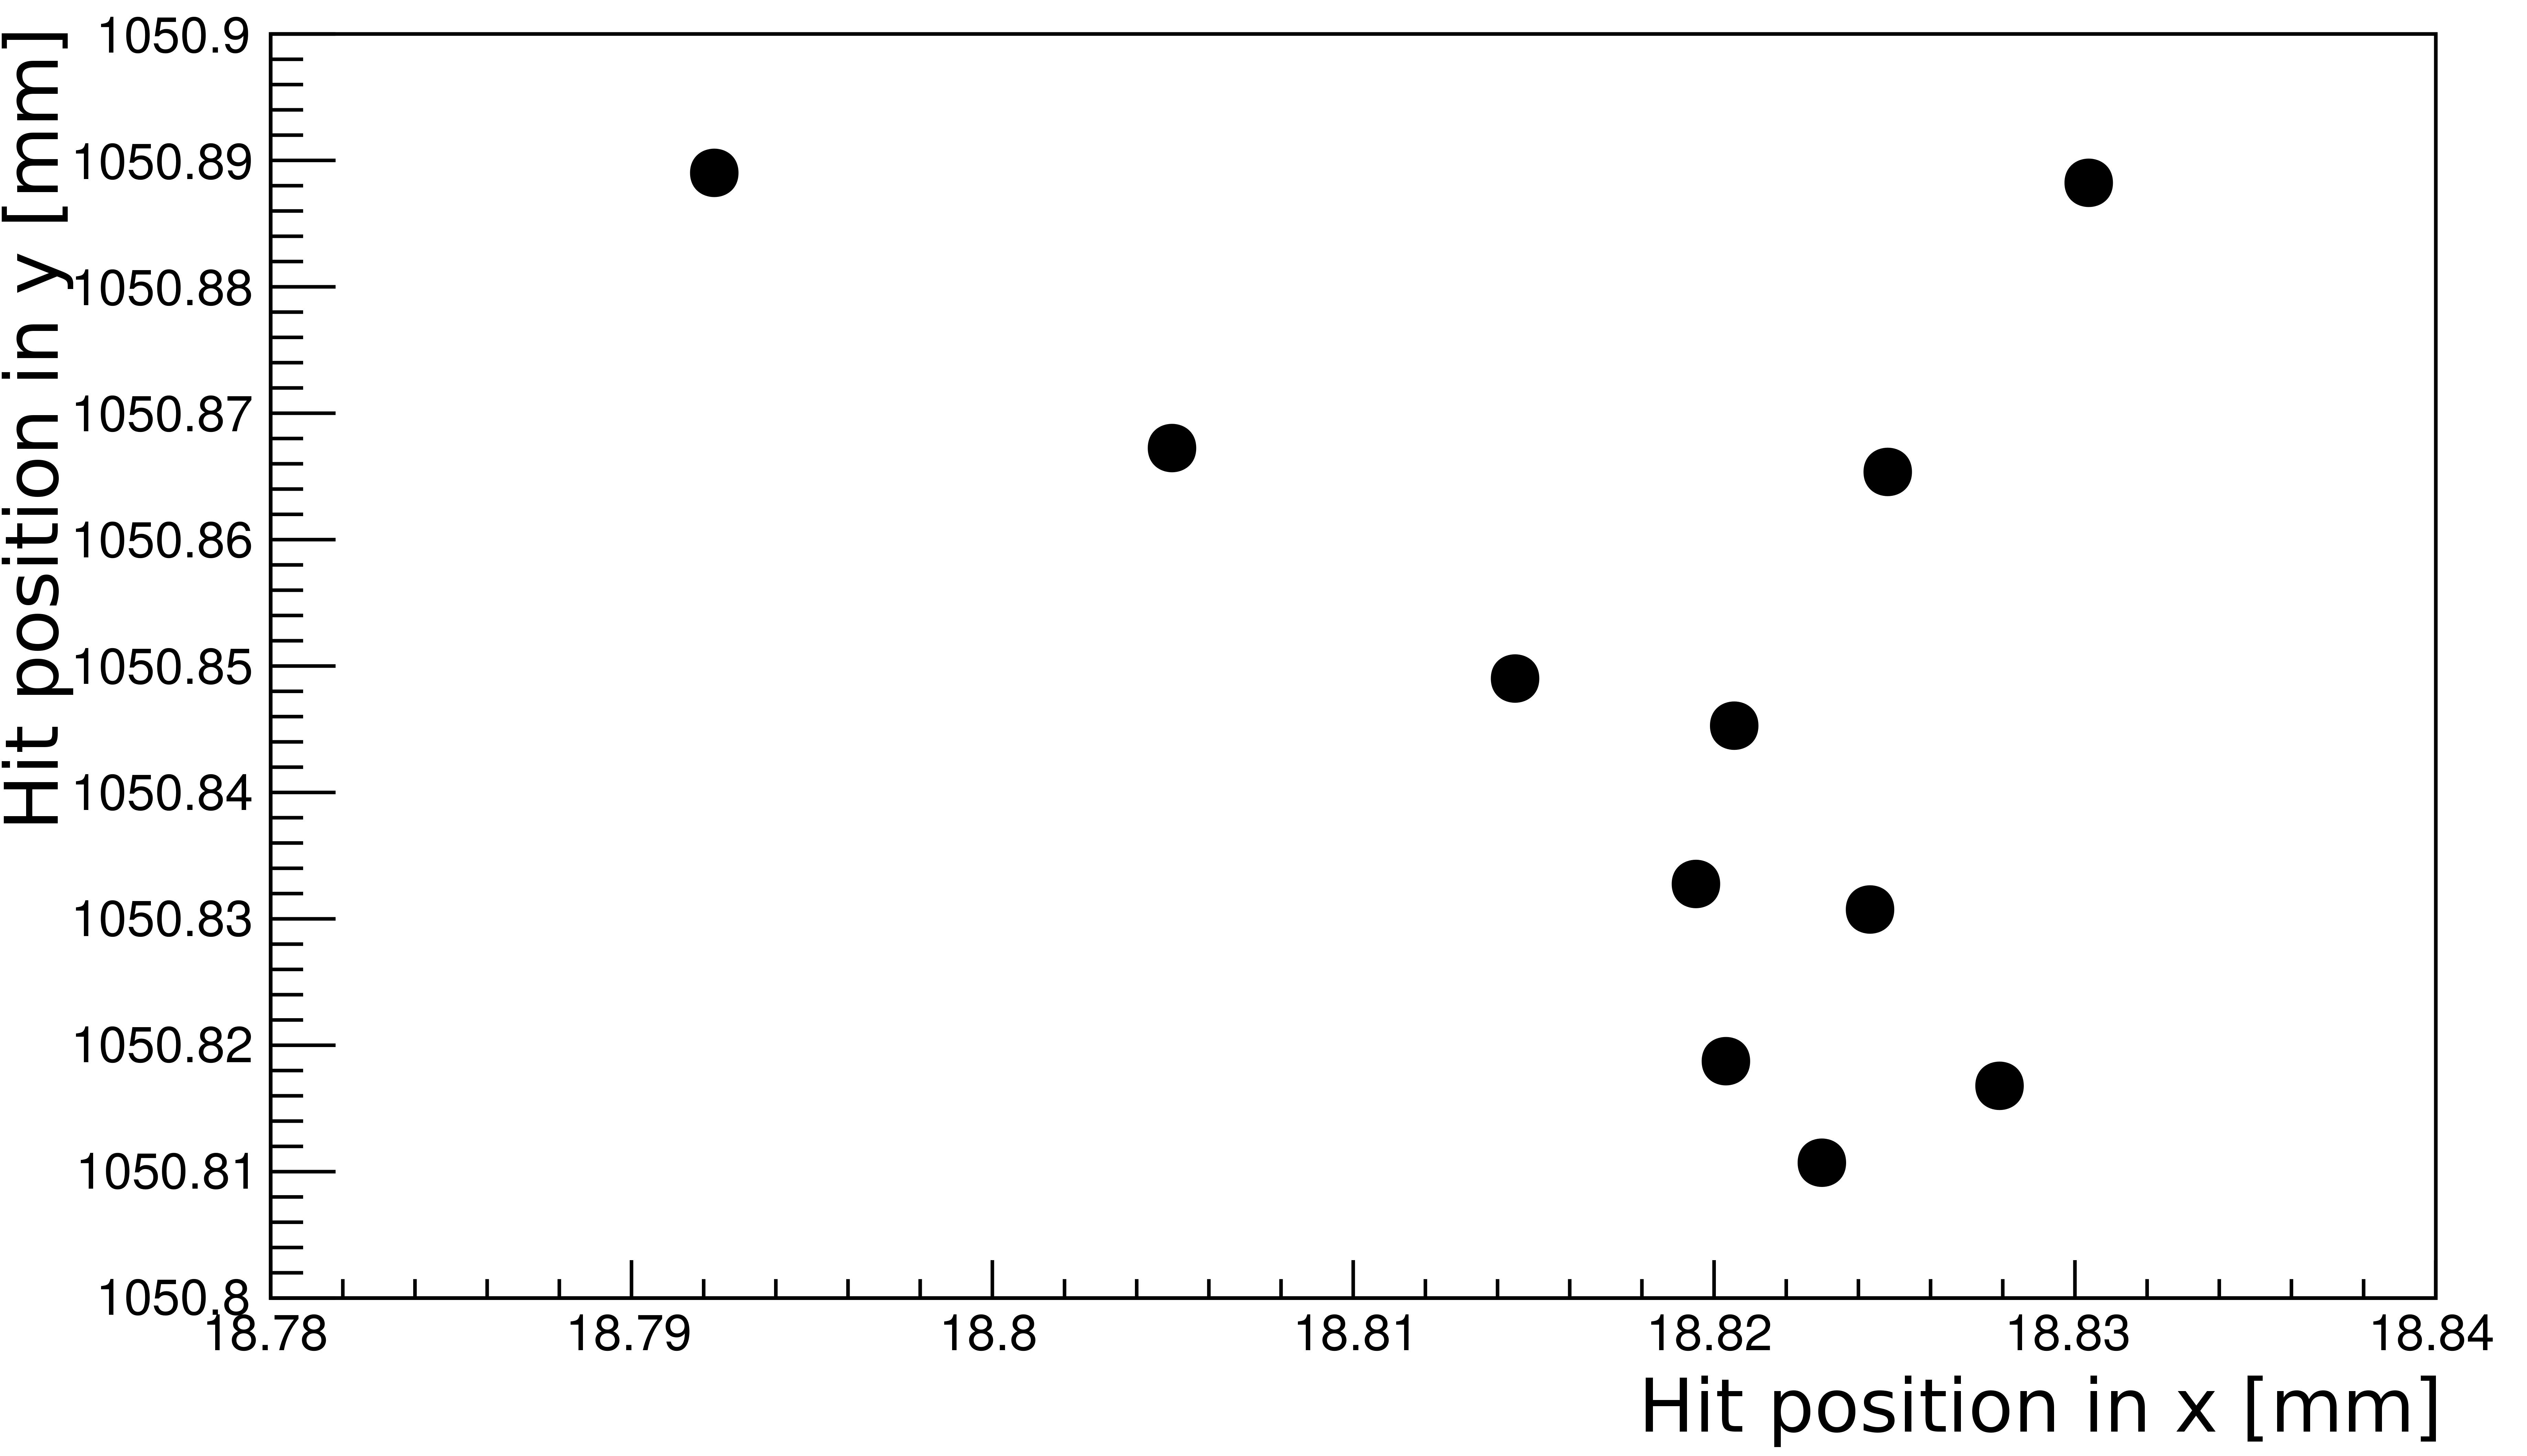
\includegraphics[width=0.5\textwidth]{Figures/BDS_muons/LoopInACell.png}
\caption[BDS muons looping]{Hit position of muon hits in the \sid tracker endcap, in layer number four.}
\label{fig:BDS_Muons:loop}
\end{figure}

\subsection{Conclusion}
This section presented a study of the effect of the muons from the BDS on the \sid occupancy for two different shielding options.
For the first option, five magnetized spoilers would be installed at different locations along the beam line.
For the second option, a magnetized wall would be placed between these spoiler locations and the interaction region, as an additional shielding device.
The comparison of the occupancy in these two cases revealed that the magnetized wall reduces the occupancy by a significant amount.
Nevertheless, the occupancy level is in both cases far from the critical limit of \num{e-4}, which is especially important in the tracking systems of the \sid detector.
For these subdetectors, a minimal background occupancy is crucial to guarantee a high performance in the track reconstruction of physics events.
For a center-of-mass energy of \SI{250}{\GeV} in the first ILC stage, the \sid tracker endcap occupancy for an assumed buffer depth of four is about \num{4e-9} for the minimal shielding option without the wall.
Since in the next ILC stage at a center-of-mass energy of \SI{500}{\GeV}, the number of muons reaching the detector is larger by a factor of three, also the occupancy for the same buffer depth is increased by about a factor of three for the ``5 spoilers'' case.
However, it still does not exceed \num{e-7}.
\\Overall, the magnetized wall does not seem to be necessary in order to limit the muon occupancy in \sid, for both studied center-of-mass energies.
However, the wall serves as a tertiary containment device against muons and other machine background particles.
The decision might be to keep the wall anyway for the protection of personnel and maintenance staff, depending on the restrictions imposed by radiation safety regulations.
A solution to lessen the price for the wall would be to change its design such that its thickness is reduced and it is not magnetized.
The wall would then still serve as additional shielding but does not deflect charged particles. \\An idea for future studies of the muon shielding would be to also adjust the detector specific Pacman design with respect to different materials and the possibility of magnetizing the Pacman volume.

%---------------------------------------------------
\section{Beam halo collimators in the Final-Focus system}

The Final-Focus (FF) system is responsible for focusing the ILC beam to nanometer size, as explained in Section~\ref{ILC:layout}. 
By decreasing the beam size, the aim of reaching high luminosities can be achieved.
%The reason behind this is the aim \todo{requirement?} for high luminosities, which can be gained by small beam sizes.
In order to reduce the machine background arising from interactions of the beam with the Final-Focus components, beam halo collimators will be installed that cut off the halo around the beam core. 
\\For testing the feasibility of such collimators for future linear colliders such as the ILC, a vertical beam halo collimator has been installed at the \mbox{Accelerator Test Facility 2} (ATF2)~\cite{ATF} at the High Energy Accelerator Research Center Organization (KEK) in Japan~\cite{Nuria_Thesis}. 
In March 2016, data of the background in the proximity of the collimator were taken in dependency of the aperture of this collimator. 
This section covers the analysis of the data as well as simulation studies done with \bdsim.

\subsection{The Accelerator Test Facility 2}
\label{ATF2}

The Accelerator Test Facility 2 (ATF2) is an extension to the accelerator facility ATF at the High Energy Accelerator Research Center Organization (KEK) in Japan~\cite{ATF}. 
As can be seen in Figure~\ref{fig:ATF}, ATF consists of a linear accelerator, which pre-accelerates electrons to \SI{1.3}{\GeV} before they enter the damping ring. 
\\ATF2 is a test bench for the FF system of the ILC and has two main goals: 
\begin{enumerate}
 \item Focusing the low-emittance beam to \SI{37}{\nano\metre} in the vertical plane
 \item Demonstrating the stability of the nanometer sized beam at the interaction point
\end{enumerate}
So far, focusing the beam to a size of \SI{40}{\nano\metre} has been shown to be repeatable. 
Although the beam size goal of ATF2 seems to be large compared to the ILC goal of \SI{9}{\nano\metre}, the ATF2 system is directly comparable to the ILC Final-Focus system. 
The beam size goal has to be scaled up for different lattice and beam conditions.\\
\begin{figure}
\centering
\includegraphics[width=\textwidth]{Figures/ATF/ATF.png}
\caption[ATF accelerator]{A schematic of the ATF accelerator with the ATF2 extension~\cite[cf. p. 65]{Nuria_Thesis}.
ATF consists of a linear accelerator, a damping ring, the new ATF2 extension with the Final-Focus system, and a beam dump.}
\label{fig:ATF}
\end{figure}
Additionally, as the ATF serves as a research accelerator, the ATF collaboration allows research groups to test new accelerator and diagnostic components, to operate the accelerator themselves, and to take measurements for their research.
ATF therefore offers a unique opportunity for young researchers to conduct their experiments and to gain experience in operating a particle accelerator.
\\To this end, the vertical beam halo collimator, which was proposed and designed for reducing the machine background at linear colliders, was installed in ATF2 in the beginning of March 2016 by Nuria Fuster-Martinez~\cite{Nuria_Thesis}. 
In a collaboration of Ph.D. students, valuable experience was gained working together with Nuria Fuster-Martinez in the installation and operation of diagnostic hardware for particle detection, and in the operation of the ATF beam.
Whilst the focus of her research was the construction and installation of the collimator, as well as the measurements of its general functionality, the focus for this part of the thesis at hand was independent measurements of background particles in the proximity of the collimator.
\\The vertical beam halo collimator and the Cherenkov detector, with which the background level was measured in dependency of the collimator aperture, are both located in the FF section of ATF2. 
A schematic of the ATF2 lattice with the collimator and the Cherenkov detector is shown in Figure~\ref{fig:ATF2}. 
The Cherenkov detector was built and setup by a group from the Royal Holloway University of London (RHUL)~\cite{RHUL_detector_wiki}, because of which the detector is in the following sections referred to as the ``RHUL Cherenkov detector''.
A more detailed description of this detector is given in Section~\ref{RHUL}.
\begin{figure}
\centering
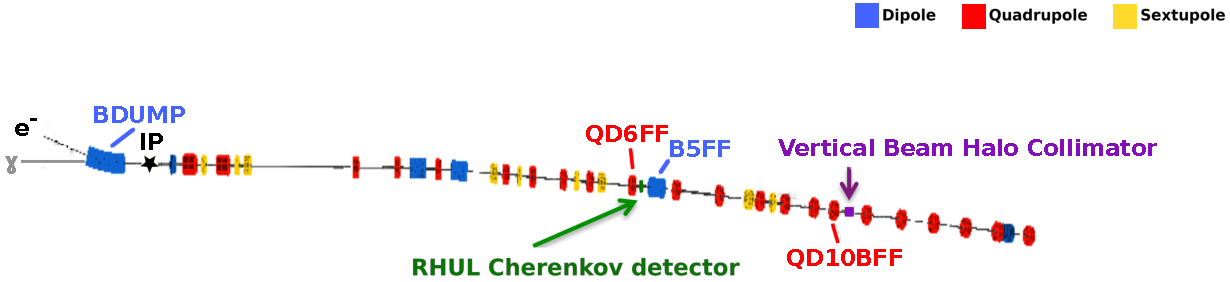
\includegraphics[width=\textwidth]{Figures/ATF/ATF2schematic.pdf}
\caption[ATF2 schematic]{A schematic of the ATF2 lattice~\cite{Nuria}. 
The beam direction is from right to left. 
The beam halo collimator is located before the quadrupole magnet `QD10BFF', the Cherenkov detector is installed downstream between the dipole magnet `B5FF' and the quadrupole magnet `QD6FF'. 
After the interaction point (IP), the electron beam is bent in the last dipole magnet `BDUMP' towards the beam dump. 
}
\label{fig:ATF2}
\end{figure}

\subsection{Vertical beam halo collimator}
\label{Collimator}

The purpose of the vertical beam halo collimator is to cut off the beam halo in the vertical direction, in order to reduce the machine background at the IP.
The design drawings of the collimator structure are shown in Figure~\ref{fig:collimator}.
The collimating jaws are inside a structure that is evacuated and connected to the beam pipe of the ATF2 beam line. 
A picture of the installed collimator is given in Figure~\ref{fig:installed_collimator}.
The actual jaws are made of copper, the other components of stainless steel. 
The jaws have an overall length of \SI{238}{\milli\meter}, and a cross-sectional area of \mbox{\SI{24}{\milli\meter}$\times$\SI{24}{\milli\meter}}.
They can be moved individually to an arbitrary position inside the possible range, so that the inner edge of the jaws can have a distance of between 2.6 and \SI{12}{\milli\metre} to the center. 
The full aperture of the collimator structure can therefore be between 5.2 and \SI{24}{\milli\metre}. 
The error on the position of the jaws is about \SI{10}{\micro\metre}.\\
As every component in a beam line, especially for such small beam sizes, is affecting the electromagnetic field of the passing beam, the collimator is designed to minimize the effect of inducing wakefields~\cite{NuriaCollimator2015,Nuria_Thesis}. 
This thesis, however, focuses exclusively on the effect on the background level, as mentioned above.
\begin{figure}
\centering
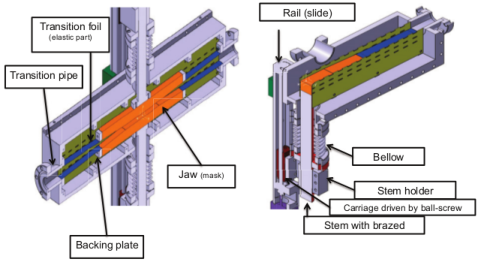
\includegraphics[width=0.8\textwidth]{Figures/ATF/ATF2_beamhalo_collimator.pdf}
\caption[Drawing of the beam halo collimator]{A drawing of the vertical beam halo collimator installed at ATF2.~\cite{NuriaCollimator2015}}
\label{fig:collimator}
\end{figure}
\begin{figure}
\centering
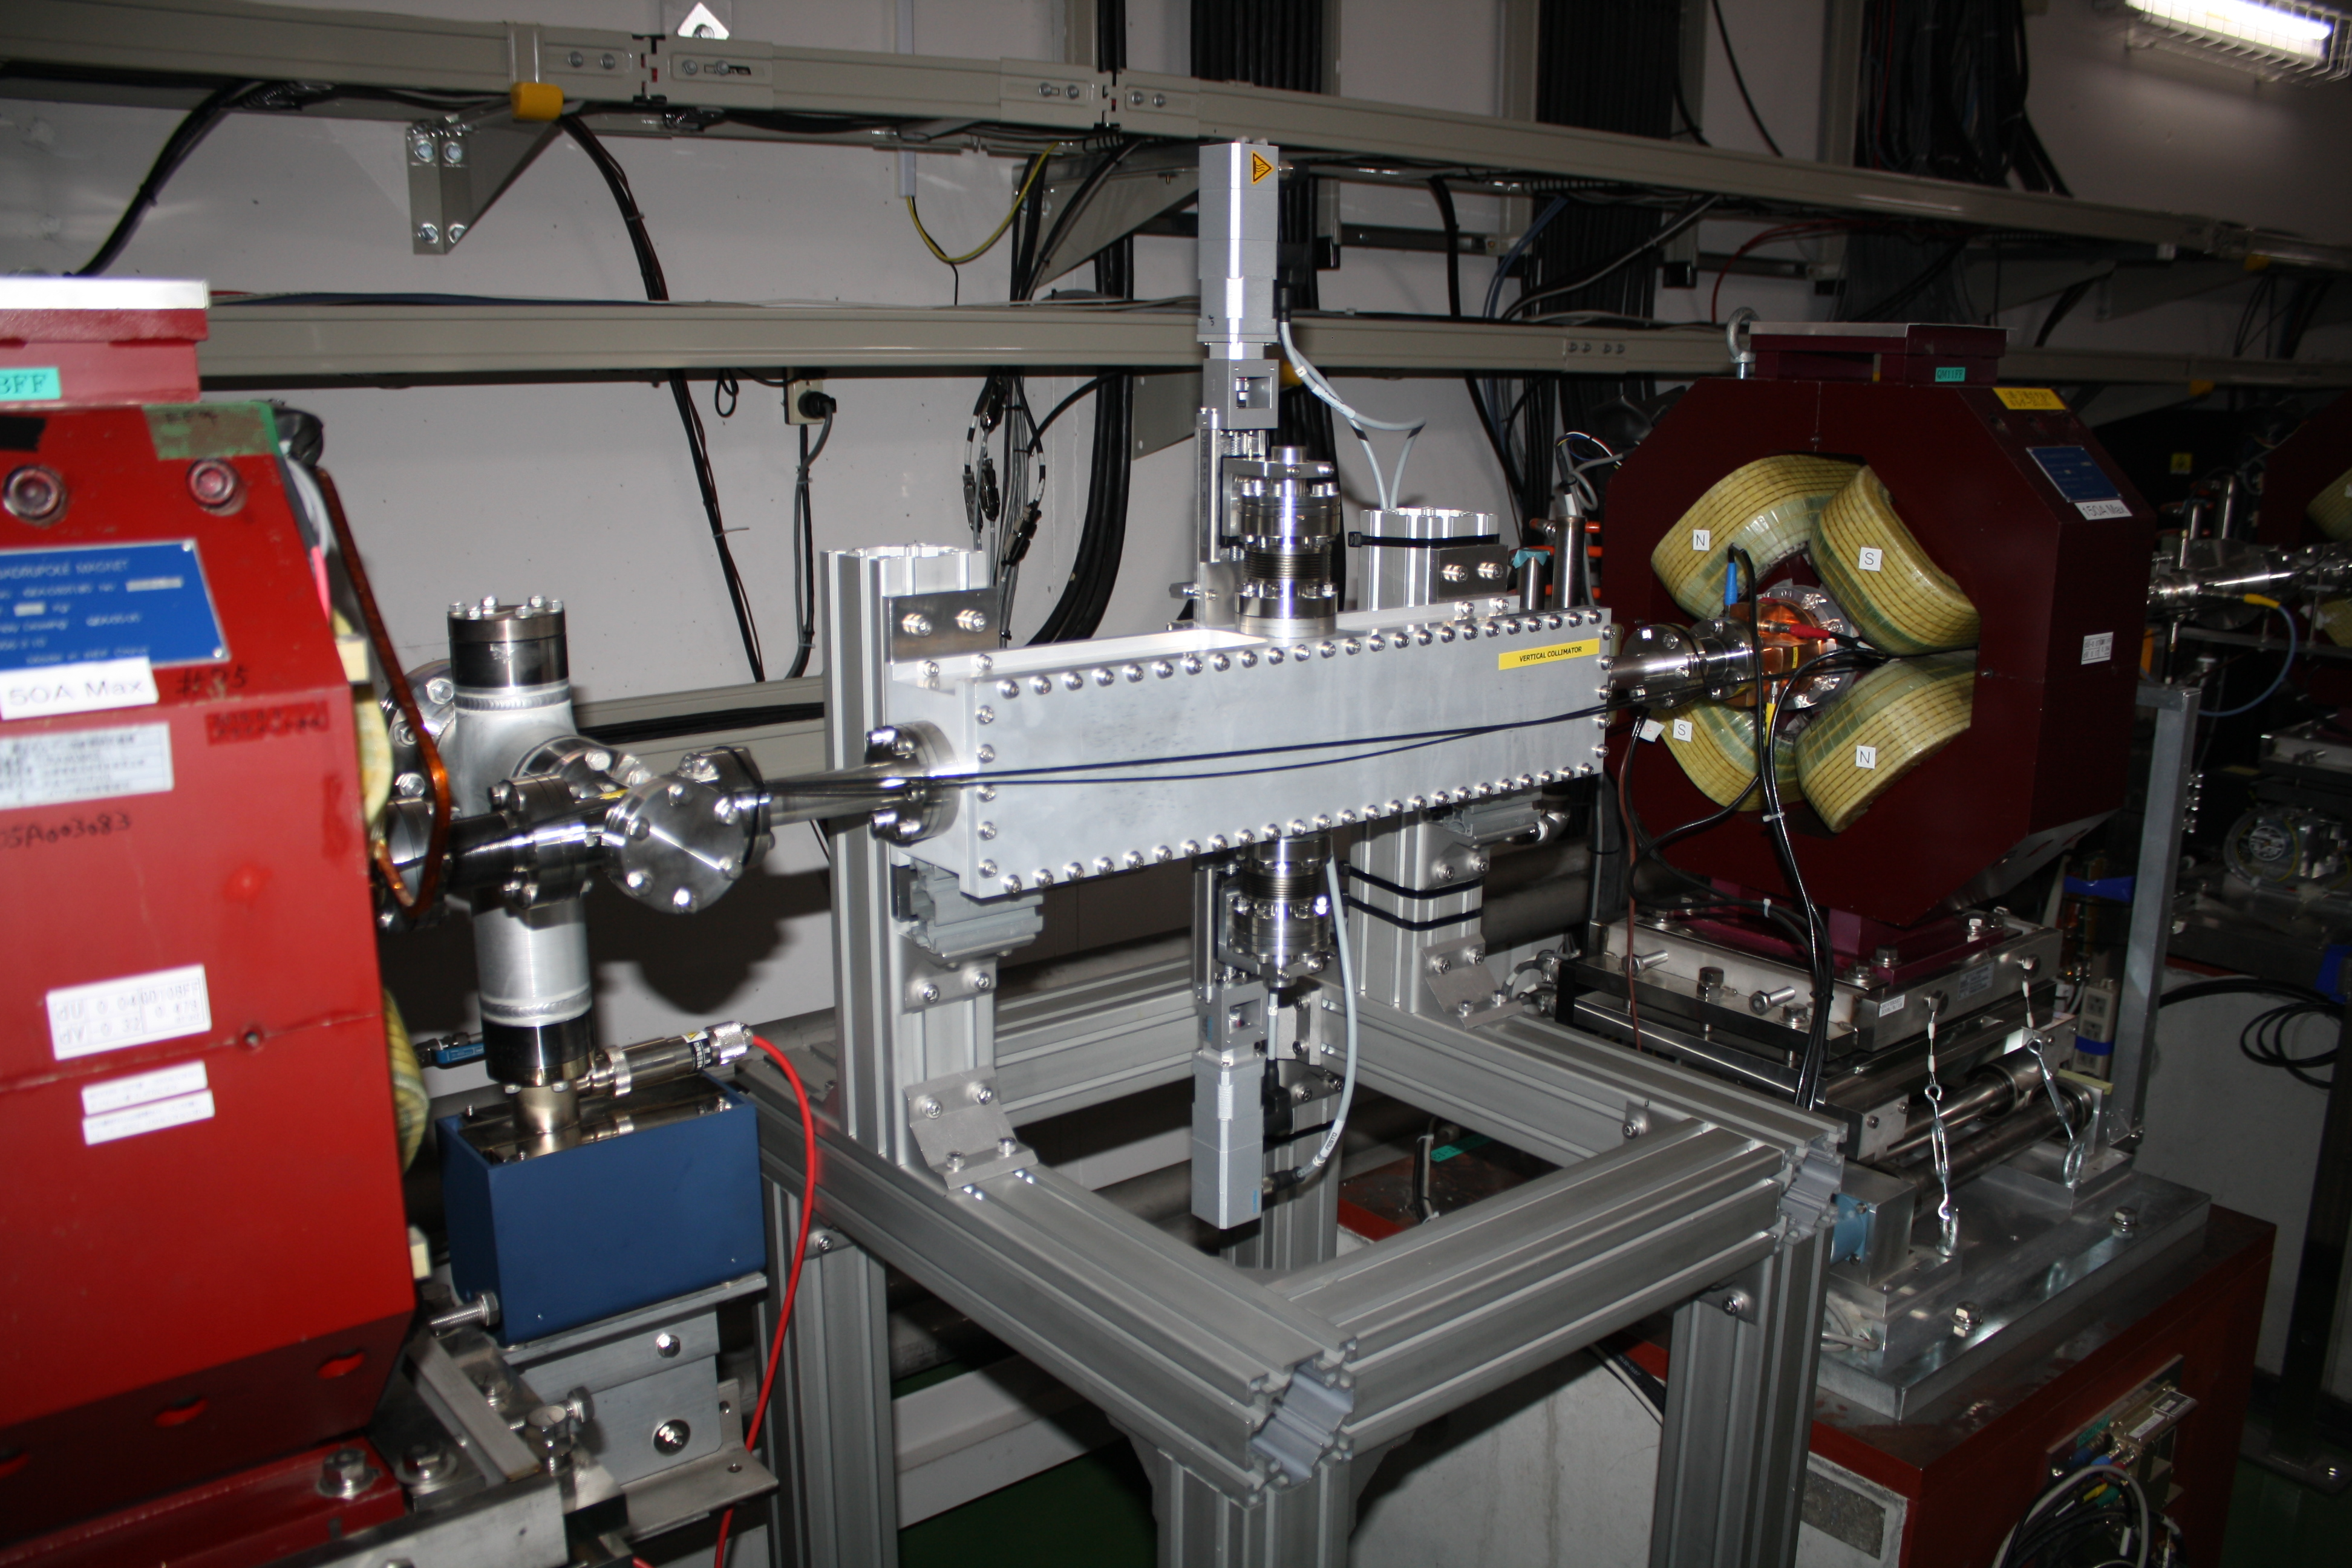
\includegraphics[width=0.8\textwidth]{Figures/ATF/Installed_Collimator.jpg}
\caption[Picture of the installed beam halo collimator]{A picture of the vertical beam halo collimator built into ATF2. 
The collimator jaws are within the evacuated structure. 
At the top and bottom of the structure, the mover system for the two jaws can be seen.}
\label{fig:installed_collimator}
\end{figure}

%---------------------------------------------------
\subsection{Background studies}
\subsubsection{RHUL Cherenkov detector}
\label{RHUL}

The RHUL Cherenkov detector~\cite{RHUL_detector_wiki} uses the Hamamatsu photomultiplier tube (PMT), which was previously installed in a laserwire sensor that was located at the same position in the ATF2 beam line. 
The Cherenkov detector itself is using aerogel\footnote{SP15, index 1.015, 4 slices, \SI{4}{\centi\meter\squared}, \SI{5}{\centi\meter} deep} as its radiator medium. 
A light-guiding pipe, with a profile area of \SI{10}{\centi\metre\squared} and a total length of \SI{35}{\centi\metre}, directs the light from the aerogel to the PMT.
Figure~\ref{fig:RHUL_Cherenkov_Drawing} shows a schematic drawing of the detector setup.
Pictures taken of the detector at the ATF2 beam line are shown in Figure~\ref{fig:RHUL_Cherenkov}.
\\It is installed downstream of a dipole magnet, which deflects the beam electrons along the beam line.
Photons from particle showers, however, are not deflected and continue along a straight line.
The entrance of the Cherenkov detector is positioned such that these neutral secondary particles can be detected.
The beam electrons are deflected past the detector.
The detected photons are an indication of the particle showers produced by interactions between the beam and the beam line components.

\begin{figure}
\centering
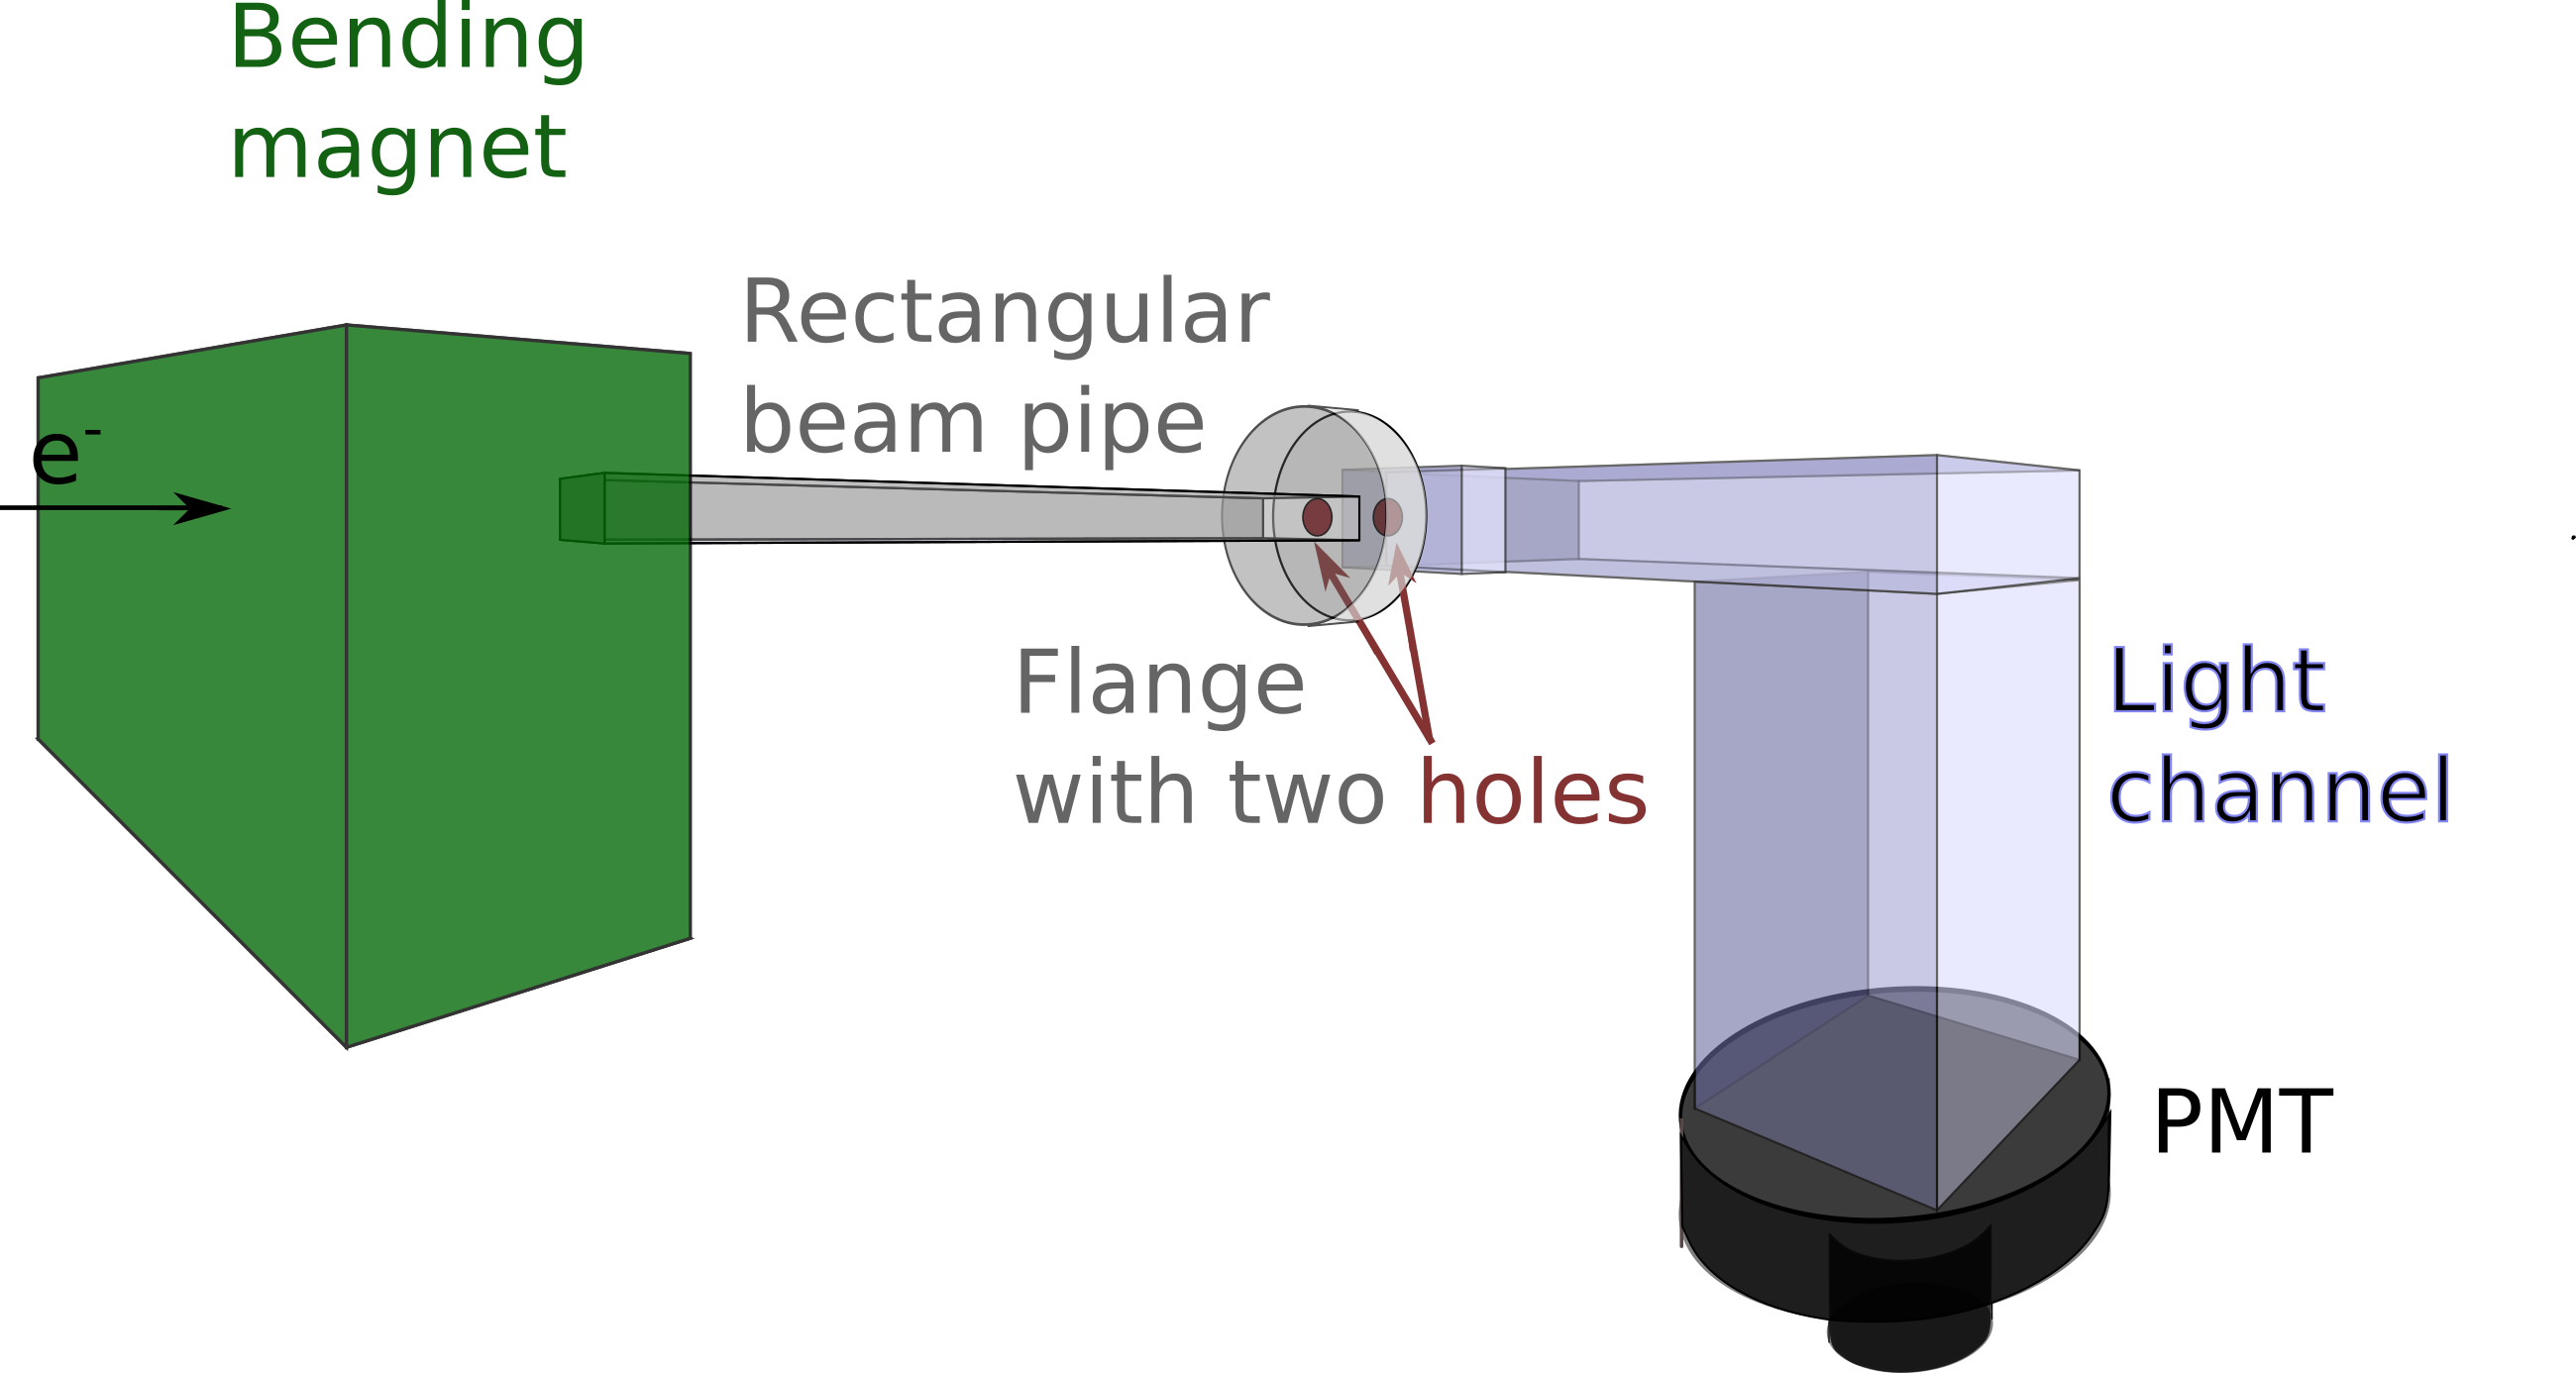
\includegraphics[width=0.8\textwidth]{Figures/ATF/drawing_CherenkovSetup.png}
\caption[Schematic drawing of the RHUL Cherenkov detector setup]{A perspective schematic of the RHUL Cherenkov detector setup in ATF2.
The beam electrons are bent in the dipole magnet, and continue through the rectangular beam pipe along the ATF2 beam line, and past the RHUL Cherenkov detector face.
The neutral particles on the other hand, which are not deflected in the magnetic field, continue along a straight line through the rectangular beam pipe, and enter the RHUL Cherenkov detector through the second window in the flange. 
The light signals are collected by the PMT.}
\label{fig:RHUL_Cherenkov_Drawing}
\end{figure}

\begin{figure}
\begin{center}
\resizebox{.9\textwidth}{!}{%
\includegraphics[height=0.35\textheight]{Figures/ATF/CherenkovDetector_inBeamLine1.png}%
\quad
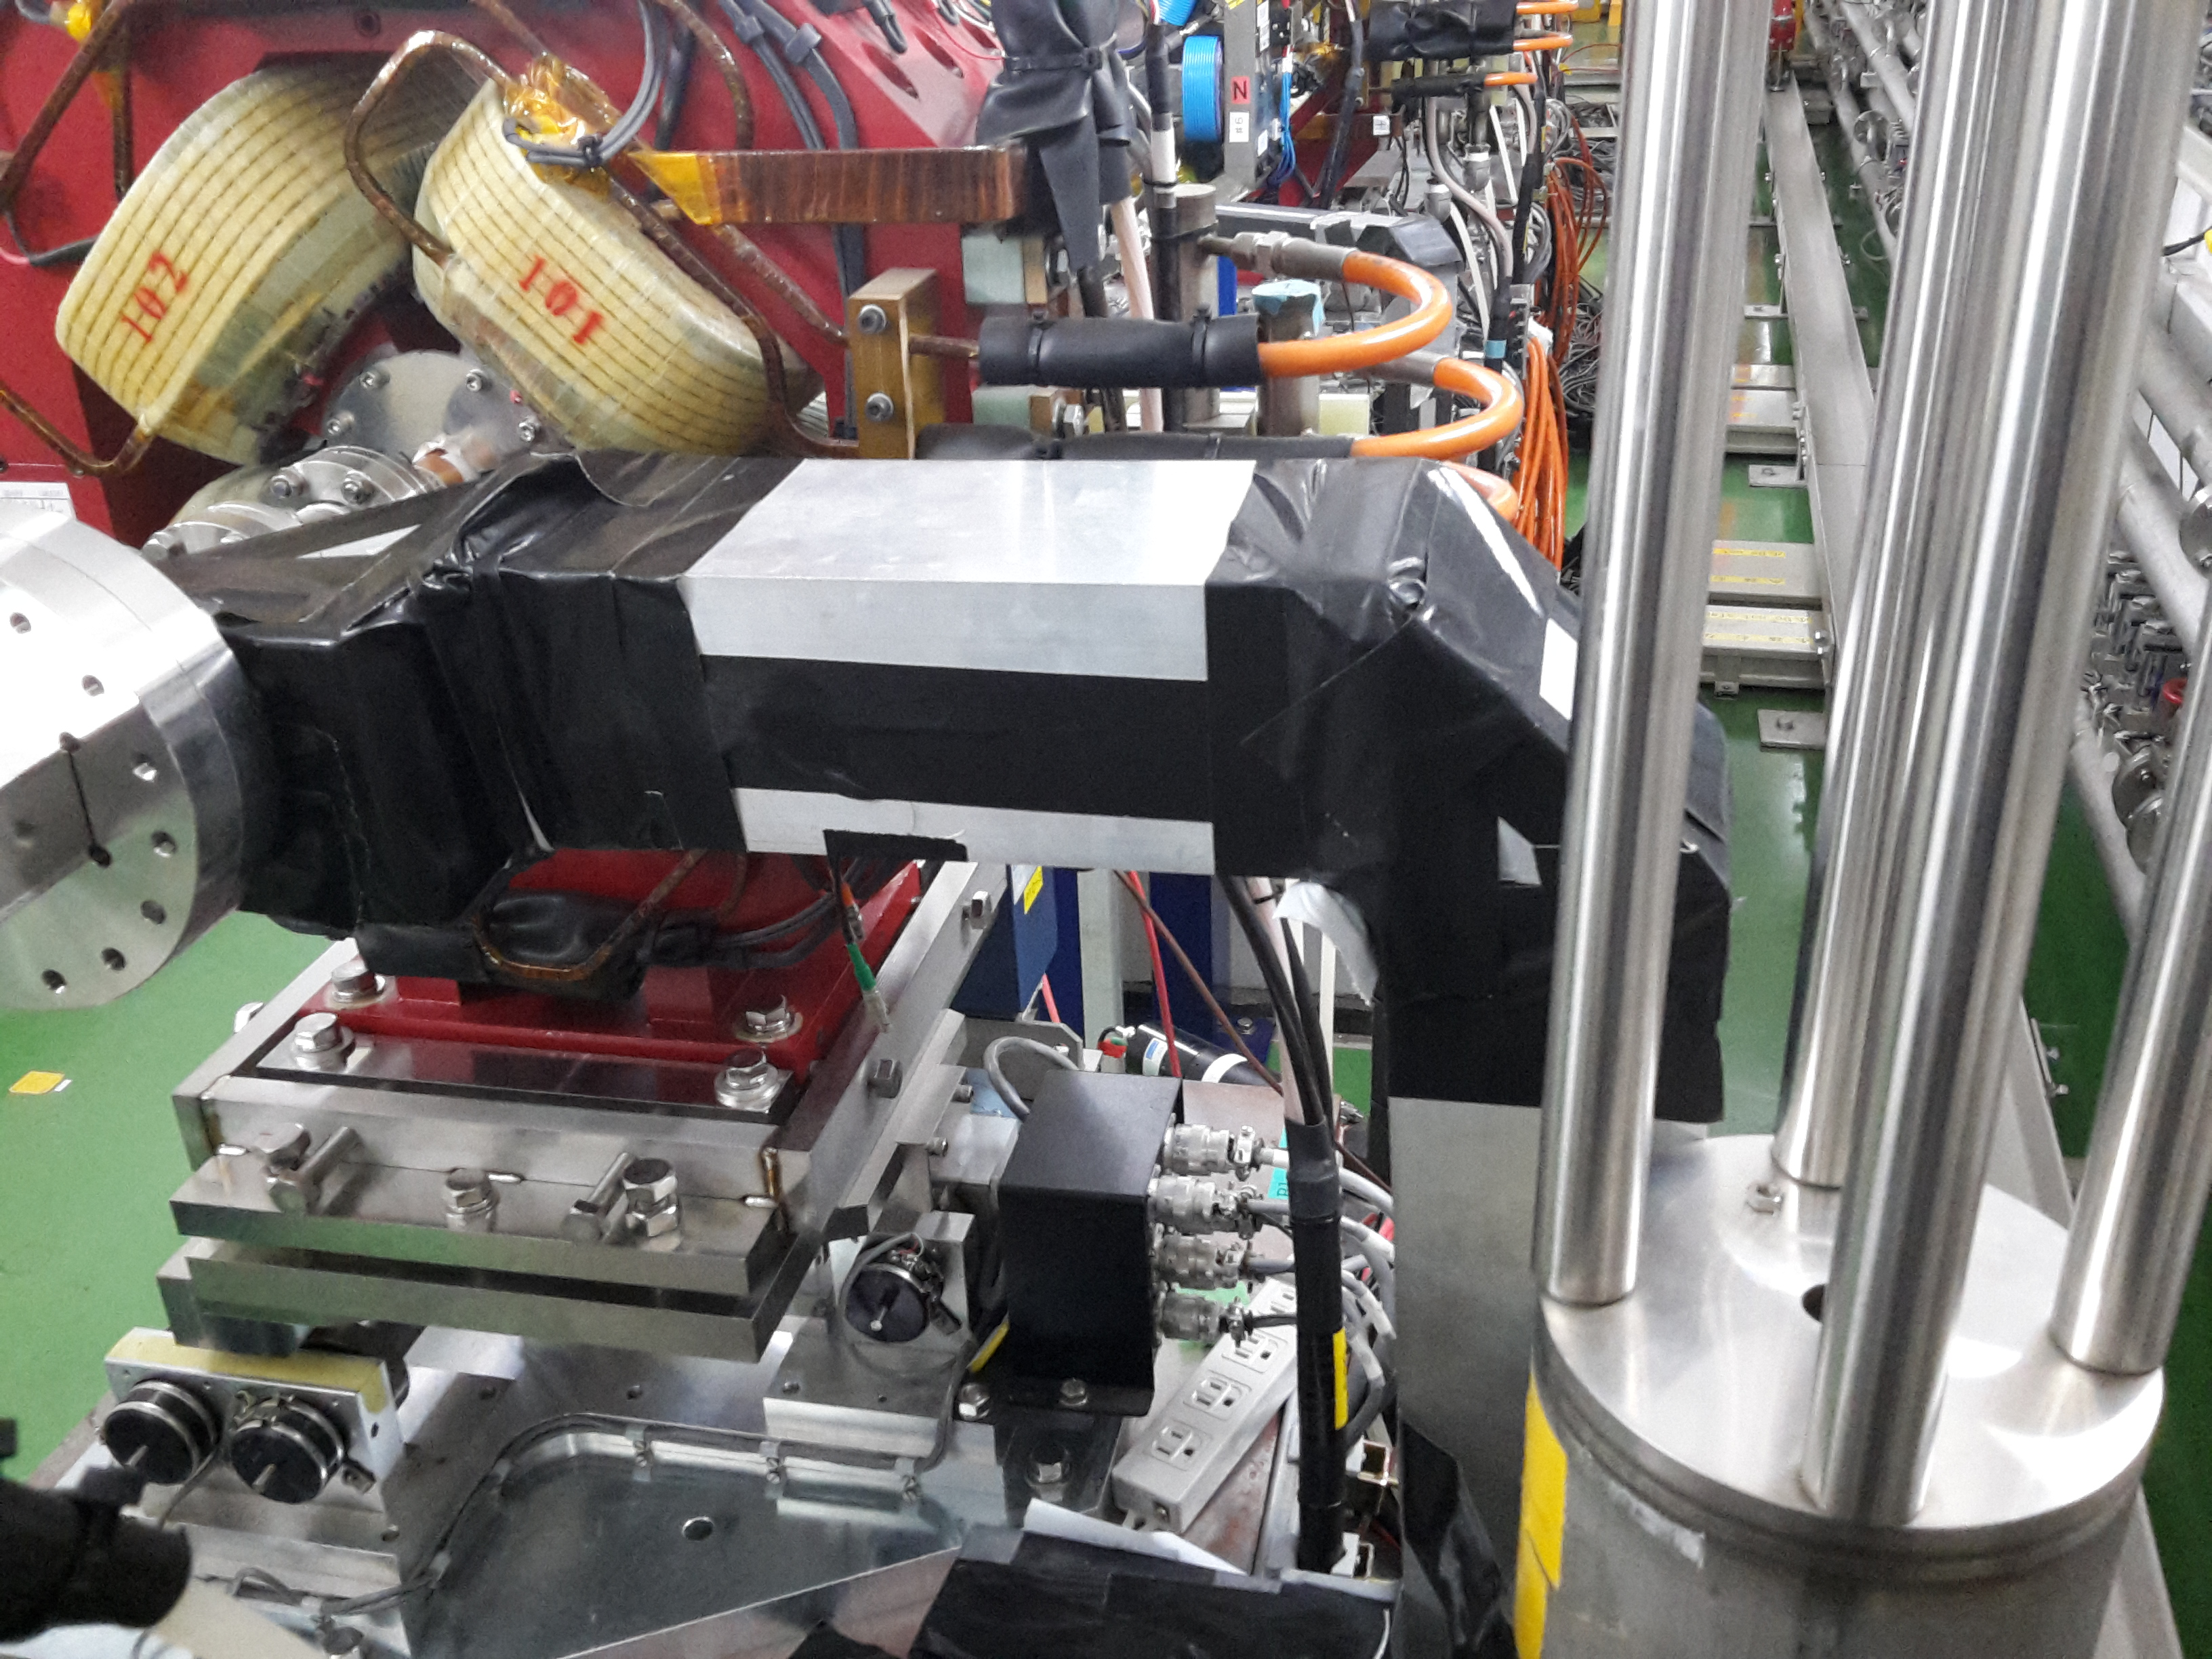
\includegraphics[height=0.35\textheight]{Figures/ATF/CherenkovDetector_inBeamLine2.jpg}%
}
\caption[Pictures of the RHUL Cherenkov detector]{Pictures of the RHUL Cherenkov detector in ATF2. 
The aerogel detector and the light channel are positioned behind a flange that connects the rectangular beam pipe with a circular one. 
The flange has two openings, one for the circular beam pipe, another one covered by a plastic window through which the photons leave the rectangular beam pipe and enter the RHUL Cherencov detector.}
\label{fig:RHUL_Cherenkov}
\end{center}
\end{figure}

\paragraph{PMT noise measurements}
Before measurements of the shower particles could be taken, the PMT noise had to be measured.
The noise is the signal that is measurable by the PMT, when the beam is turned off.
Figure~\ref{fig:AverageNoise_VoltageNormalization} (a) shows the mean values of the noise measurements for different PMT voltages. 
For every point either 500 or 1000 ADC pulses were recorded and averaged.
The error bars represent the standard deviation on the mean value calculated with \mbox{$SD=\frac{\sigma}{\sqrt{N}}$}, where $\sigma$ is the RMS of the noise distribution at each point and N the number of pulses.\\
At around \SI{800}{\volt}, the effect of dark current in the PMT becomes prominent, because of which the noise rises exponentially. 
Some of the possible causes of dark current are:
the thermionic emission of electrons from the photocathode and the dynodes, leakage current between the anodes and cathodes, and ionization current from residual gases inside the PMT~\cite[p. 67]{Hamamatsu}.
\\As the data was taken only for the voltages for which noise measurements were done, the mean value of noise is subtracted from every signal pulse appropriately. 
Therefore, the rise in noise is automatically taken into account for higher voltages.
\begin{figure}
\centering
\begin{subfigure}[b]{0.49\textwidth}
 \centering
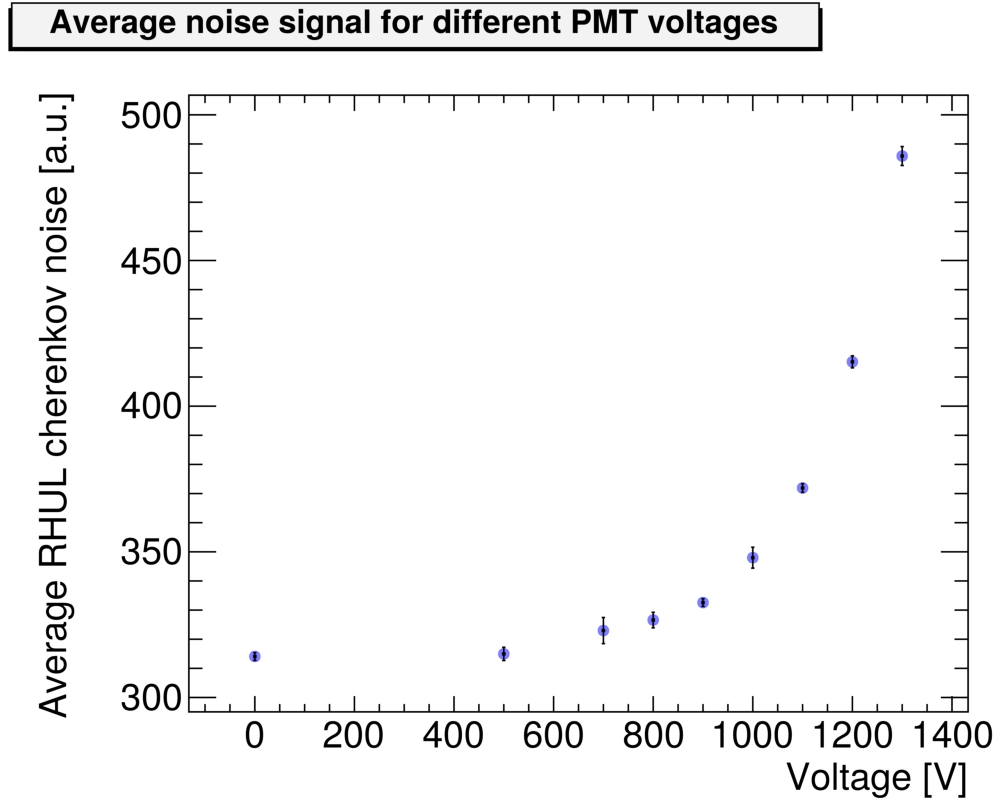
\includegraphics[width=0.99\textwidth]{Figures/ATF/AverageNoise_perVoltage_08April.pdf}
\caption{RHUL Cherenkov detector noise}
\end{subfigure}
\hfill
\begin{subfigure}[b]{0.49\textwidth}
  \centering
  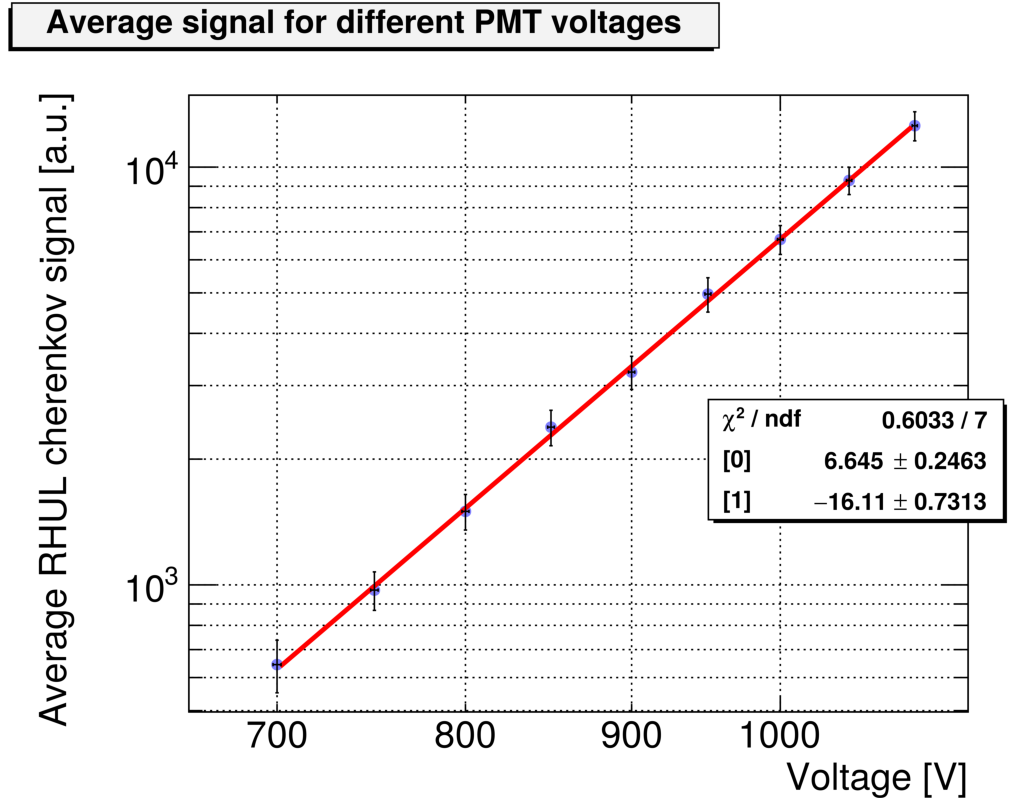
\includegraphics[width=\textwidth]{Figures/ATF/VoltageNormalization_totError.pdf}
\caption{RHUL Cherenkov detector voltage calibration}
\end{subfigure}
\caption[RHUL Cherenkov detector calibrations]{
Calibration measurements with the RHUL Cherenkov detector.
\\Figure (a) shows the average PMT noise signal as a function of the voltage applied to the detector PMT.
The noise was measured when the ATF beam was turned off. 
For each voltage, 500 or 1000 ADC pulses of noise were recorded, and the noise was averaged over the number of pulses. 
\\Figure (b) shows the average PMT signal as a function of the voltage applied to the detector PMT. 
The signal was measured when the ATF beam was stable at a beam intensity of \num[detect-all]{0.15}$\pm$\num[detect-all]{0.02e10}. 
For each voltage, 500 ADC pulses were recorded, and the signal was averaged over the number of pulses.}
\label{fig:AverageNoise_VoltageNormalization}
\end{figure}

\paragraph{PMT voltage calibration measurements}

In order to compare data sets that are taken at different PMT voltages, the signals have to be scaled. 
The rule of scaling the data is derived from the fit to the calibration measurements in Figure~\ref{fig:AverageNoise_VoltageNormalization} (b). 
The data for this calibration is taken for stable beam conditions at a beam intensity of \num{0.15}$\pm$\num{0.02e10}, and then plotted in a double logarithmic plot. 
The linearity of the data points shows the behavior of the PMT for different voltages according to Equation~\ref{eq:PMTgain}~\cite{Hamamatsu}:
\begin{equation}
 \mu = A \cdot V^{kn} 
 \label{eq:PMTgain}
\end{equation}
where $\mu$ is the PMT gain, $V$ the applied voltage, and $n$ the number of anodes in the PMT. 
$A$ and $k$ are free parameters. 
This equation can be rewritten as:
\begin{equation}
 signal = par_1 \cdot V^{par_2}
 \label{eq:PMTgain_simple}
\end{equation}
After taking the logarithmic of both sides, the equation can be written as:
\begin{alignat}{4}
 & log(signal) & = & log(par_1) & + & par_2 & \cdot &log(V) \label{eq:PMTgain_log} \\
 & y & = & \{1\} & + & \{0\} & \cdot & x \label{eq:fit_function}
\end{alignat}
Equation~\ref{eq:PMTgain_log} proves the linearity of the graph in the double logarithmic plot and verifies Equation~\ref{eq:PMTgain} from the literature. 
For the log-log plot, Equation~\ref{eq:fit_function} is the derived fit function with the fit parameters that are obtained by applying the fit to the data in Figure~\ref{fig:AverageNoise_VoltageNormalization} (b). 
The original signal function is therefore:
\begin{equation}
 signal = 10^{\{1\}} \cdot V^{\{0\}}
 \label{eq:PMTgain_simple_fitparameters}
\end{equation}
with $log(par_1)$ being the fit parameter $\{1\}$, and $par_2$ being the fit parameter $\{0\}$.\\
A signal ($signal_1$) can then be scaled into a new signal ($signal_2$) according to the voltages by doing:
\begin{align}
 \frac{signal_1}{signal_2} & = \frac{10^{\{1\}}\cdot V_1^{\{0\}}}{10^{\{1\}}\cdot V_2^{\{0\}}} \\
 signal_2 & = signal_1 \cdot \left( \frac{V_2}{V_1} \right) ^{\{0\}}
\end{align}


\subsubsection{Collimator apertures scan at different intensities and vacuum pressures}
\label{aperture_scans}
For the measurements of the background signal in dependency of the collimator aperture, scans of the collimator apertures were done, whilst closing the collimator jaws simultaneously. 
Figure ~\ref{fig:AverageSignal_Aperture_Symmetric} (a) shows the plot of the average detector signals at five different beam intensities. 
It is clear that the background level rises with increasing intensity. 
The characteristic shape of the scan is however conserved: 
the background level is constant when closing the collimator from a full aperture of \SI{24}{\milli\metre} to about \SI{15}{\milli\metre}. 
When closing to \SI{10}{\milli\metre} the background level drops, and rises again when closing the collimator completely, i.e. to \SI{6}{\milli\metre} full aperture. 
\\The measurements shown in Figure~\ref{fig:AverageSignal_Aperture_Symmetric} (b) were done in a similar way but for two different vacuum pressures: \SI{4.9e-7}{\pascal} and \SI{1.06e-6}{\pascal}. 
The data were taken for a beam intensity of \num{0.5}$\pm$\num{0.03e10}. 
The background level is higher for a higher vacuum pressure, as expected. 
Nevertheless, the background level is not only shifted. 
At the plateau (between 12 and \SI{24}{\milli\metre}), the background level for the higher pressure is larger by almost a factor of two.
At an aperture of \SI{10}{\milli\metre}, however, the background is reduced to almost the same level at both pressures. 
The collimator therefore reduces the background dramatically, especially at high background rates.

\begin{figure}
\centering
\begin{subfigure}[b]{0.49\textwidth}
 \centering
 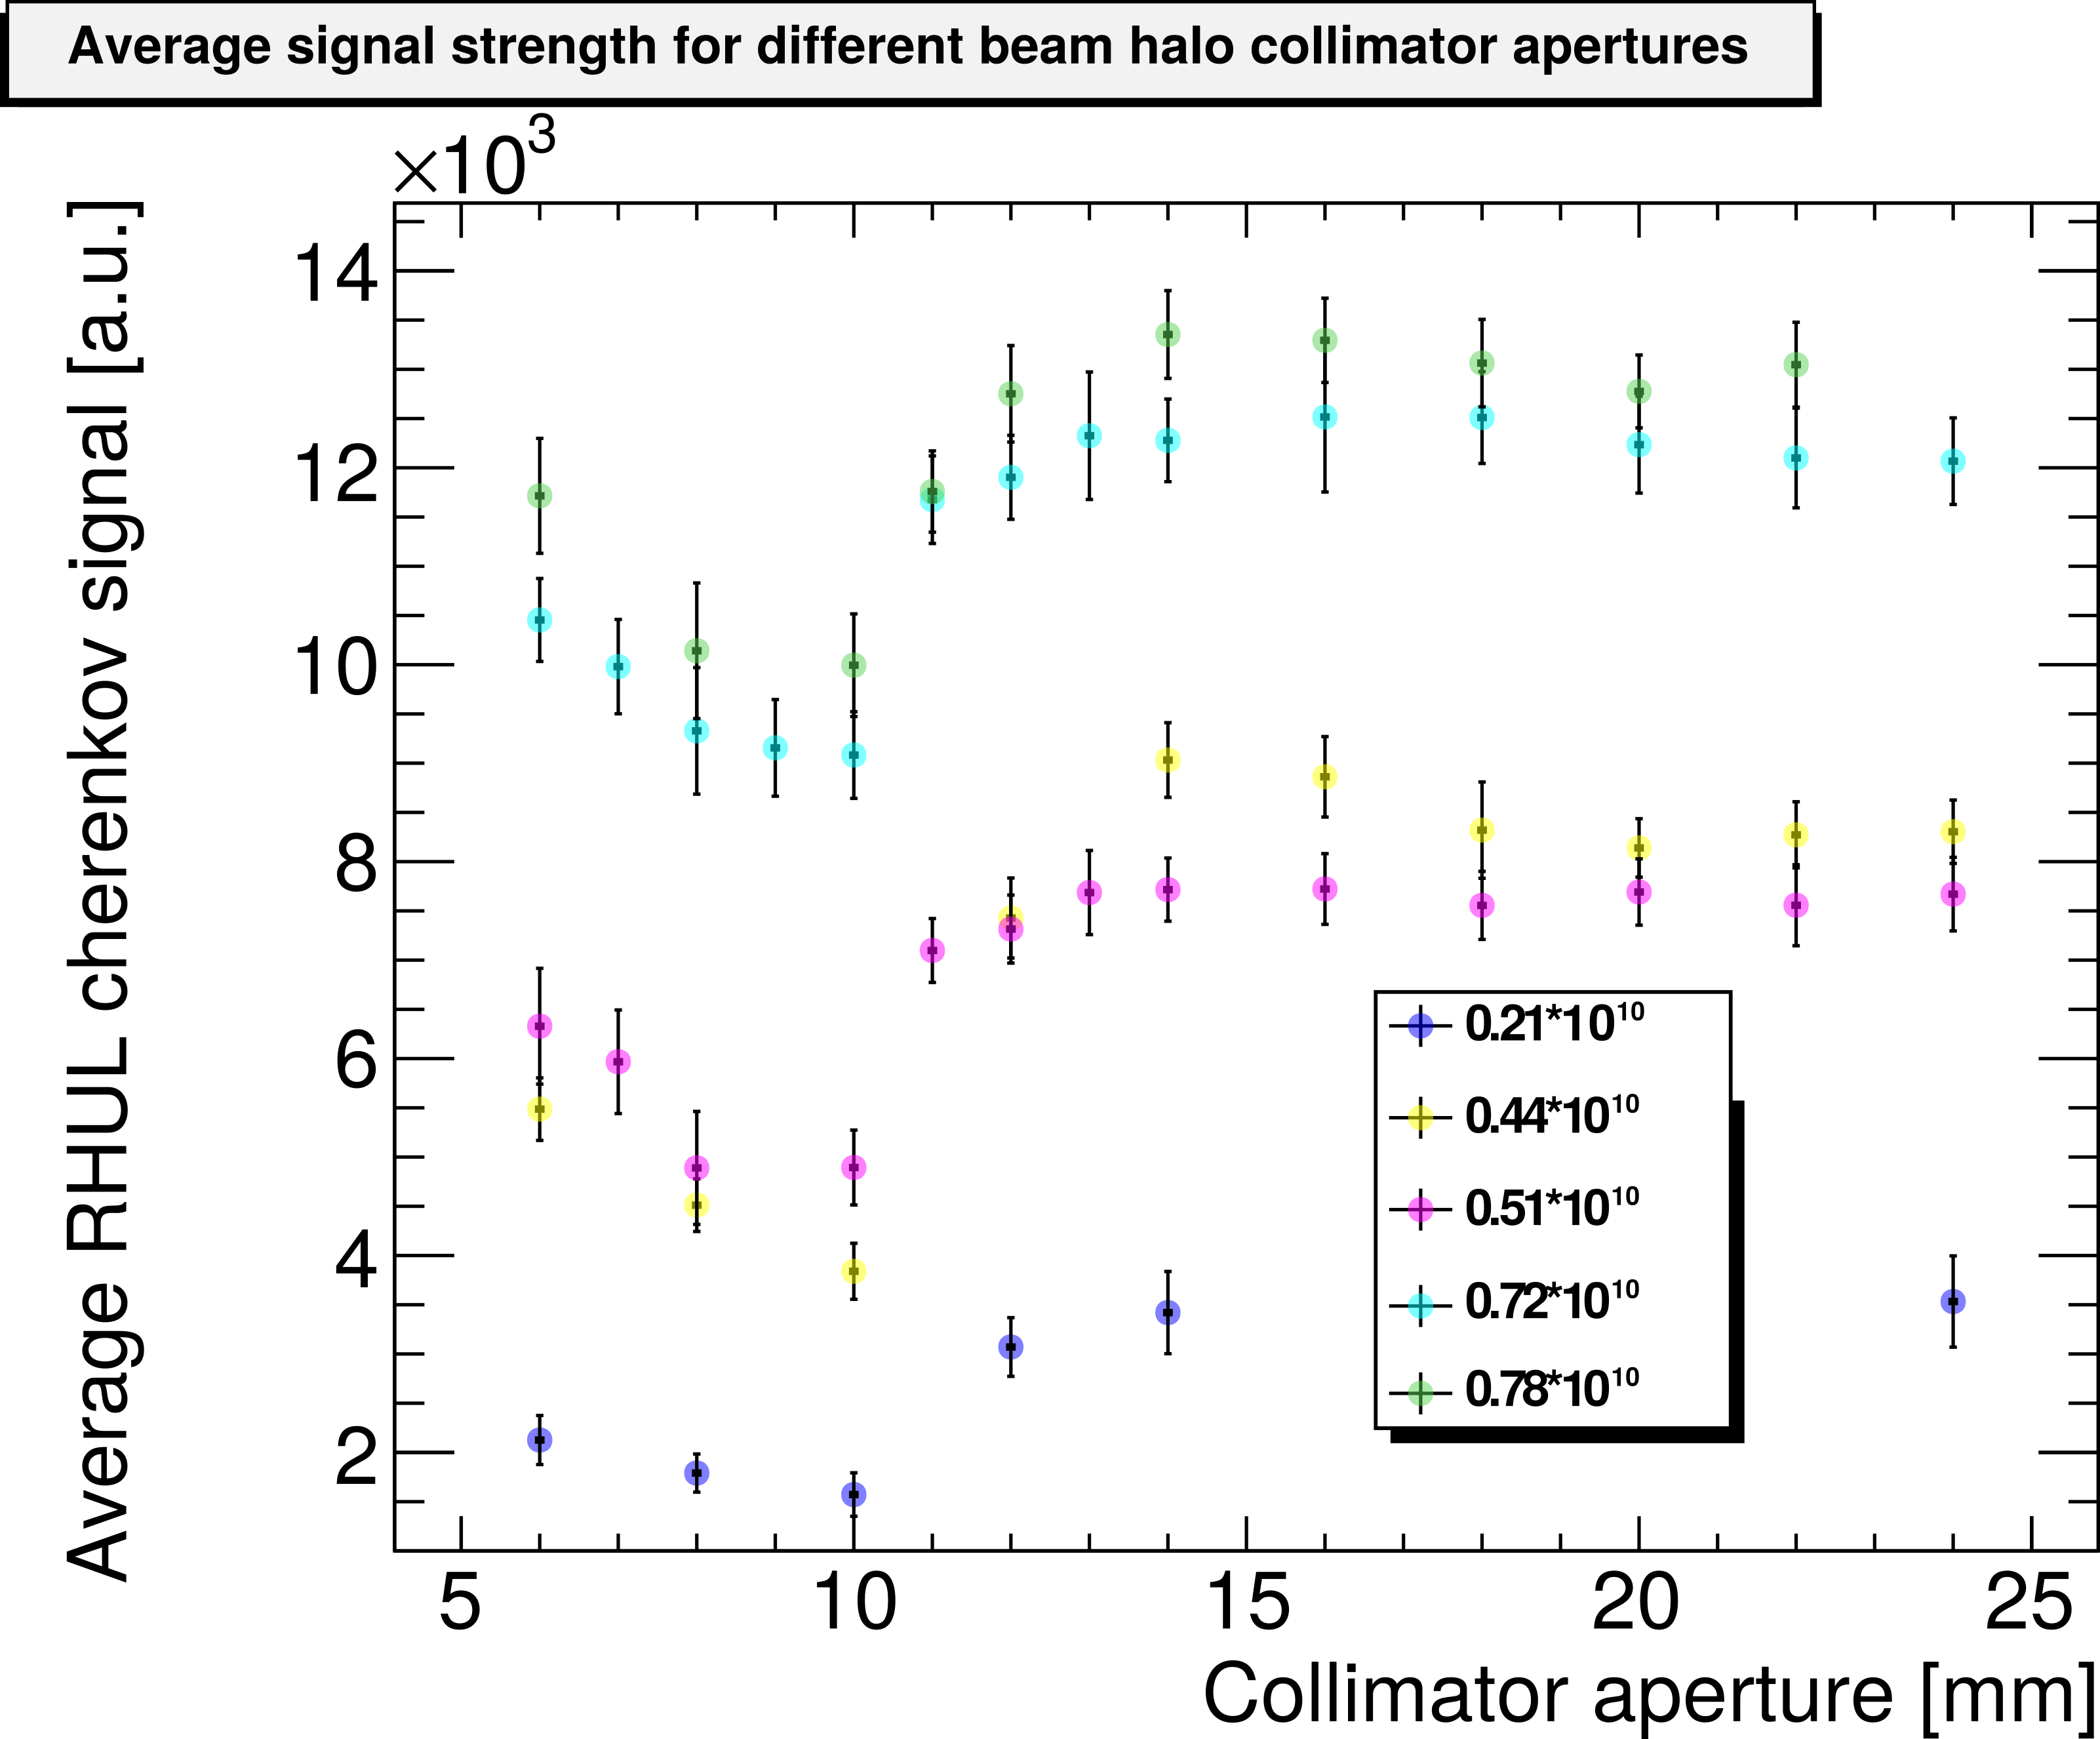
\includegraphics[width=\textwidth]{Figures/ATF/AverageSignal_perAperture.png}
 \caption{Different beam intensities}
\end{subfigure}
\hfill
\begin{subfigure}[b]{0.49\textwidth}
  \centering
 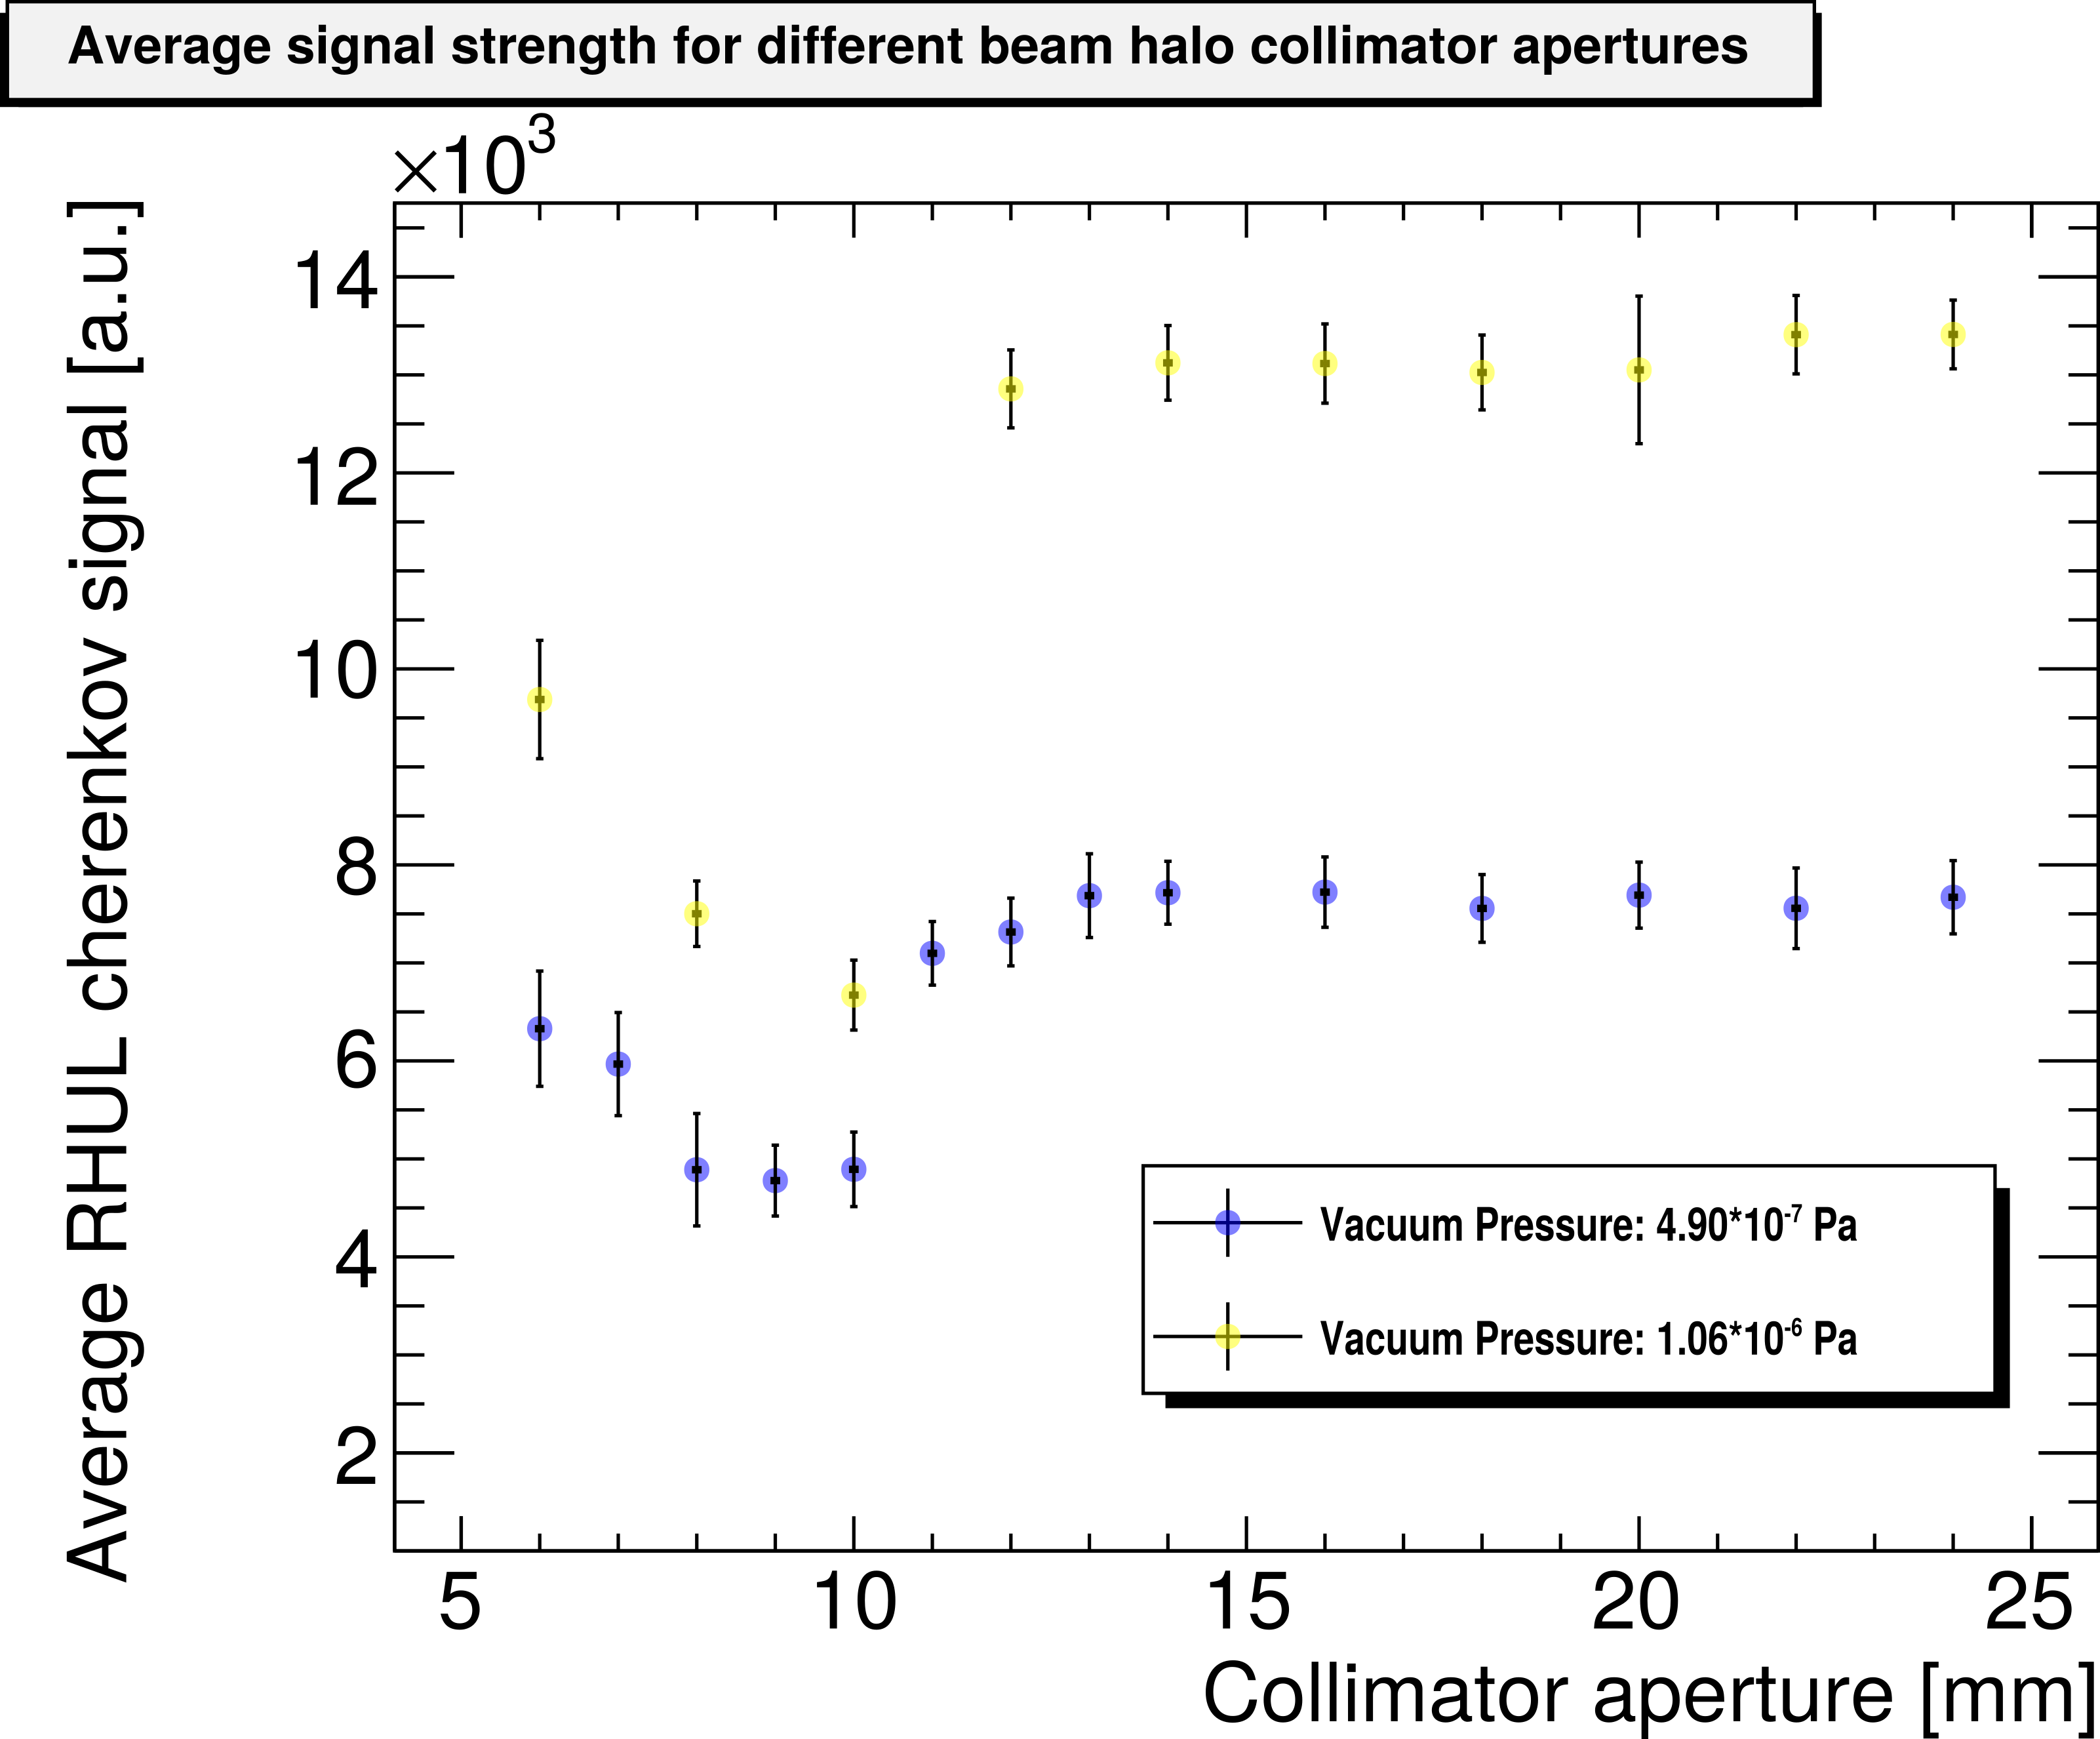
\includegraphics[width=\textwidth]{Figures/ATF/AverageSignal_perAperture_VacuumPressures.png}
 \caption{Different vacuum pressures}
\end{subfigure}
\caption[RHUL Cherenkov detector signal vs. collimator aperture]{
Average signal as a function of the full aperture of the vertical beam halo collimator. 
For Figure (a), the signal was measured for different beam intensities [\num[detect-all]{e10}]: 0.21$\pm$0.02, 0.44$\pm$0.02, 0.51$\pm$0.02, 0.72$\pm$0.02 and 0.78$\pm$0.02. 
\\For Figure (b), the signal was measured for a beam intensity of \num[detect-all]{0.5}$\pm$\num[detect-all]{0.03e10}. 
The vacuum pressure was lowered from \SI[detect-all]{4.9e-7}{\pascal} to \SI[detect-all]{1.06e-6}{\pascal}. 
\\For each aperture, 500 ADC pulses were recorded, and the signal was averaged over the number of pulses.}
\label{fig:AverageSignal_Aperture_Symmetric}
\end{figure}

The drop in the measurable background level for a collimator aperture between 15 and \SI{10}{\milli\metre} is on the one hand proof of principle for the collimator.
On the other hand, the measured rise in the background level leaves some questions open about the origin of the background particles and the effect of the collimator aperture on particle showers.
\\These questions are addressed in Section~\ref{sec:BDSIM_sim}, in which the effect of the collimator is simulated with \bdsim.

%---------------------------------------------------
\subsection{Simulation study of the vertical beam halo collimator}
\label{sec:BDSIM_sim}
As the data in Figure~\ref{fig:AverageSignal_Aperture_Symmetric} in the previous section have shown, the collimator reduces the existing background level if closed to a full aperture of \SI{10}{\milli\metre}. 
By closing the jaws further, the background level increases again.
To address open questions, simulations of the ATF2 lattice including the beam halo collimator were done using \bdsim.
The geometry model of the ATF2 accelerator lattice (in its state in the year 2015) already exists as a feature of \bdsim.
However, a realistic model of the vertical beam halo collimator had to be added.

\subsubsection{\bdsim}
\label{BDSIM}
\bdsim~\cite{BDSIM} is a \geant extension toolkit for the simulation of particle transport in accelerator beam lines, but also for the simulation of the interaction between the beam particles and the accelerator material. 
It is developed and supported by RHUL.
The geometry of lattice parts are described in classes within the \bdsim framework. 
Particle accelerator lattices, such as the ATF2 lattice, can easily be built up with the pre-defined components. 
The magnets and other beam line components available within \bdsim are simplified versions of common components used in particle accelerators. 
The ATF2 lattice is visualized with the \bdsim software in Figure~\ref{fig:ATF2_BDSIM}.
\\The simulation studies of ATF2, which are presented in this section were done with \bdsim version 0.95.
\begin{figure}[!h]
\centering
\includegraphics[width=0.7\textwidth]{Figures/ATF/atf_bdsim.png}
\caption[ATF2 lattice in \bdsim]{A part of the ATF2 lattice visualized with the \geant toolkit \bdsim.}
\label{fig:ATF2_BDSIM}
\end{figure}

\subsubsection{Modeling the vertical beam halo collimator}
The vertical beam halo collimator was modeled in GDML~\cite{GDML,GDML_web} format according to its technical design drawings.
Figure~\ref{fig:Collimator_model} shows a visualization of this model, as well as a view of the collimator structure inside the ATF2 lattice.
In Figure~\ref{fig:Collimator_model} (a), the collimator jaws can be seen, which can be set to an arbitrary y-position inside the structure.
With this new feature, \bdsim simulations with different collimator settings were done.
\begin{figure}[!h]
\centering
\begin{subfigure}[b]{0.49\textwidth}
 \centering
 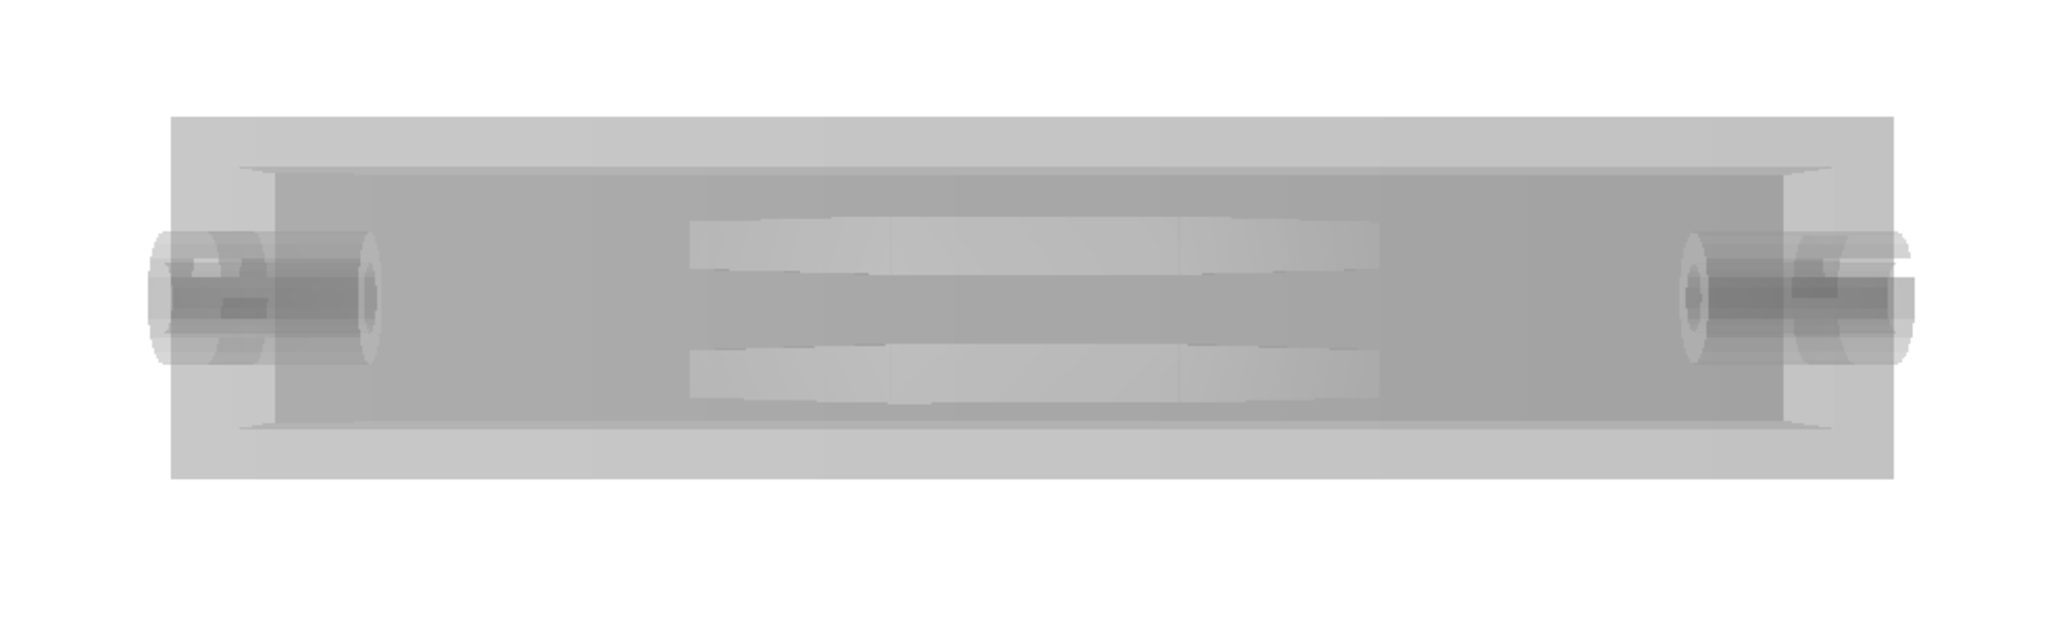
\includegraphics[width=\textwidth]{Figures/ATF/Collimator_model.pdf}
 \caption{Geometry visualization}
\end{subfigure}
\hfill
\begin{subfigure}[b]{0.49\textwidth}
  \centering
 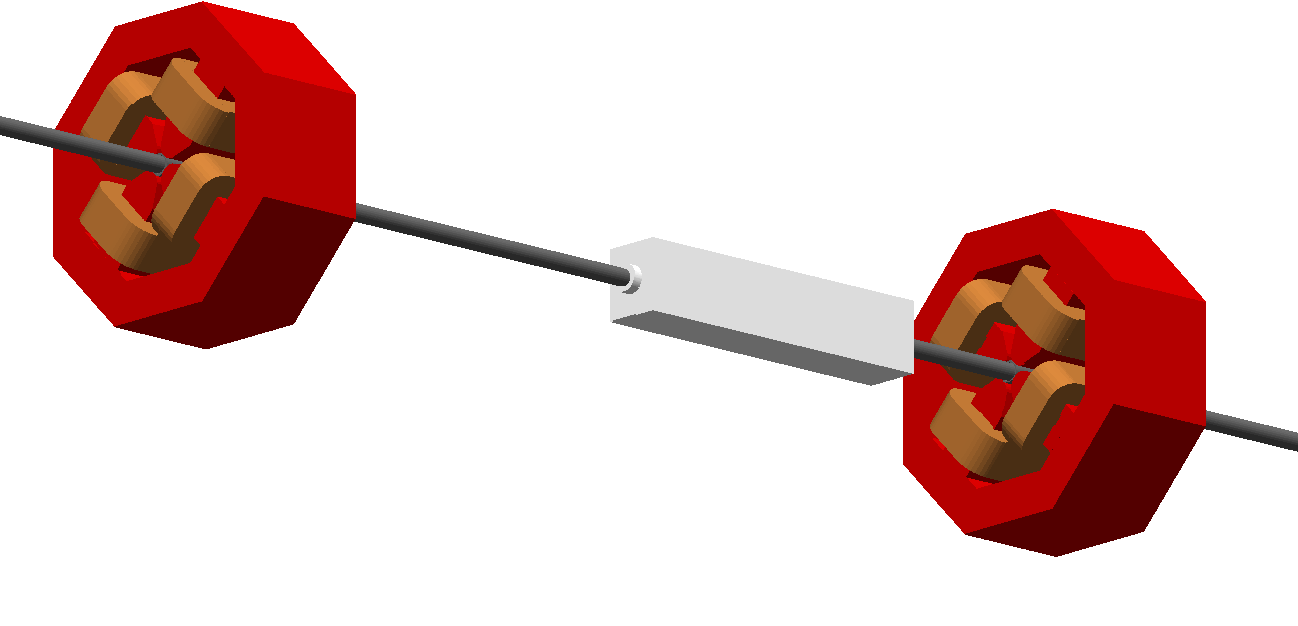
\includegraphics[width=0.9\textwidth]{Figures/ATF/Collimator_in_ATF2.png}
 \caption{Collimator model in the ATF2 beam line}
\end{subfigure}
\caption[Model of the vertical beam halo collimator used in the \bdsim simulation]{Model of the vertical beam halo collimator, used in the \bdsim simulation of the ATF2 beam line lattice.
}
\label{fig:Collimator_model}
\end{figure}

\subsubsection{Simulation results}
In order to validate the \bdsim simulation, comparisons of the beam parameter development along the beam line have been made for \bdsim and MADX~\cite{MADX}.
MADX is a simulation tool for the simulation of beam dynamics at particle accelerators.
For this validation, the beam size of the ATF2 beam core was plotted along the beam line for \bdsim and MADX.
As shown in Figure~\ref{fig:MADX}, both simulations of the ATF2 beam dynamics are in good agreement.
At the start of the ATF2 beam line, the beam core has a size of $\sigma^{Core}_x$ = \SI{51.9}{\micro\meter} and $\sigma^{Core}_y$ = \SI{15.4}{\micro\meter}.
At the location of the beam halo collimator ($S$ = \SI{9}{\meter}), the beam core has a size of $\sigma^{Core}_x$ = \SI{0.16}{\milli\meter} and $\sigma^{Core}_y$ = \SI{0.28}{\milli\meter}.
\begin{figure}[!h]
\centering
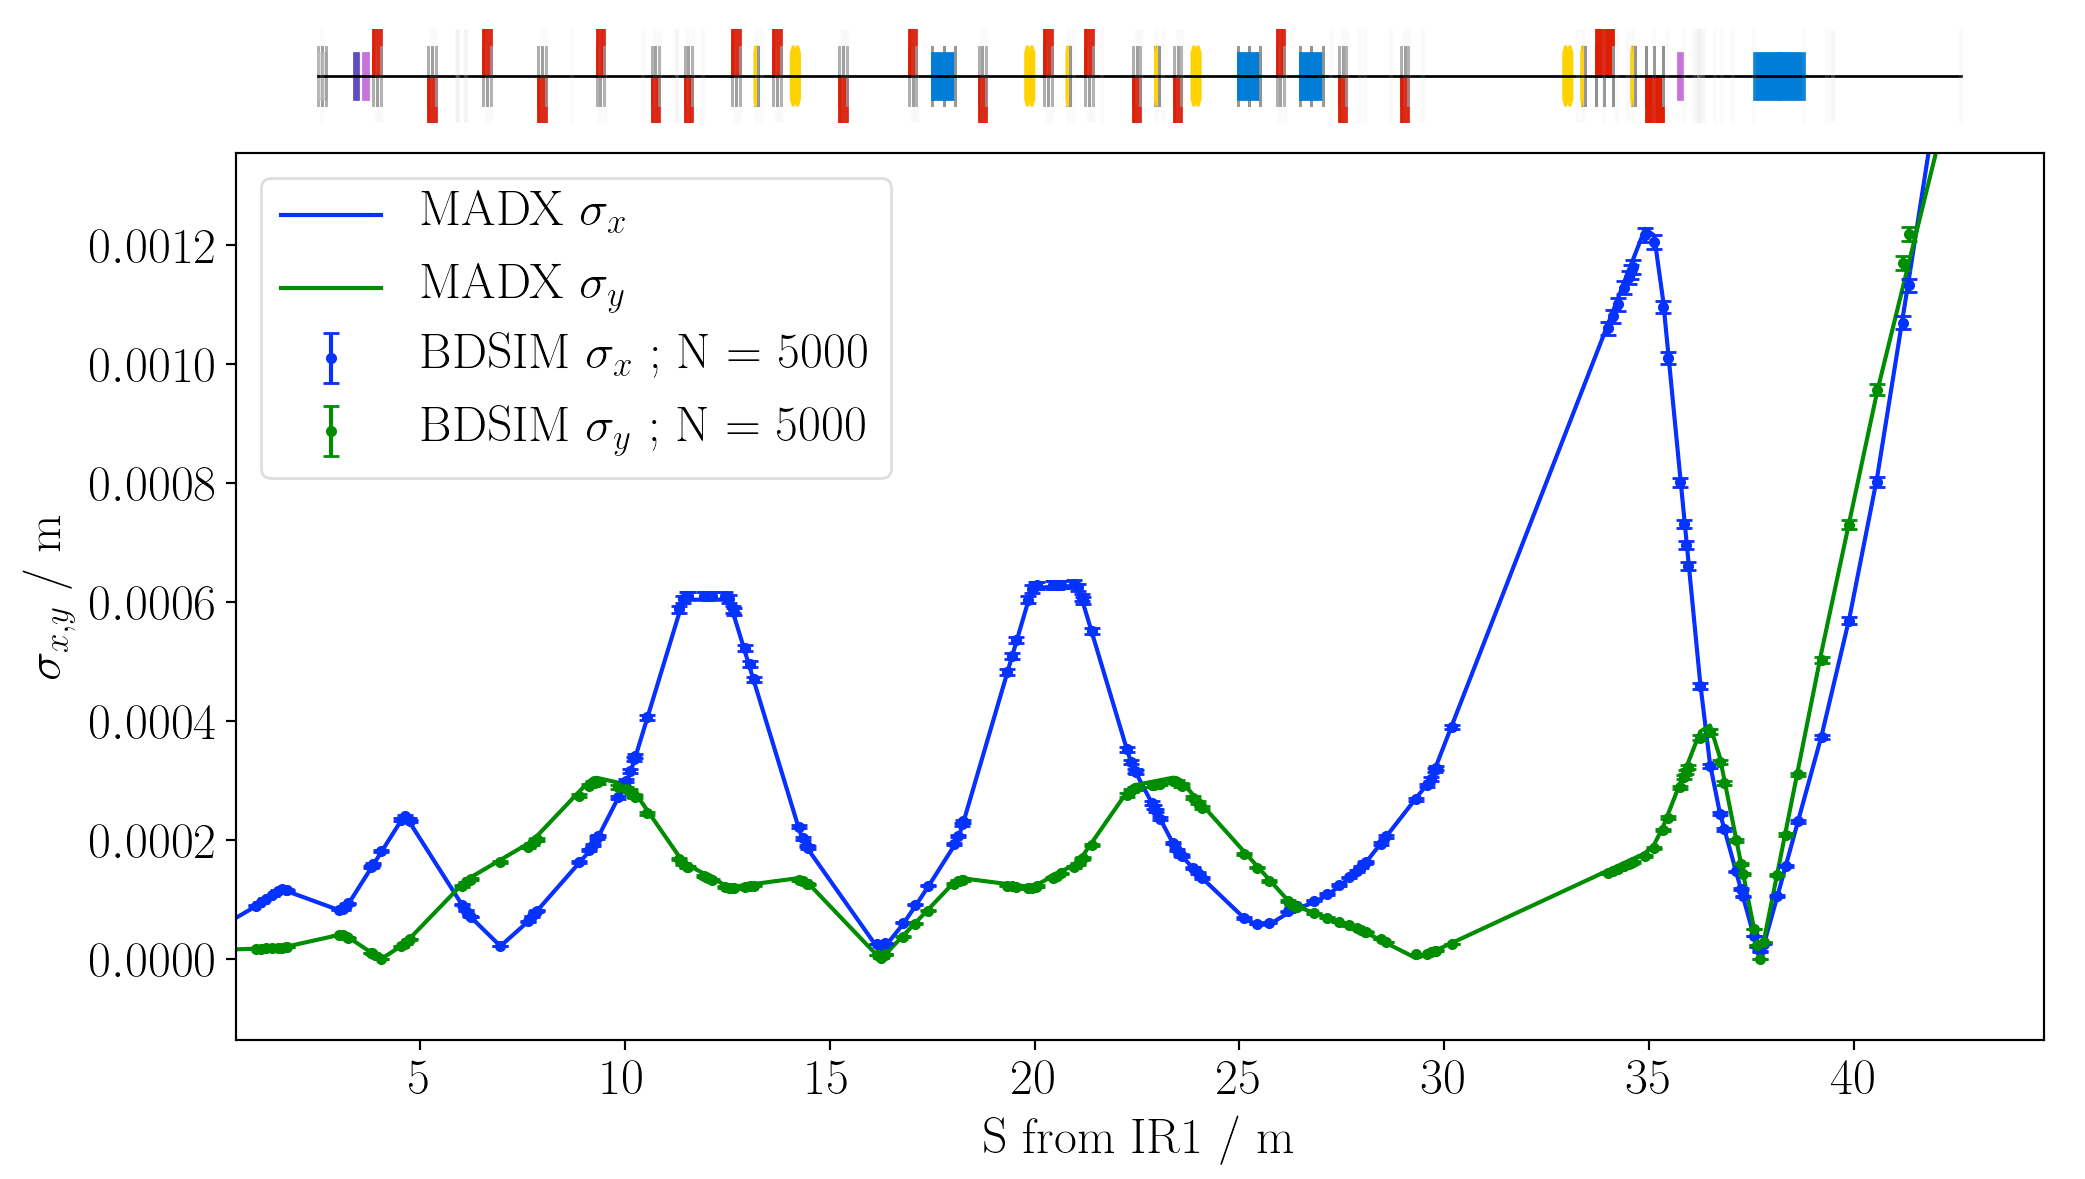
\includegraphics[width=0.7\textwidth]{Figures/ATF/pybdsim_sigma_gmadNuria.png}
\caption[Comparison of the ATF2 beam size development in \bdsim and MADX]{Comparison of the ATF2 beam size ($\sigma_x$ and $\sigma_y$) development along the beam line (S [m]) using \bdsim and MADX.}
\label{fig:MADX}
\end{figure}

For the \bdsim simulation of the background particles, the primary particle beam was then set to be the ATF2 beam halo, excluding the beam core.
The beam halo is defined to stretch from $3 \sigma^{Core}_x$ to $5 \sigma^{Core}_x$, and from $3 \sigma^{Core}_y$ to $10 \sigma^{Core}_y$.
In \bdsim, the beam halo is modeled accordingly, assuming a Gaussian distribution.
The beam particles have an energy of \SI{1.3}{\GeV} with an energy spread of \SI{0.08}{\percent}.
\\Several \bdsim simulation runs were done for different apertures of the vertical beam halo collimator.
The results were analyzed regarding the observable number of secondary particles created at the various ATF2 beam line components.
For a beam halo population of \num{2e6} primary particles, the number of secondary particles in the proximity of the beam halo collimator can be seen in Figure~\ref{fig:ParticlesPerModel}.
The number of particles are given in bar charts for the two collimator apertures: \SI{24}{\milli\meter} (open collimator) and \SI{4}{\milli\meter} (closed collimator).
In the direct proximity of the collimator, the number of secondary particles is larger in the case of a closed collimator due to particle showers caused by the intersection of the beam halo with the collimator jaws.
\\This is shown in Figure~\ref{fig:Particles_Collimator}.
The number of primary and secondary particles are plotted at the exit of the beam halo collimator for different collimator half apertures.
On the upper plots, the x- and y-positions of the primary beam particles are plotted.
For an open collimator, the beam is un-disrupted in both planes.
When closing the collimator, the cut-off of the beam halo is visible in the top right plot.
Primary particles are now, however, also spread in both the x- and y-direction.
The lower two plots show the positions of the secondary particles.
Again for an open collimator, the level of secondary shower particles is low.
For smaller collimator apertures, particle showers are created due to the intersection of the beam halo with the collimator jaws.
The background level rises by several orders of magnitude.
\\Figures~\ref{fig:ParticlesPerModel} (a) and (b) show furthermore that the number of secondaries further downstream of the collimator is smaller in every beam line component for a closed collimator compared to an open collimator, although more secondaries are produced in the direct proximity of the collimator.
The cut off beam halo, therefore, reduces the showers in downstream beam line components.
\\At the location of the RHUL Cherenkov detector, which is indicated in Figure~\ref{fig:ParticlesPerModel} (b), the number of occurring secondary particles is lower by over one order of magnitude in both cases compared to the components close to the collimator.
This indicates that the observation of differences in the background suppression by the vertical beam halo collimator is challenging at this location.

\begin{figure}
\centering
\begin{subfigure}[b]{0.49\textwidth}
 \centering
 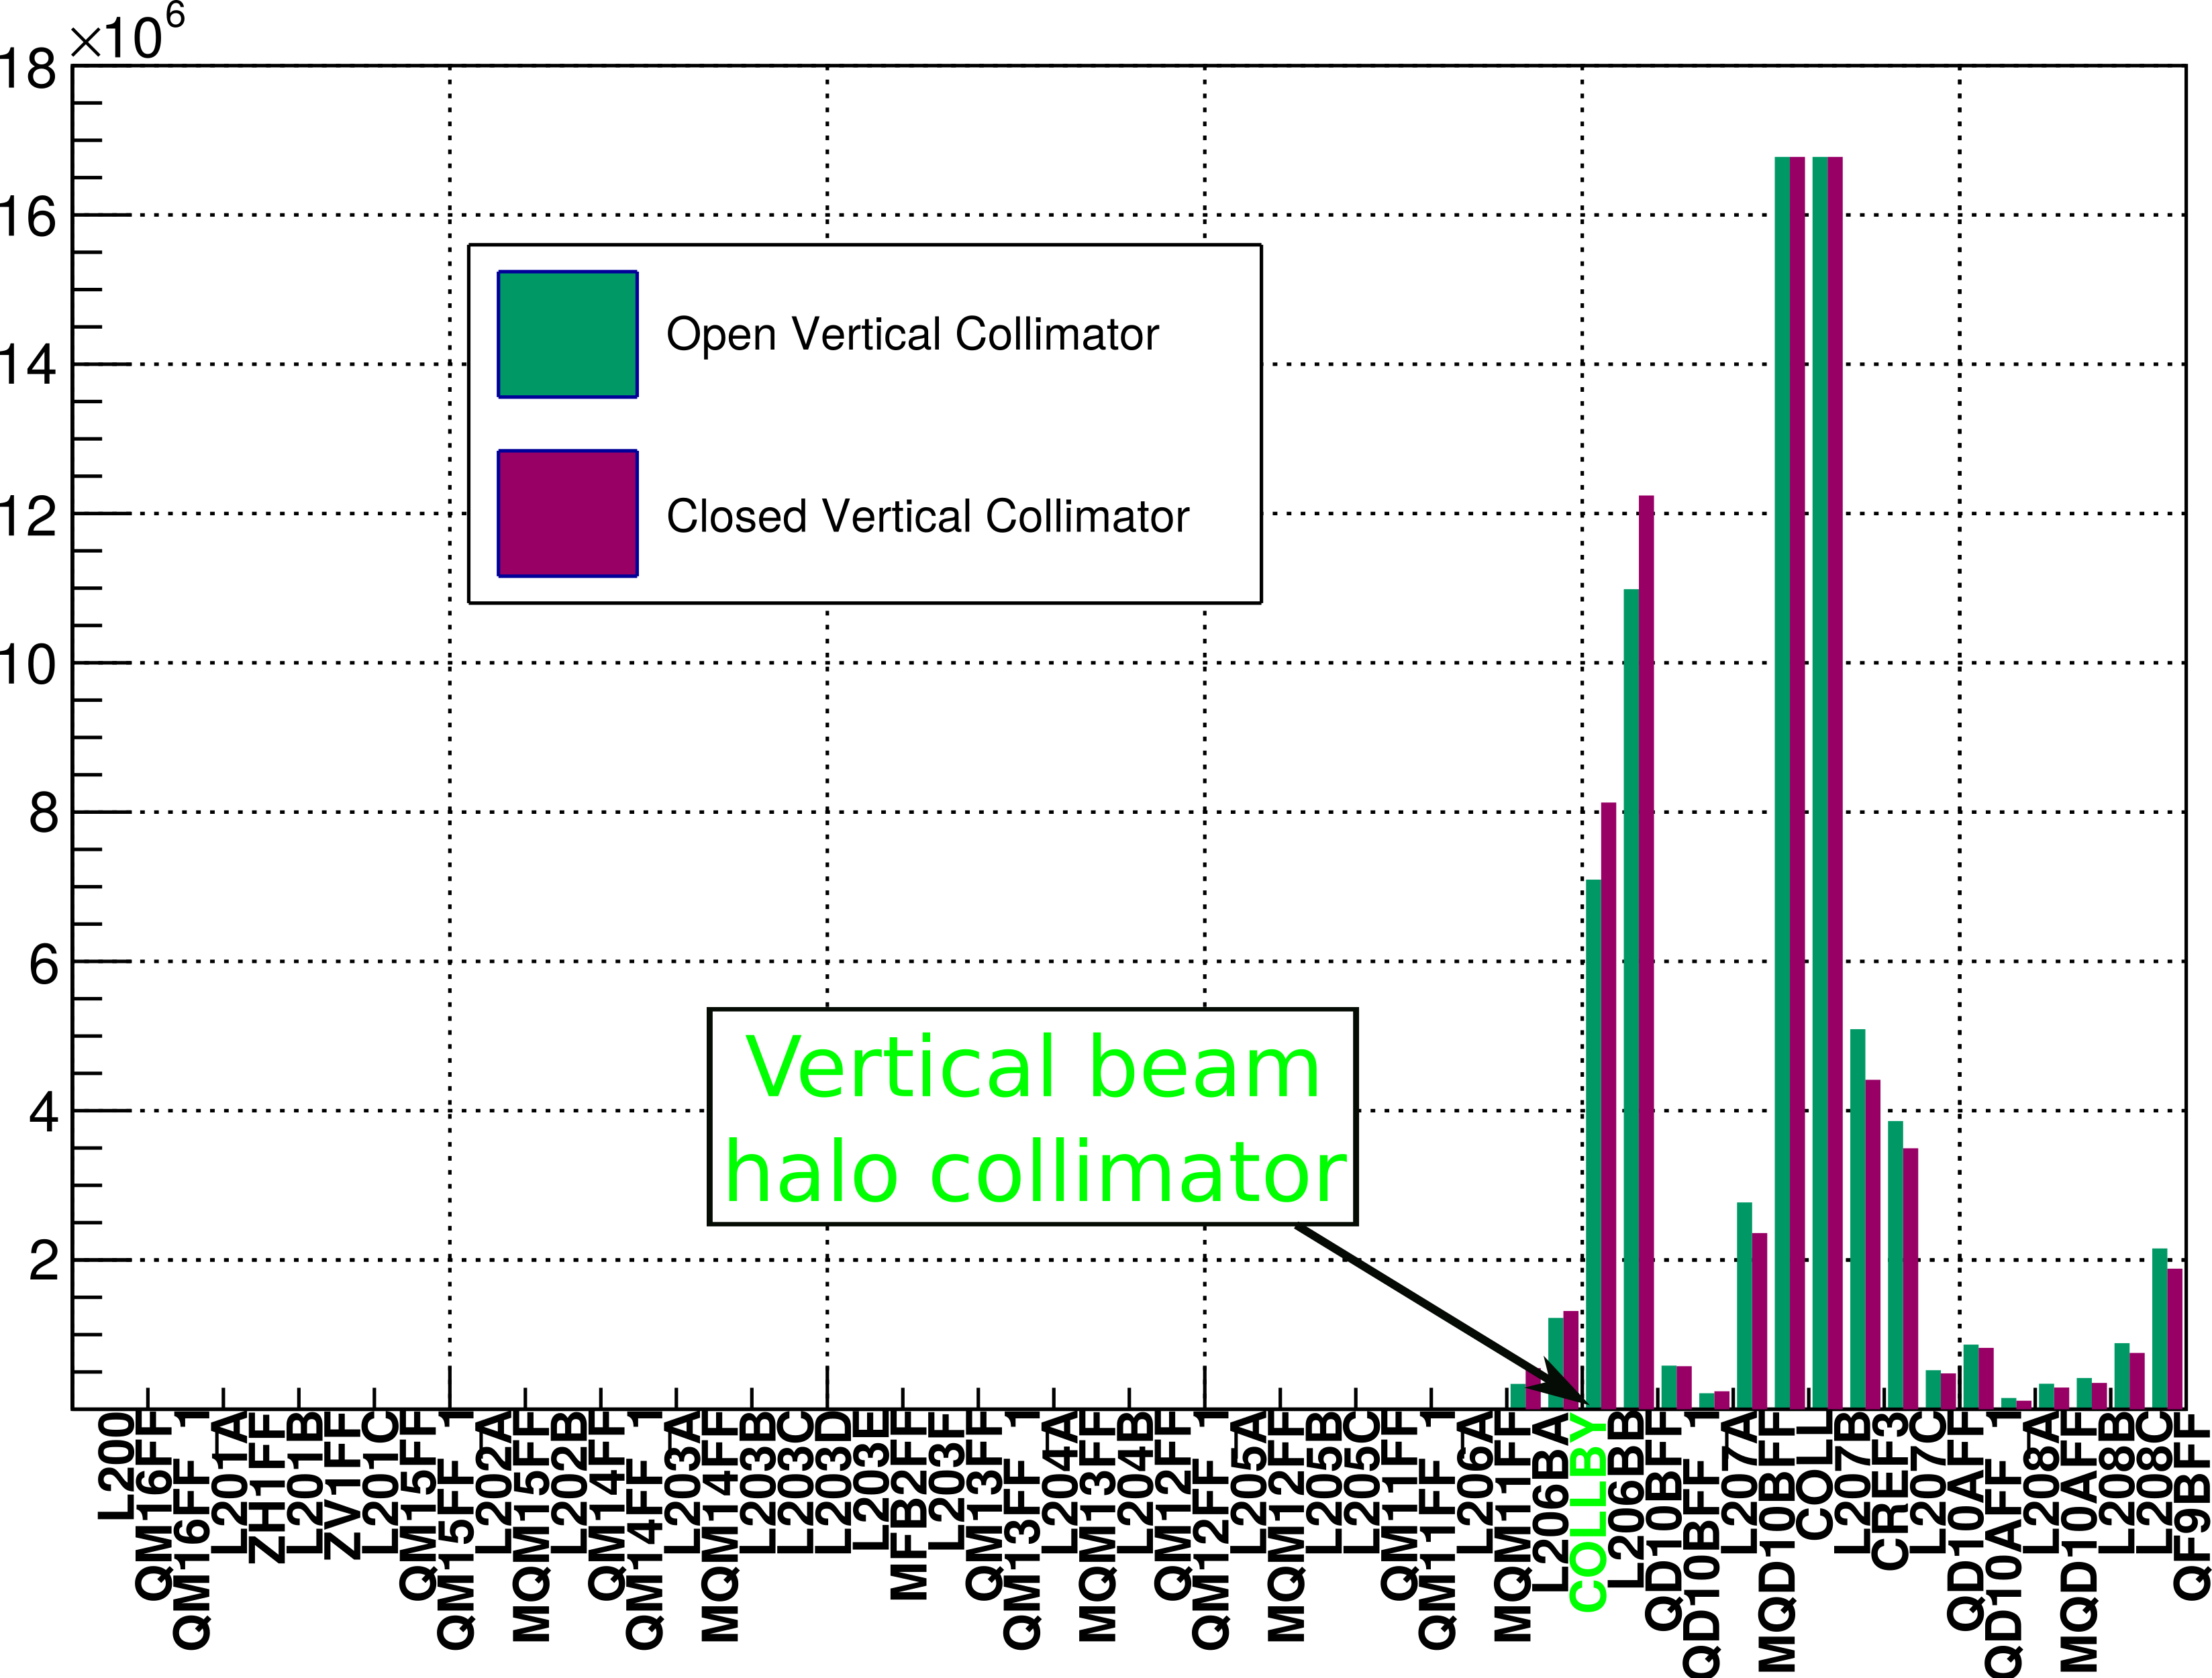
\includegraphics[width=\textwidth]{Figures/ATF/TracksPerModel_firstPart.png}
 \caption{Upstream ATF2 components}
\end{subfigure}
\hfill
\begin{subfigure}[b]{0.49\textwidth}
  \centering
 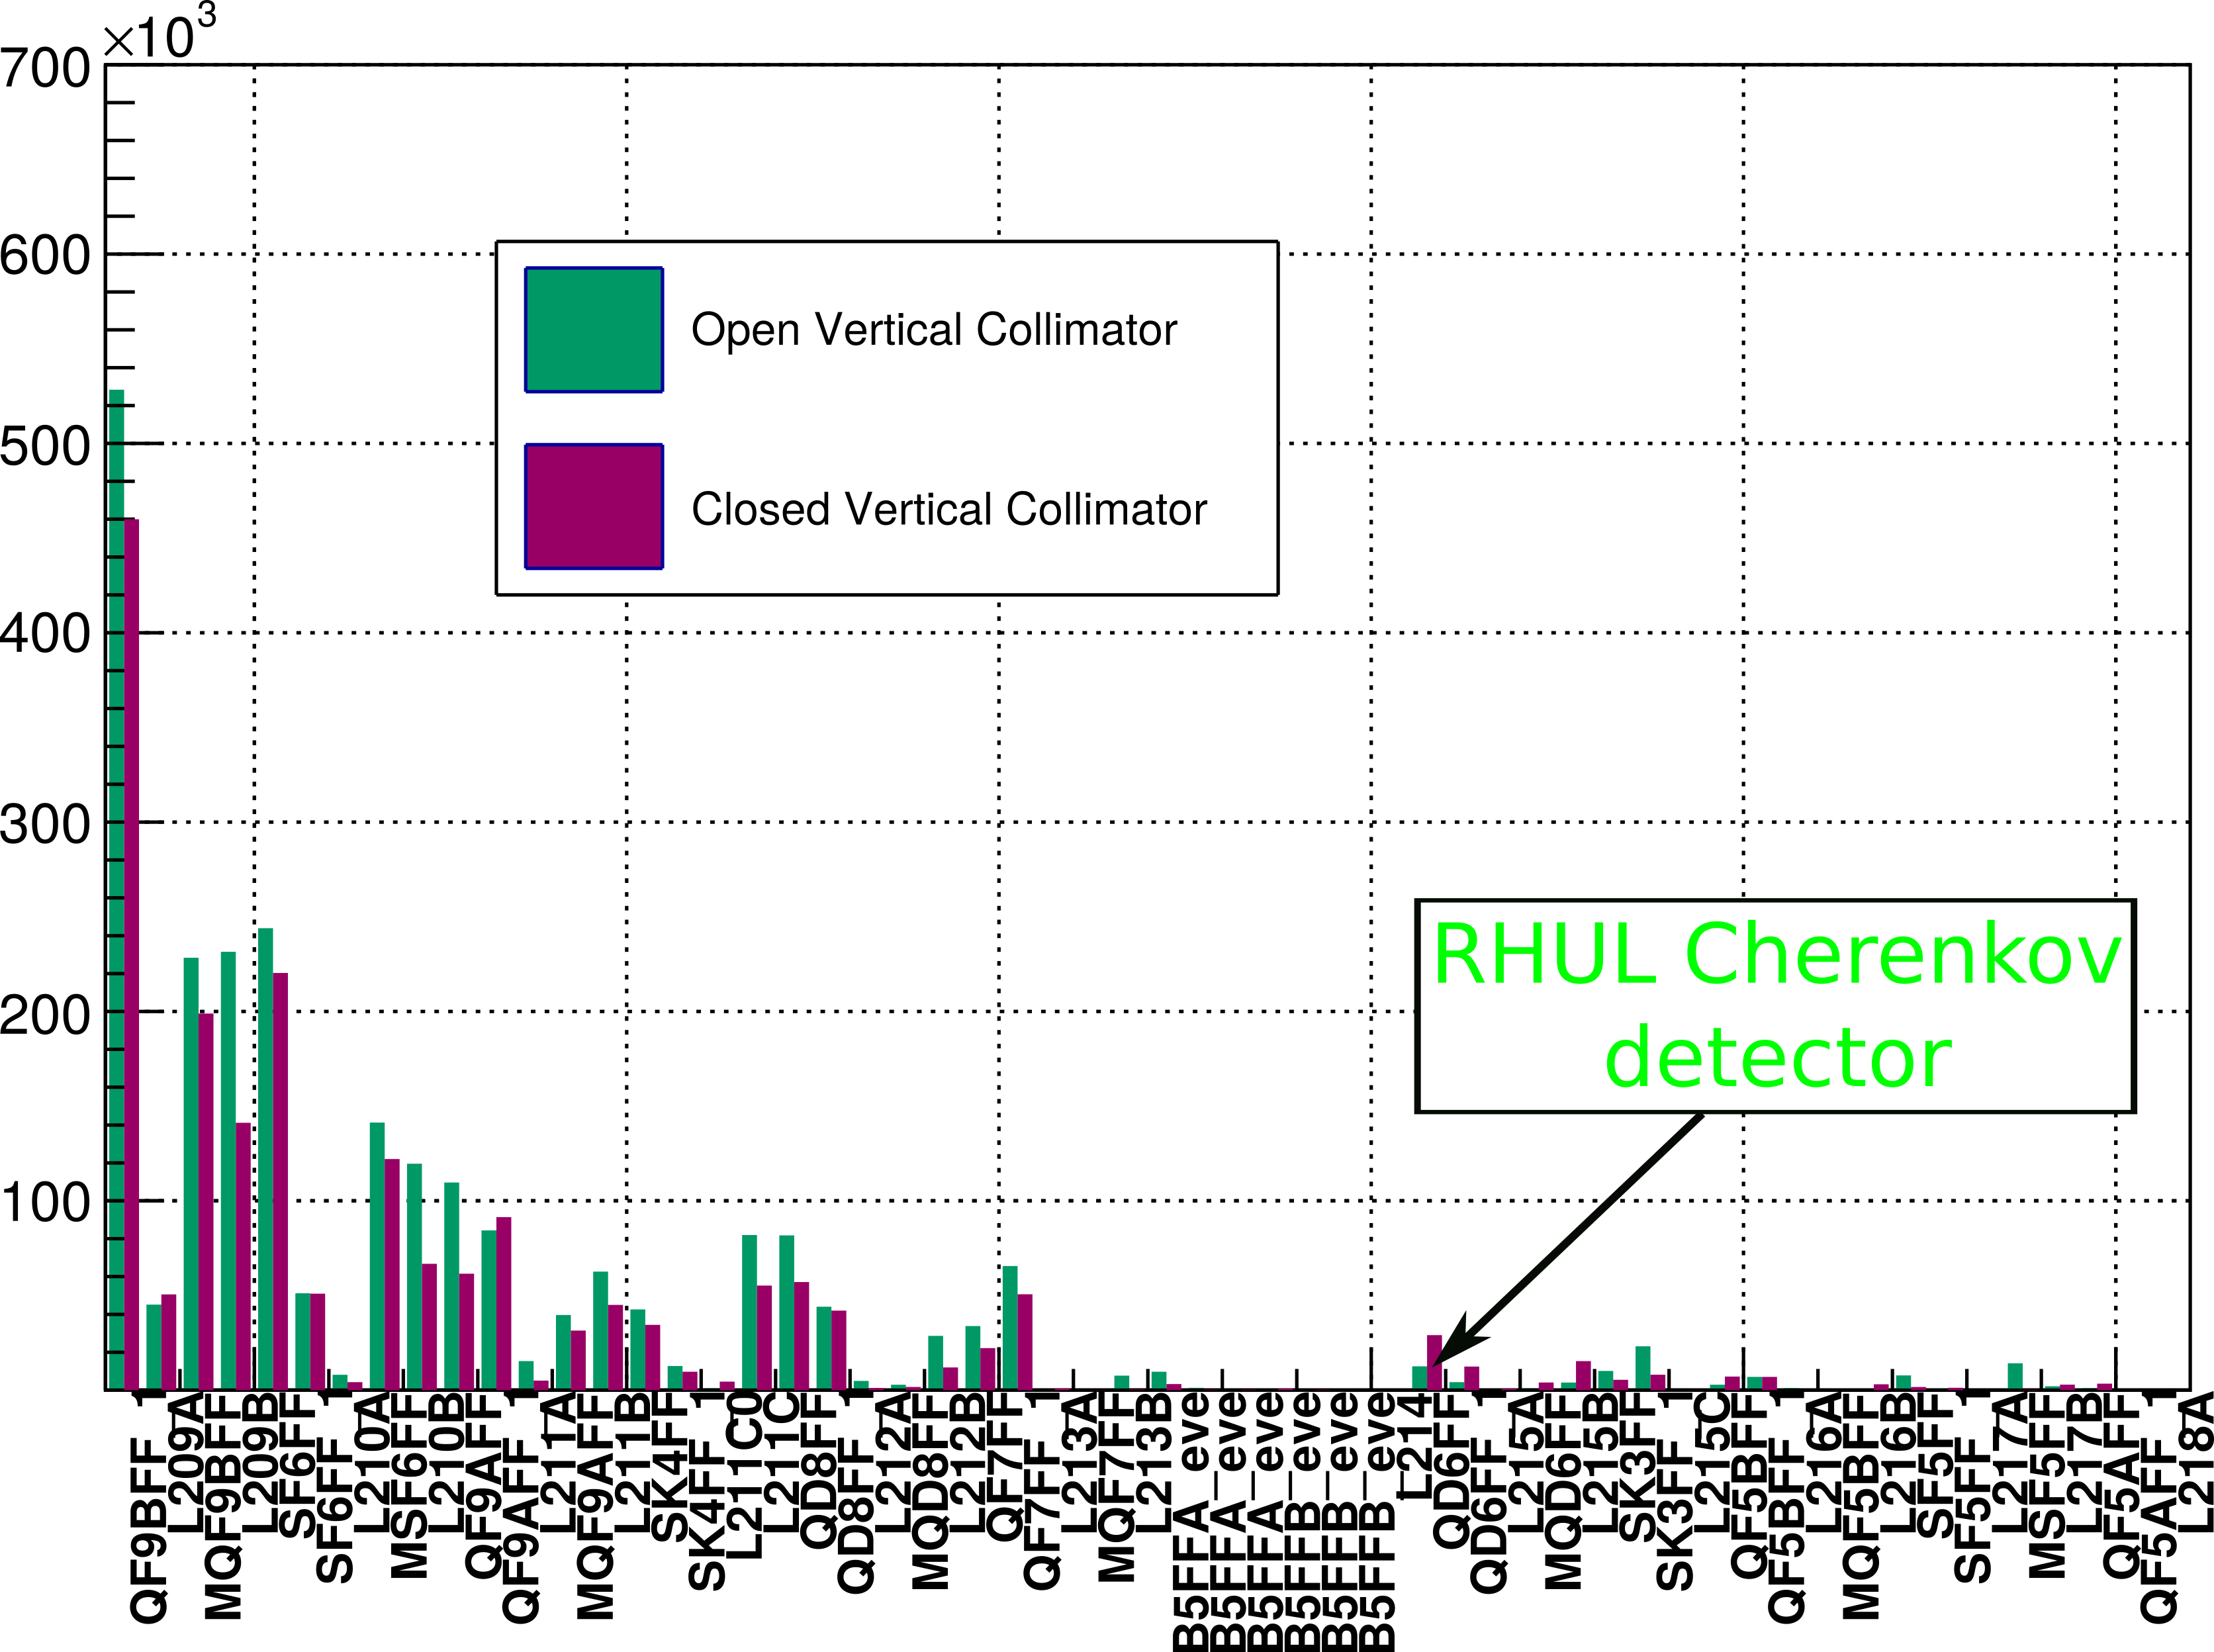
\includegraphics[width=\textwidth]{Figures/ATF/TracksPerModel_secondPart.png}
 \caption{Downstream ATF2 components}
\end{subfigure}
\caption[Number of secondary particles created in the ATF2 components]{Number of secondary particles observed in the ATF2 components directly upstream (a) and downstream (b) of the vertical beam halo collimator (COLLBY).
The x-axes show the component names in the ATF2 lattice.
Components starting with the letter ``L'' are drift lengths, components containing the word ``COLL'' are collimators.
All other names belong to magnet components.
\\The results for the ``Open Vertical Collimator'' are gained with fully retracted collimator jaws.
The ``Closed Vertical Collimator'' has a full aperture of \SI[detect-all]{4}{\milli\meter}.
}
\label{fig:ParticlesPerModel}
\end{figure}

\begin{figure}[!h]
\centering
\includegraphics[width=\textwidth]{Figures/ATF/Collimator_secondaries_Nuria_Thesis.png}
\caption[Number of particles at the beam halo collimator]{Number of primary and secondary particles arriving at the exit of the vertical beam halo collimator~\cite[cf. p. 152]{Nuria_Thesis}.
The upper plots show the number of primary particles in the x- and y-direction for different collimator half apertures.
A half aperture of \SI[detect-all]{12}{\milli\meter} corresponds to a completely open collimator (with a full aperture of \SI[detect-all]{24}{\milli\meter}).
\\The lower plots show the number of secondary particles in the x- and y-direction for the same collimator apertures.}
\label{fig:Particles_Collimator}
\end{figure}

Further studies have been conducted to find the origin of the particles that would hit the RHUL Cherenkov detector.
To this end, cuts have been applied to the particle positions, such that only particles with x- and y-positions within a window that matches the front face of the RHUL Cherenkov detector are registered.
The result is shown in Figure~\ref{fig:RHUL_Cherenkov_Sampler}.
The largest contribution are the primary beam particles.
Almost all other contributions are several orders of magnitude smaller.
The respective components are all located downstream of the beam halo collimator and upstream of the Cherenkov detector.
The number of observed shower particles coming directly from the beam halo collimator (COLLBY) is smaller for the closed collimator than for the open collimator by a few percent.
Overall, there is no significant difference in the number of particles between the two studied collimator apertures.

\begin{figure}[!h]
\centering
\includegraphics[width=0.6\textwidth]{Figures/ATF/RHUL_Cherenkov_Sampler1.png}
\caption[Number of particles at the RHUL Cherenkov detector]{Number of secondary particles arriving at the location of the RHUL Cherenkov detector in the case of an open (aperture of \SI[detect-all]{24}{\milli\meter}) and closed (aperture of \SI[detect-all]{4}{\milli\meter}) vertical beam halo collimator (COLLBY).
The x-axis shows the component names in the ATF2 lattice.
Components starting with the letter ``L'' are drift lengths, components containing the word ``COLL'' are collimators.
All other names belong to magnet components.}
\label{fig:RHUL_Cherenkov_Sampler}
\end{figure}

\subsection{Conclusion on the studies concerning the background levels in the proximity of the vertical beam halo collimator}
The presented \bdsim simulation studies of the ATF2 lattice and the effect of the vertical beam halo collimator does not yield the desired results comparable to the measured data, which were discussed in Section~\ref{aperture_scans}.
Figure~\ref{fig:ParticlesPerModel} shows that the level of secondary particles at the location of the RHUL Cherenkov detector is low in comparison to the direct proximity of the vertical beam halo collimator.
After discussions with \bdsim developers, it was concluded that the geometry models of the ATF2 beam line and its components are not mature enough for precision studies of the background in dependency of the collimator aperture.
In order to improve the model, more accurate measurements of all component apertures along the ATF2 line had to be taken and implemented.
The exact apertures are needed for a realistic simulation of the interaction of the beam halo with the beam line material.
Additionally, the magnetic fields around the beam line magnets, which also affect the secondary particles, have to be modeled outside the beam line.
So far, the implemented field maps only describe the magnetic field around the beam axis.
\\Overall, the analysis tool, which was written to gain the presented simulation results, is capable of showing the origin of the background particles and the background level at all components along the beam line.
The beam halo collimator model, which was created for this simulation study, was provided to the \bdsim developers for its implementation into the ATF2 lattice, which is part of the available examples given in the \bdsim framework.
\\For future studies, the background levels should be measured at locations closer to the beam halo collimator, where higher background levels are expected.
The effect of the collimator aperture is therefore easier to observe due to higher statistics and fewer influencing components between the collimator and the background detector.
Together with an improved \bdsim model of ATF2, various background studies could be conducted regarding the impact of accelerator components and accelerator running schemes.

\subsection{Effect on the background level at IP}
\label{collimator_bkg_IP}
In Section~\ref{aperture_scans}, it was shown that the background level measured with the RHUL Cherenkov detector is affected by the movement of the collimator jaws.
However, the actual aim of the vertical beam halo collimator is to reduce the machine background at the IP.
Figure~\ref{fig:IP_background} shows measurements of background photons at the ATF2 IP in dependency of the vertical beam halo aperture.
For all measured beam intensities, the background photon level was reduced by closing the collimator to a half aperture smaller than \SI{6}{\milli\meter}, which corresponds to a full aperture of \SI{12}{\milli\meter}.
This and further results concerning studies of the beam halo collimator~\cite{Nuria_Thesis} are a proof of principle for the vertical beam halo collimator.
\begin{figure}[!h]
\centering
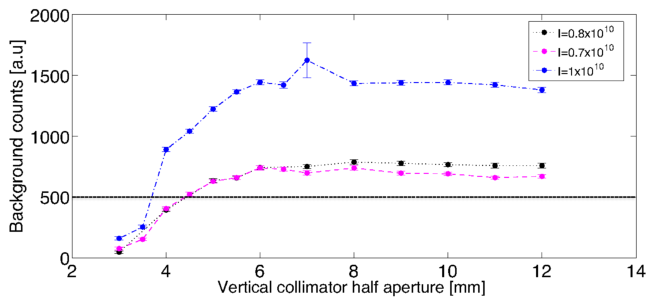
\includegraphics[width=0.7\textwidth]{Figures/ATF/IP_background_Nuria_Thesis_p212.pdf}
\caption[Number of background particles at the ATF2 IP]{Number of photons measured at the ATF2 IP in dependency of the vertical beam halo collimator aperture~\cite[p. 212]{Nuria_Thesis}.
The collimator aperture is given as the half aperture, which is the distance between the center axis and one collimator jaw.
The photons were measured behind the ATF2 IP, where the beam electrons are deflected by the last bending magnet of the beam line lattice.
\\The measurements were done for three beam intensities (\num[detect-all]{0.7e10}, \num[detect-all]{0.8e10}, and \num[detect-all]{1.0e10}).}
\label{fig:IP_background}
\end{figure}